%%%%%%%%%%%%%%%%%%%%%%% file template.tex %%%%%%%%%%%%%%%%%%%%%%%%%
%
% This is a general template file for the LaTeX package SVJour3
% for Springer journals.          Springer Heidelberg 2010/09/16
%
% Copy it to a new file with a new name and use it as the basis
% for your article. Delete % signs as needed.
%
% This template includes a few options for different layouts and
% content for various journals. Please consult a previous issue of
% your journal as needed.
%
%%%%%%%%%%%%%%%%%%%%%%%%%%%%%%%%%%%%%%%%%%%%%%%%%%%%%%%%%%%%%%%%%%%
%
% First comes an example EPS file -- just ignore it and
% proceed on the \documentclass line
% your LaTeX will extract the file if required
%\begin{filecontents*}{example.eps}
%!PS-Adobe-3.0 EPSF-3.0
%%BoundingBox: 19 19 221 221
%%CreationDate: Mon Sep 29 1997
%%Creator: programmed by hand (JK)
%%EndComments
%gsave
%newpath
%  20 20 moveto
%  20 220 lineto
%  220 220 lineto
%  220 20 lineto
%closepath
%2 setlinewidth
%gsave
%  .4 setgray fill
%grestore
%stroke
%grestore
%\end{filecontents*}
%
\RequirePackage{fix-cm}
%
%\documentclass{svjour3}                     % onecolumn (standard format)
%\documentclass[smallcondensed]{svjour3}     % onecolumn (ditto)
\documentclass[smallextended]{svjour3}       % onecolumn (second format)
%\documentclass[twocolumn]{svjour3}          % twocolumn
%
\smartqed  % flush right qed marks, e.g. at end of proof
%
% \usepackage{mathptmx}      % use Times fonts if available on your TeX system
%
% insert here the call for the packages your document requires
%\usepackage{latexsym}
% etc.
%
% please place your own definitions here and don't use \def but
% \newcommand{}{}
%
% Insert the name of "your journal" with
% \journalname{myjournal}
\usepackage[utf8]{inputenc}
\usepackage{graphicx, float}
\usepackage{amsmath, amssymb, amsfonts}
\usepackage{xcolor}
\definecolor{darkgreen}{rgb}{0.0, 0.5, 0.0}
\newcommand{\nisha}[1]{{\color{darkgreen} #1}}
\begin{document}

\title{On the probability of finding a nonphysical solution through shadowing}
\date{June 2020}
\subtitle{Do you have a subtitle?\\ If so, write it here}

%\titlerunning{Short form of title}        % if too long for running head

\author{Qiqi Wang}

%\authorrunning{Short form of author list} % if too long for running head

\institute{F. Author \at
              first address \\
              Tel.: +123-45-678910\\
              Fax: +123-45-678910\\
              \email{fauthor@example.com}           %  \\
%             \emph{Present address:} of F. Author  %  if needed
           \and
           S. Author \at
              second address
}

\date{Received: date / Accepted: date}
% The correct dates will be entered by the editor


\maketitle

\begin{abstract}
Insert your abstract here. Include keywords, PACS and mathematical
subject classification numbers as needed.
\keywords{First keyword \and Second keyword \and More}
% \PACS{PACS code1 \and PACS code2 \and more}
% \subclass{MSC code1 \and MSC code2 \and more}
\end{abstract}

\maketitle
\section{Shadowing and some applications}

Shadowing refers to the relationship between a pair of solutions to slightly different governing equations. The difference between the governing equations can be due to parameter perturbation or numerical error. The solution to one governing equation is said to shadow a solution to a second, slightly different equation if
the first solution stays close to the second solution for some amount of time.

The existence of arbitrarily long shadowing solutions for sufficiently similar governing equations
has been proven for invertible hyperbolic maps by Anosov \cite{anosov} and Bowen \cite{bowen}.
For non-hyperbolic systems, it is often possible to estimate the length of time for which shadowing
solutions exist \cite{grebogi}\cite{hammel}.

The existence of shadowing trajectories underlies many applications.
Numerical simulations of turbulent flows have been widely used to study its statistical behavior.
It is argued, based on shadowing, that such numerical simulations of chaotic dynamical systems can be
useful, despite the butterfly effect. Consider a numerical solution to a deterministic chaotic system with an initial condition $x$.
Because of numerical and modeling errors, there will typically be a small difference between the
true governing physics and the equations solved on a computer.  As the system is evolved forward
in time, this difference will be amplified exponentially due to the chaotic nature of the system.
The question therefore arises as to whether or not numerical solutions to chaotic systems, such
as turbulent flows, are related to the physics at all.  The existence of shadowing solutions
is used to argue for the usefulness of such numerical solutions.
When certain conditions for shadowing theorems are met, the numerical solution would be an
approximation to a ``true'' solution that satisfies the real governing physics.

Shadowing is also used in sensitivity analysis of chaotic dynamical systems.  In particular,
it is used in computing how long-time-averages in a chaotic system
respond to small perturbations in the governing equation. In this application, derivative
of the long-time-averages is computed using a solution to the perturbed governing equation
that shadows a solution to the unperturbed equation.  The Least Squares Shadowing \cite{qiqi-lss} method
uses this concept.

There is an implicit assumption in both of these applications.  The assumption is that
the shadowing trajectory is a ``physical'' trajectory, a trajectory on which
the long-time-average of a quantity is equal to the physical \nisha{can we remove the word ``physical'' before ensemble average?} ensemble average.
Not all solutions satisfying the physical governing equation are considered ``physical''
in this sense.  In high-Reynolds number fluid flows, for example, a steady-state, laminar flow solution may satisfy the Navier-Stokes equation. But such a solution would never be observed in reality because it is unstable, and any small perturbation
would trip it into turbulence. Unstable steady-state solutions are not the only
non-physical solution. Many chaotic dynamical systems have infinitely many periodic
solutions that are, similar to their steady counterpart, unstable. These trajectories can have a probability distribution that is remarkably different from that of a typically observed solution of the governing equation. It is also possible to effect significant change in the statistics of the true governing dynamics by introducing a minor parameter perturbation. Thus, although two trajectories, at slightly different parameters, may shadow each other, the long-time-averages of observables calculated using them, may not be close.    
As we will see
in the next section, even solutions that look ``chaotic'', i.e., unsteady and aperiodic, may not be physical. 

\section{What are physical and nonphysical solutions?}

Intuitively, we call a solution to a governing equation ``physical'' if
it represents what one would observe in a physical experiment.  In particular, the statistics measured from a physical solution match the statistics observed
in an experiment.   Not all solutions are physical.  A laminar flow
solution, despite satisfying the governing equation, does not produce the
turbulent statistics one would observe in a high-Reynolds number experiment. Such solutions are thus called nonphysical.

In this section, we first describe mathematically what distinguishes a physical
and a nonphysical solution.  We also explain theoretically why it is unlikely
to observe a nonphysical solution in an experiment.  We then give a few
examples of these almost-never-observed nonphysical solutions.

\subsection{Physical solutions}
What we typically call ``physical'' solutions to a governing equation satisfy the following
two criteria: \nisha{Is the term ``physical'' to mean the following common in fluid mechanics? If not, can we emphasize that we are defining it here? e.g. }
\begin{enumerate}
    \item Long-time-averaged, ``statistical'' quantities converges as time goes to infinity.
    Consider $u(t)$ as the solution to a chaotic governing equation, then for \nisha{a continuous/regular observable?}
    a smooth quantity of interest $J(u(t))$,
    \begin{equation} \label{longtimeavg}
        \lim_{T\to\infty}\frac1T \int_0^T J(u(t))\,dt
    \end{equation}
    exists.
    \item For almost any small perturbation to the initial condition $u(0)\to u'(0)$, the perturbed
    solution $u'(t)$ should have the same statistics, i.e.,
    \begin{equation}
        \lim_{T\to\infty}\frac1T \int_0^T J(u(t))\,dt
      = \lim_{T\to\infty}\frac1T \int_0^T J(u'(t))\,dt
    \end{equation}
\end{enumerate}

\begin{figure}[H] \centering
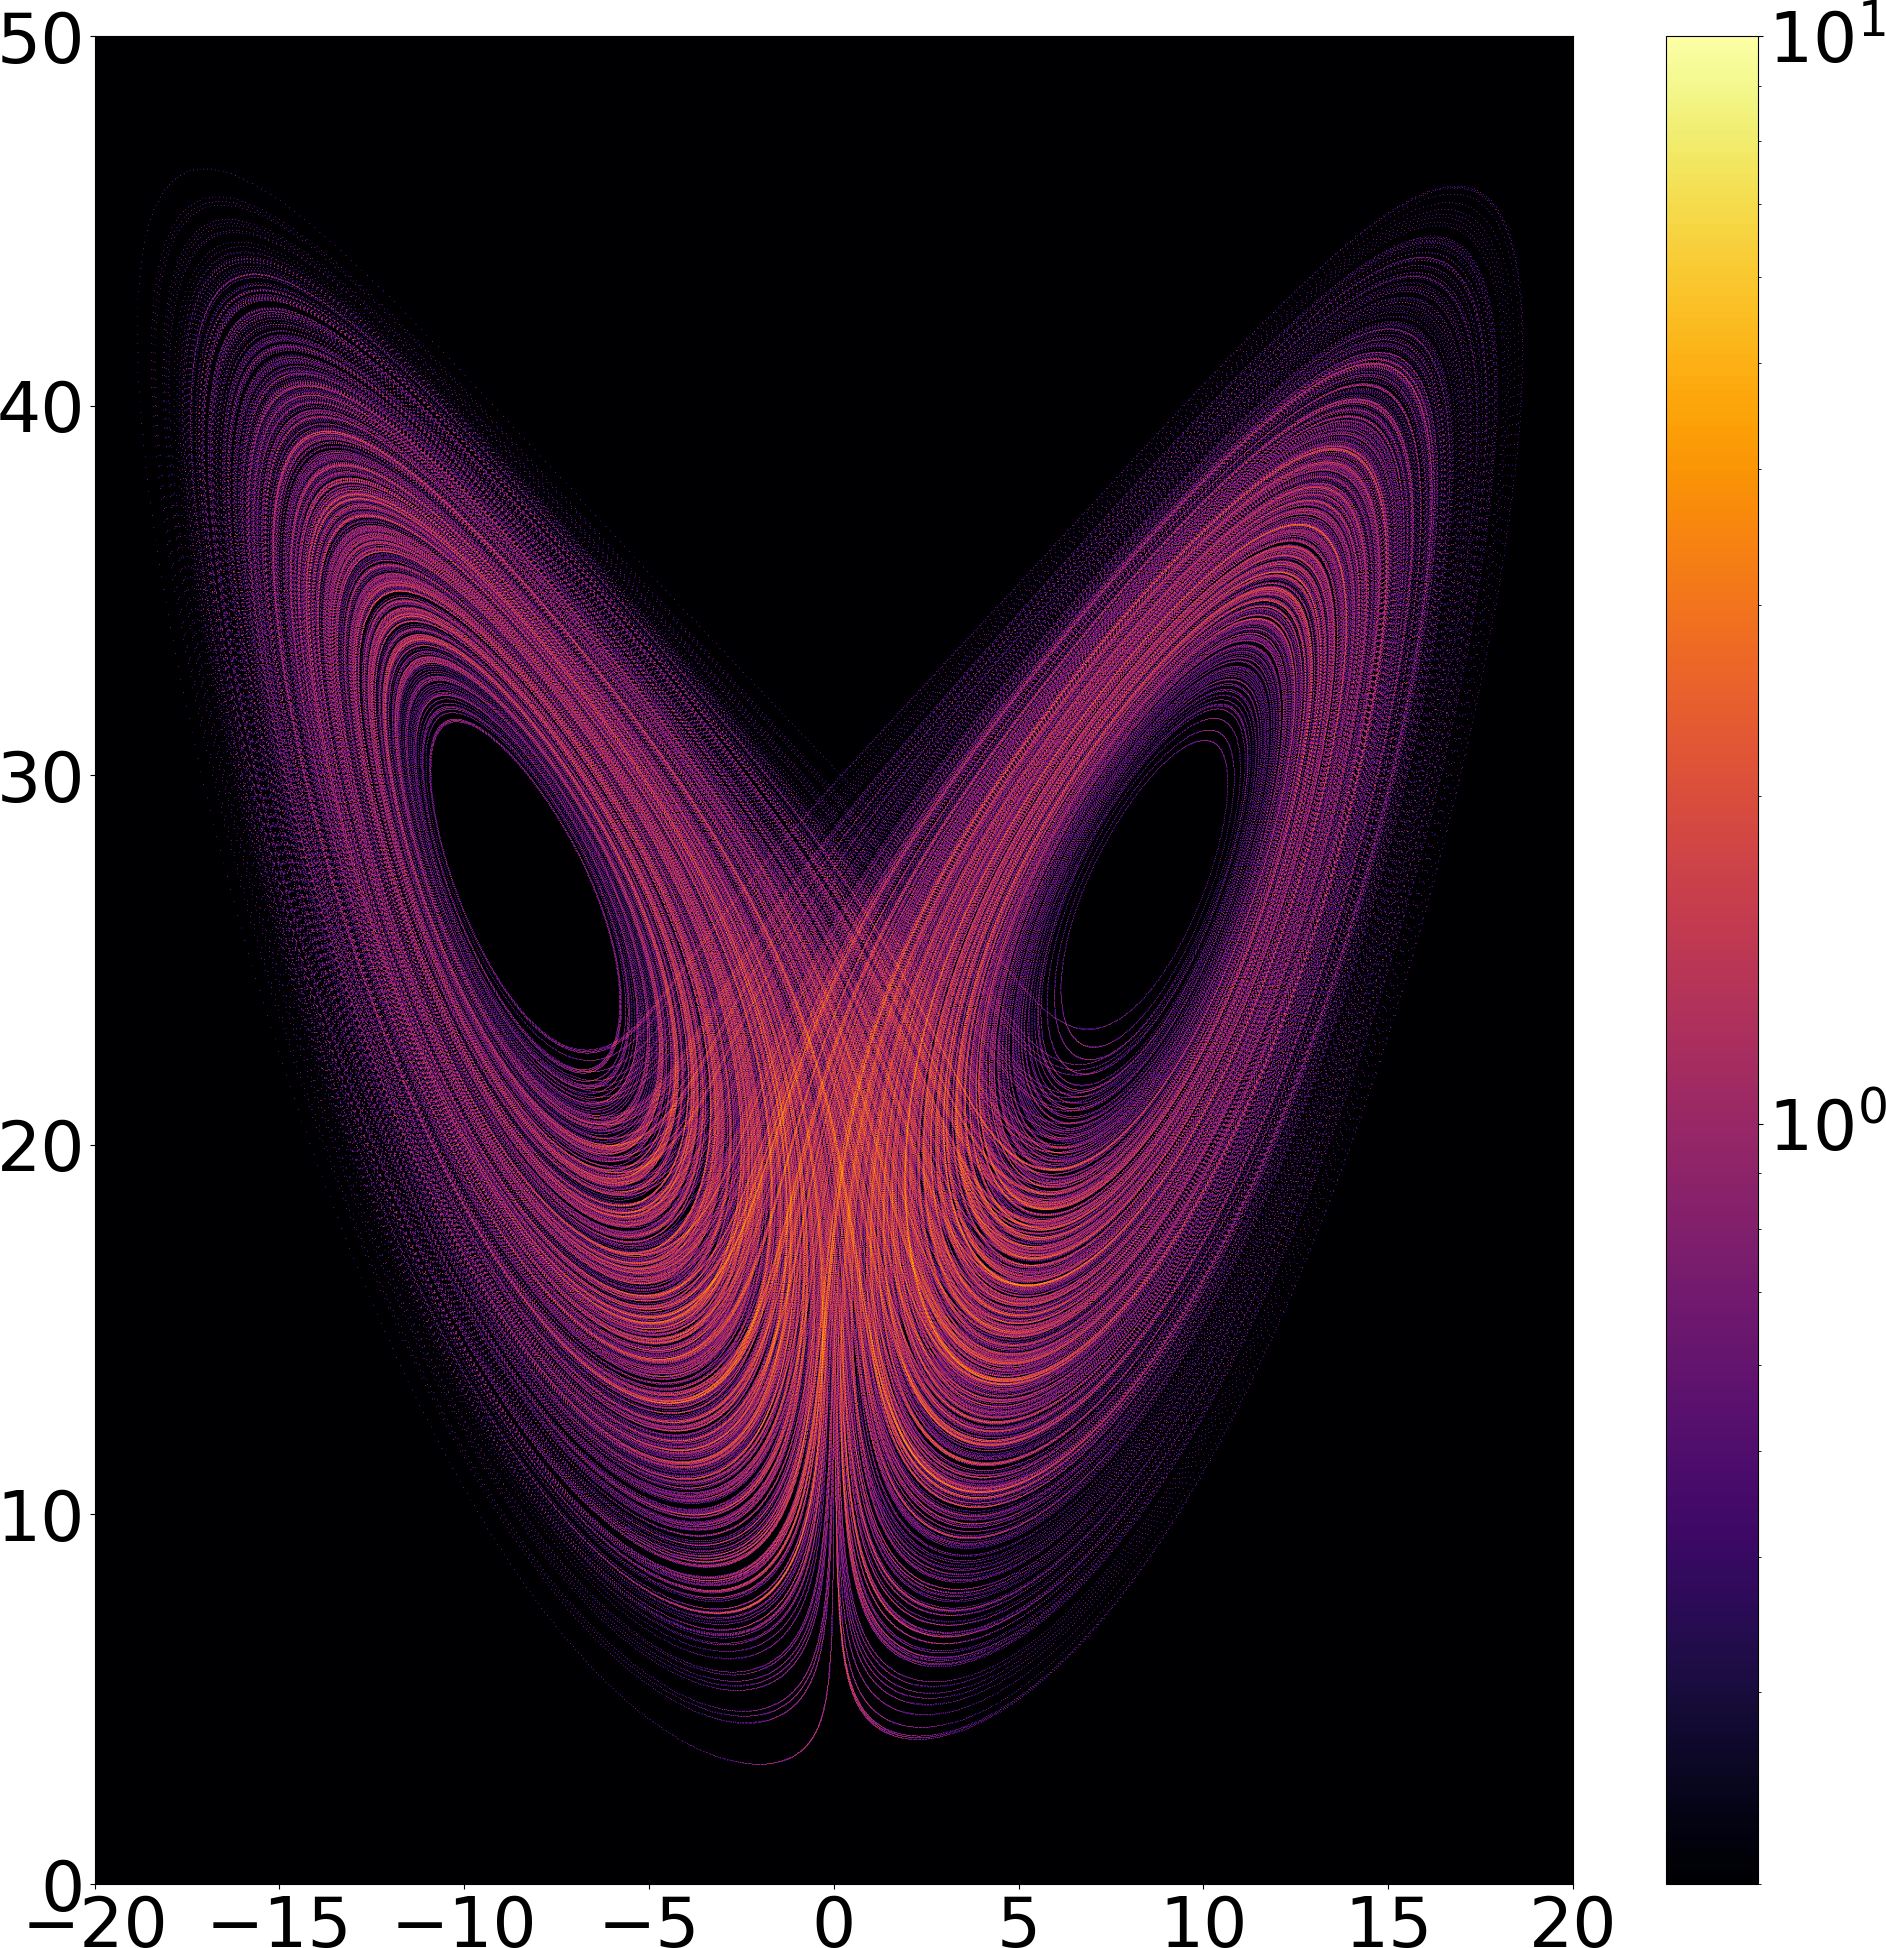
\includegraphics[width=0.48\textwidth]{figure/lorenz_trajectory_1000.0.png}
\hspace{0.02\textwidth}
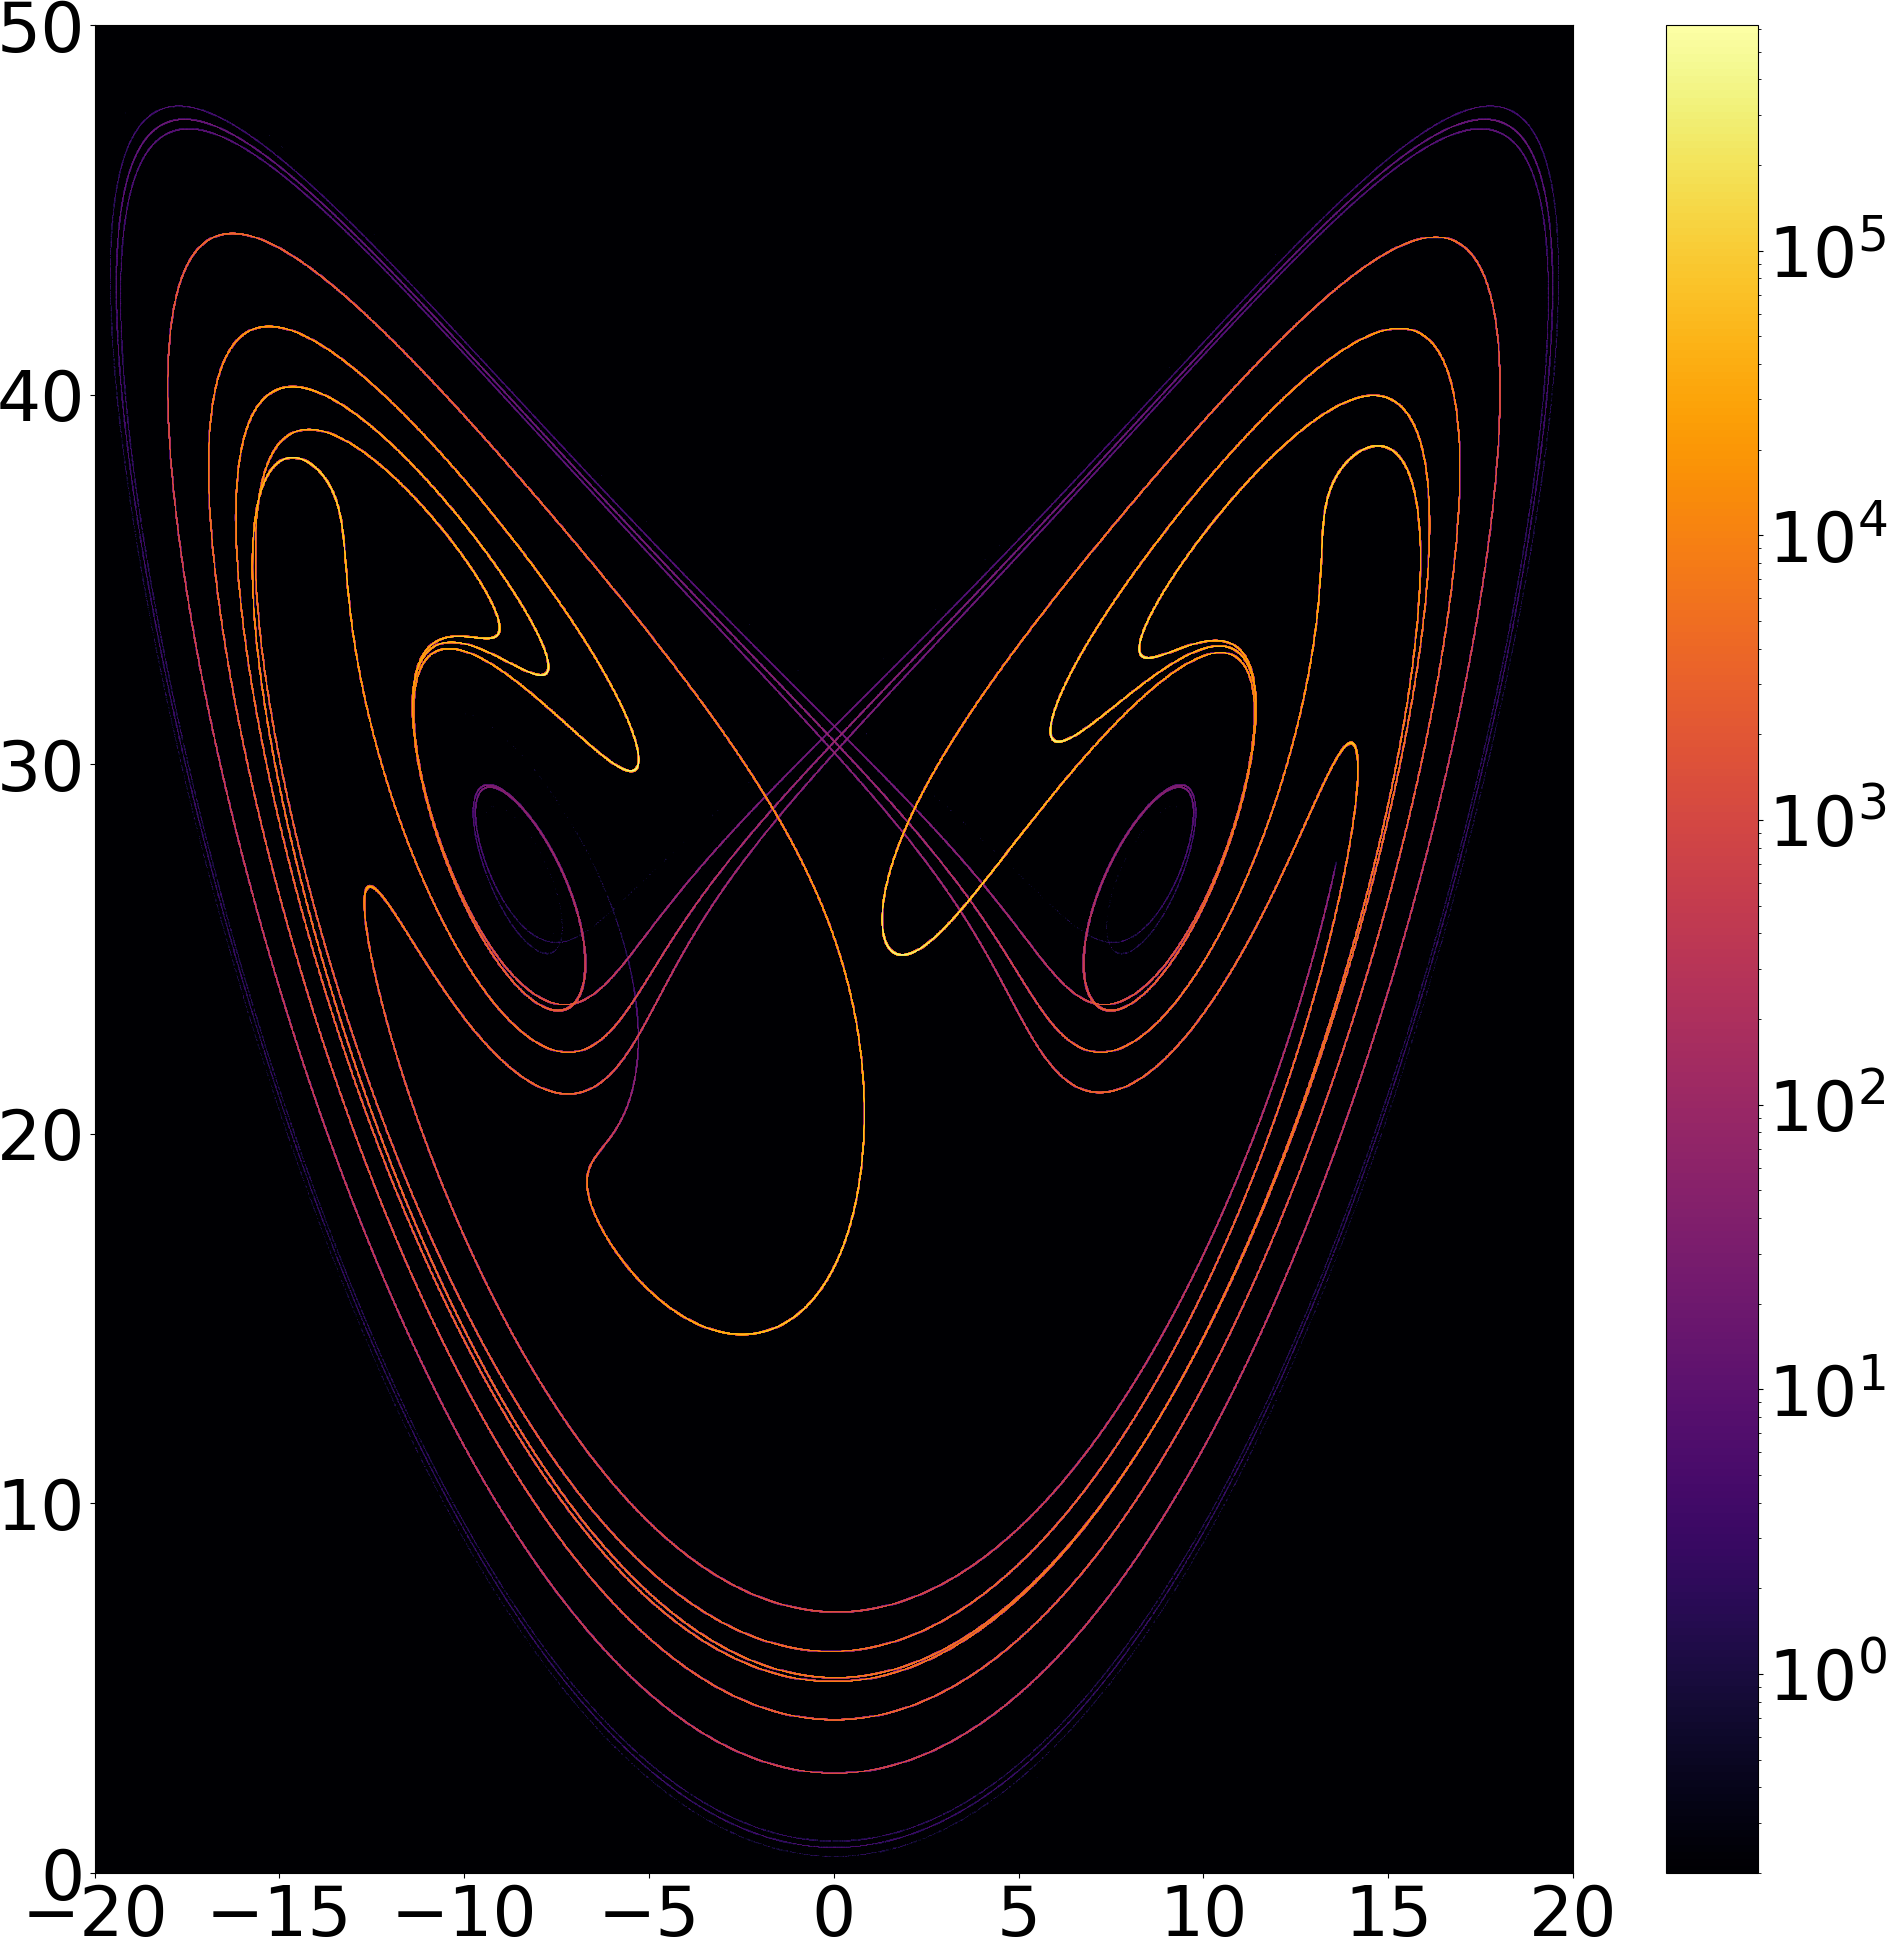
\includegraphics[width=0.48\textwidth]{figure/lorenz_ensemble_10.png}
\caption{
Left: An ensemble of initial conditions distributed uniformly in the box $u_1\in[0,1], u_2\in[0,1], u_3\in[28,39]$ 
after 10 time units of evolution, shown in in the $u_1-u_3$ plane.
Right: distribution of a trajectory of $1000$ time units in length.
In both plots, the color represent the number of samples in a
$2048\times2048$ uniform grid.  The trajectory is sampled every 0.001 time units.
}
\label{fig:lorenz_ergodicity1}
\end{figure}
\begin{figure}[H] \centering
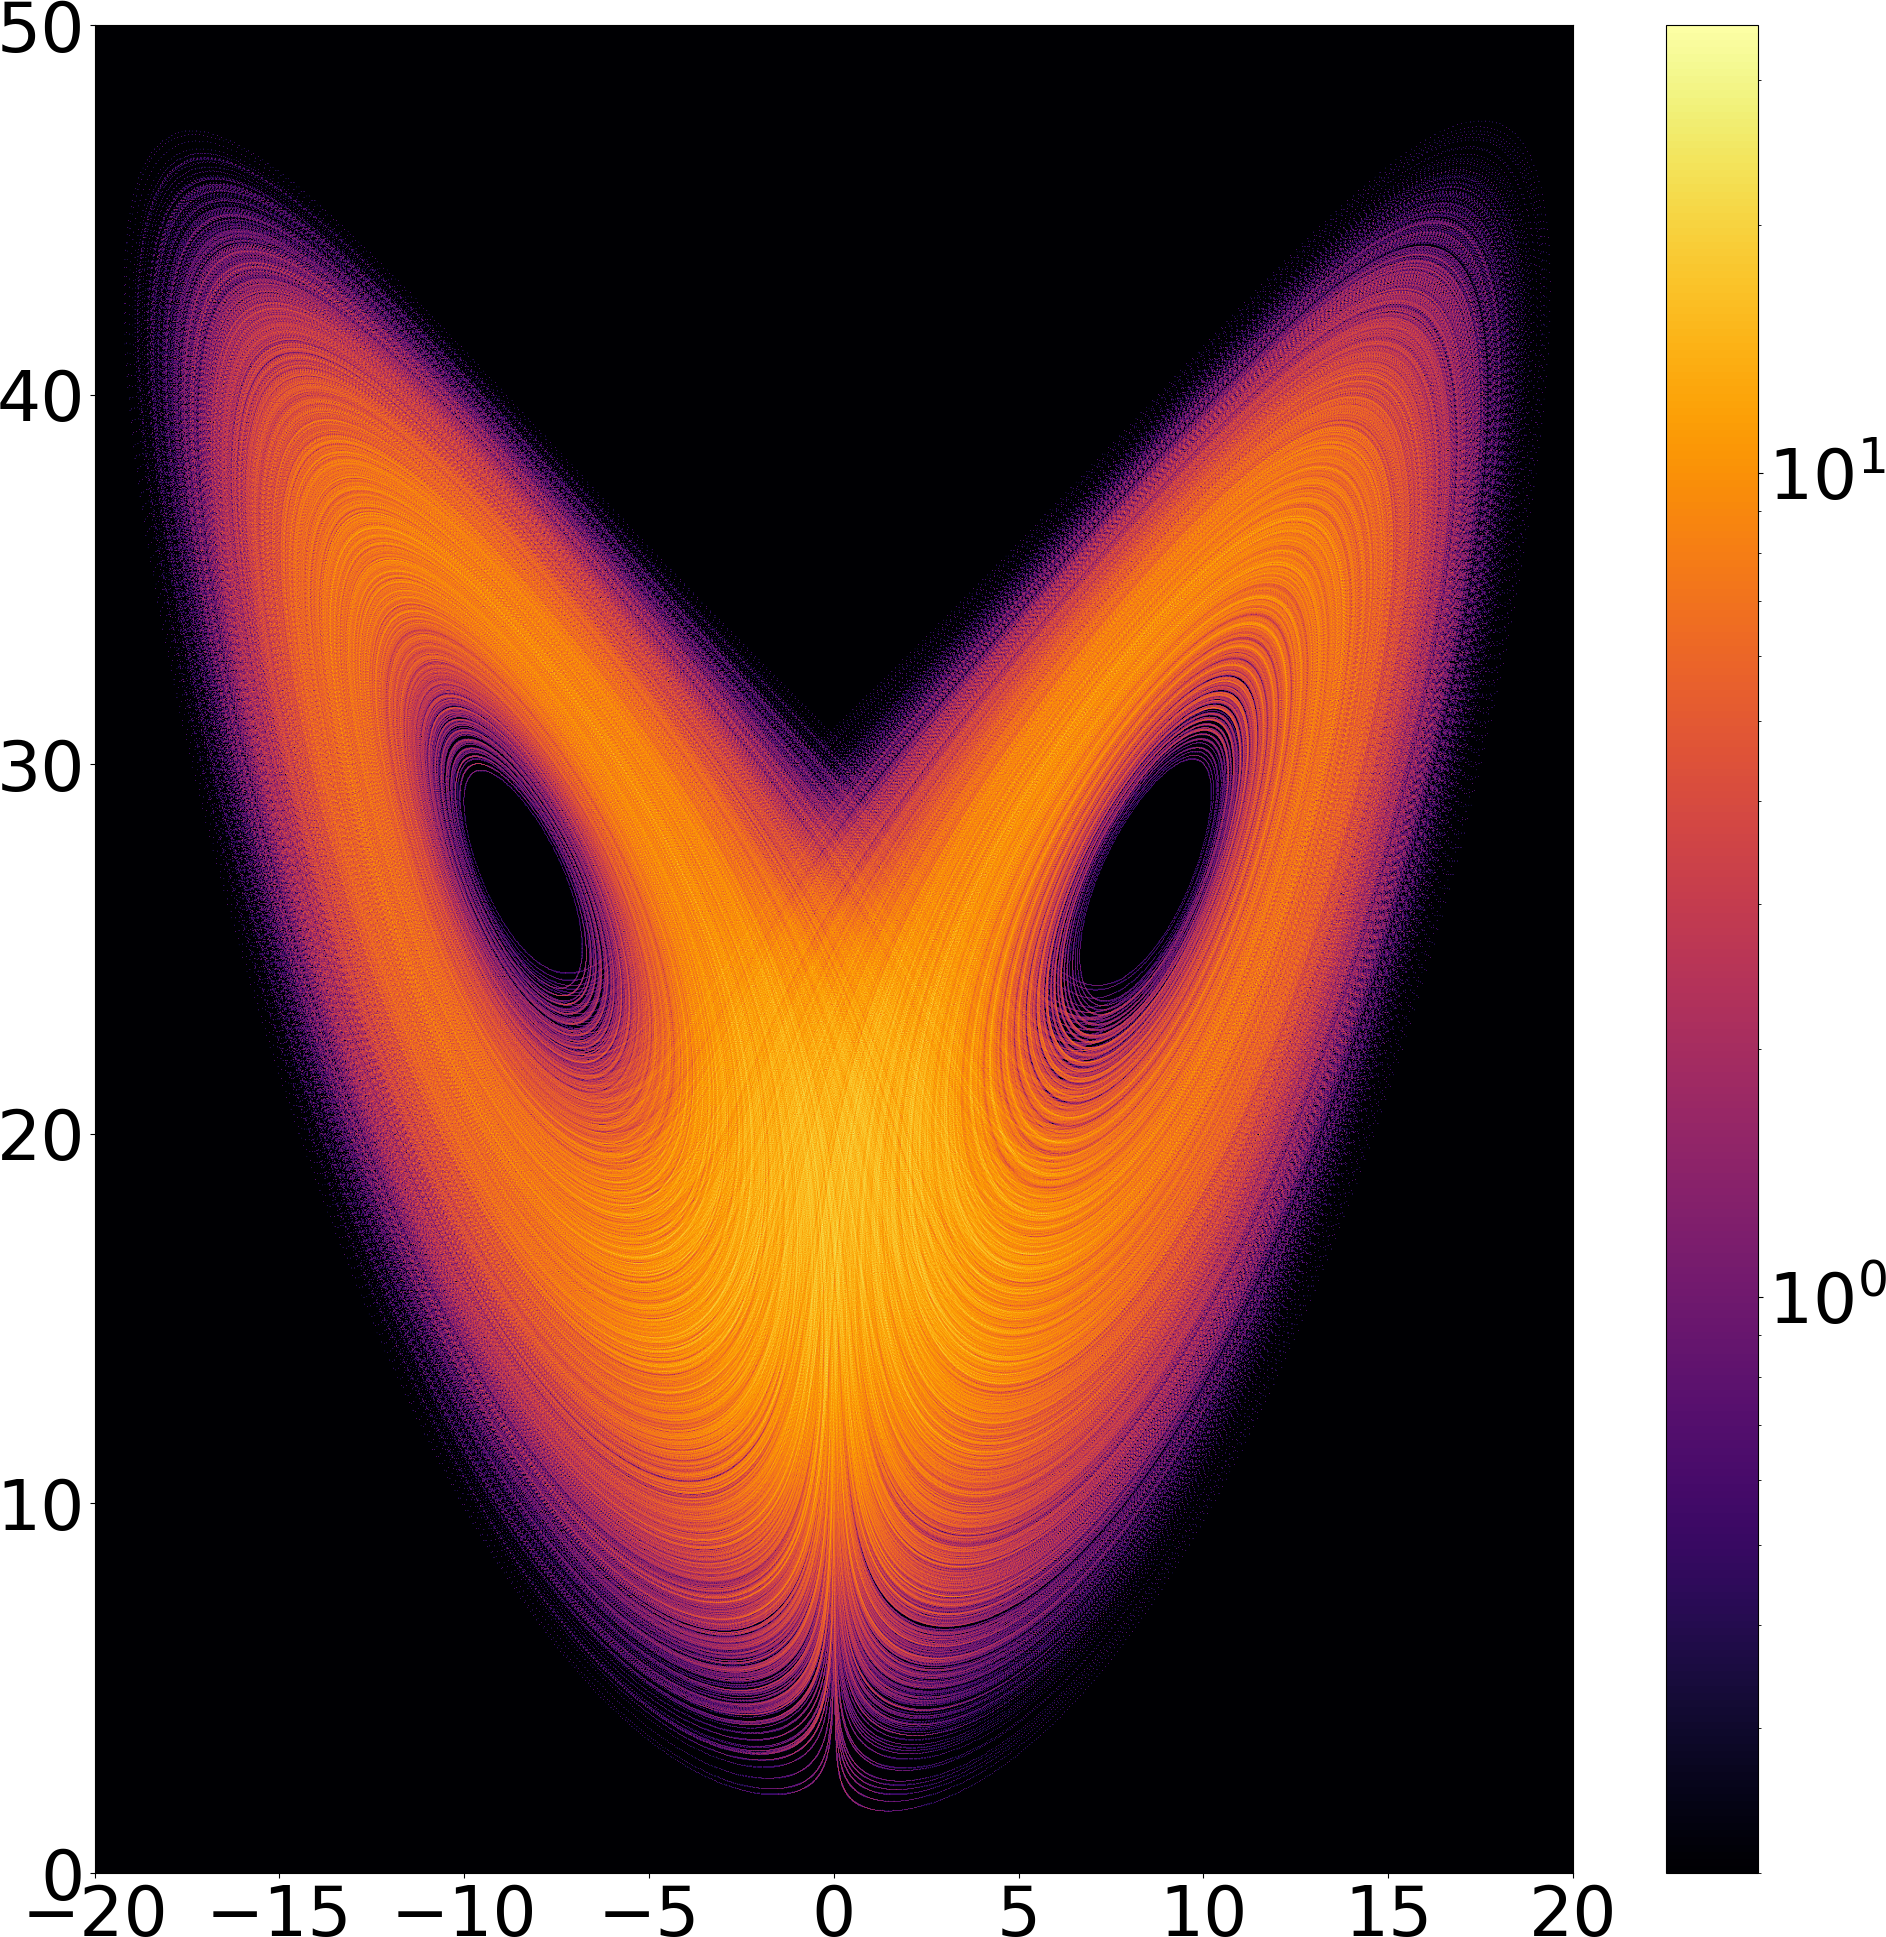
\includegraphics[width=0.48\textwidth]{figure/lorenz_trajectory_10000.0.png}
\hspace{0.02\textwidth}
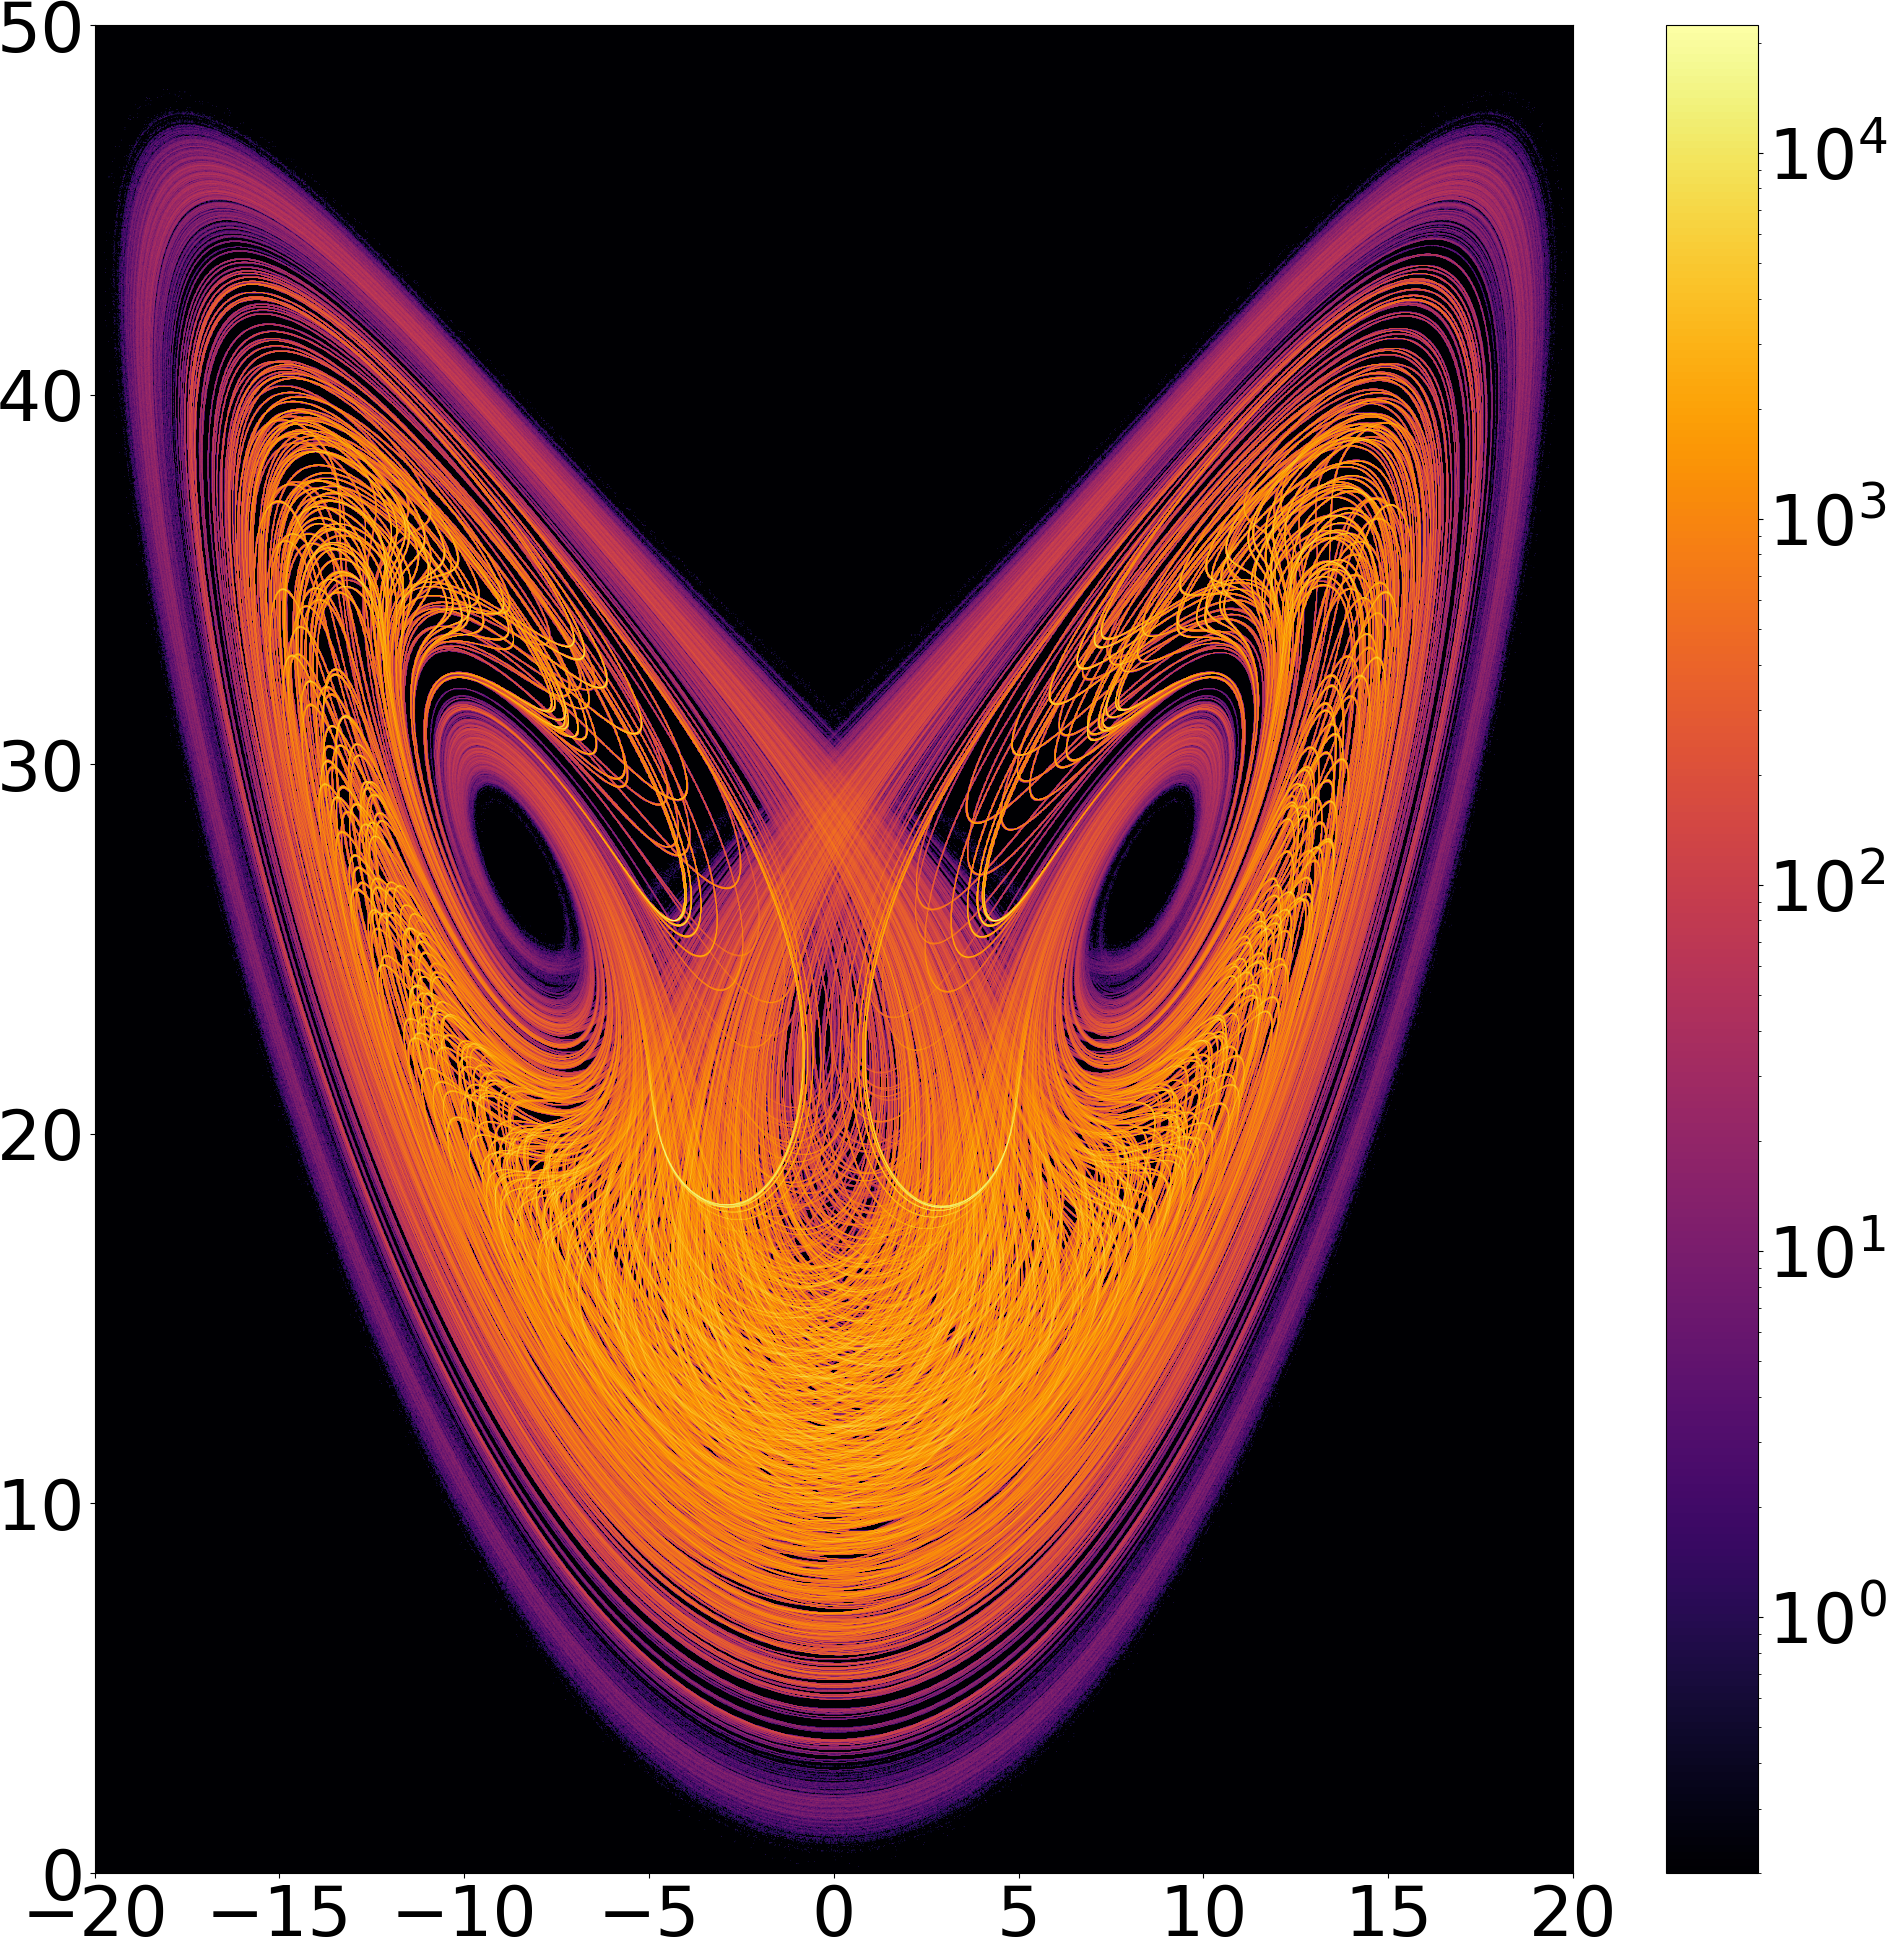
\includegraphics[width=0.48\textwidth]{figure/lorenz_ensemble_15.png}
\caption{
Left: distribution of the same ensemble as in Figure \ref{fig:lorenz_ergodicity1}
after another 5 time units of evolution.
Right: distribution of the same trajectory as in Figure \ref{fig:lorenz_ergodicity1}
evolved for $10,000$ time units.
}
\label{fig:lorenz_ergodicity2}
\end{figure}
\begin{figure}[H] \centering
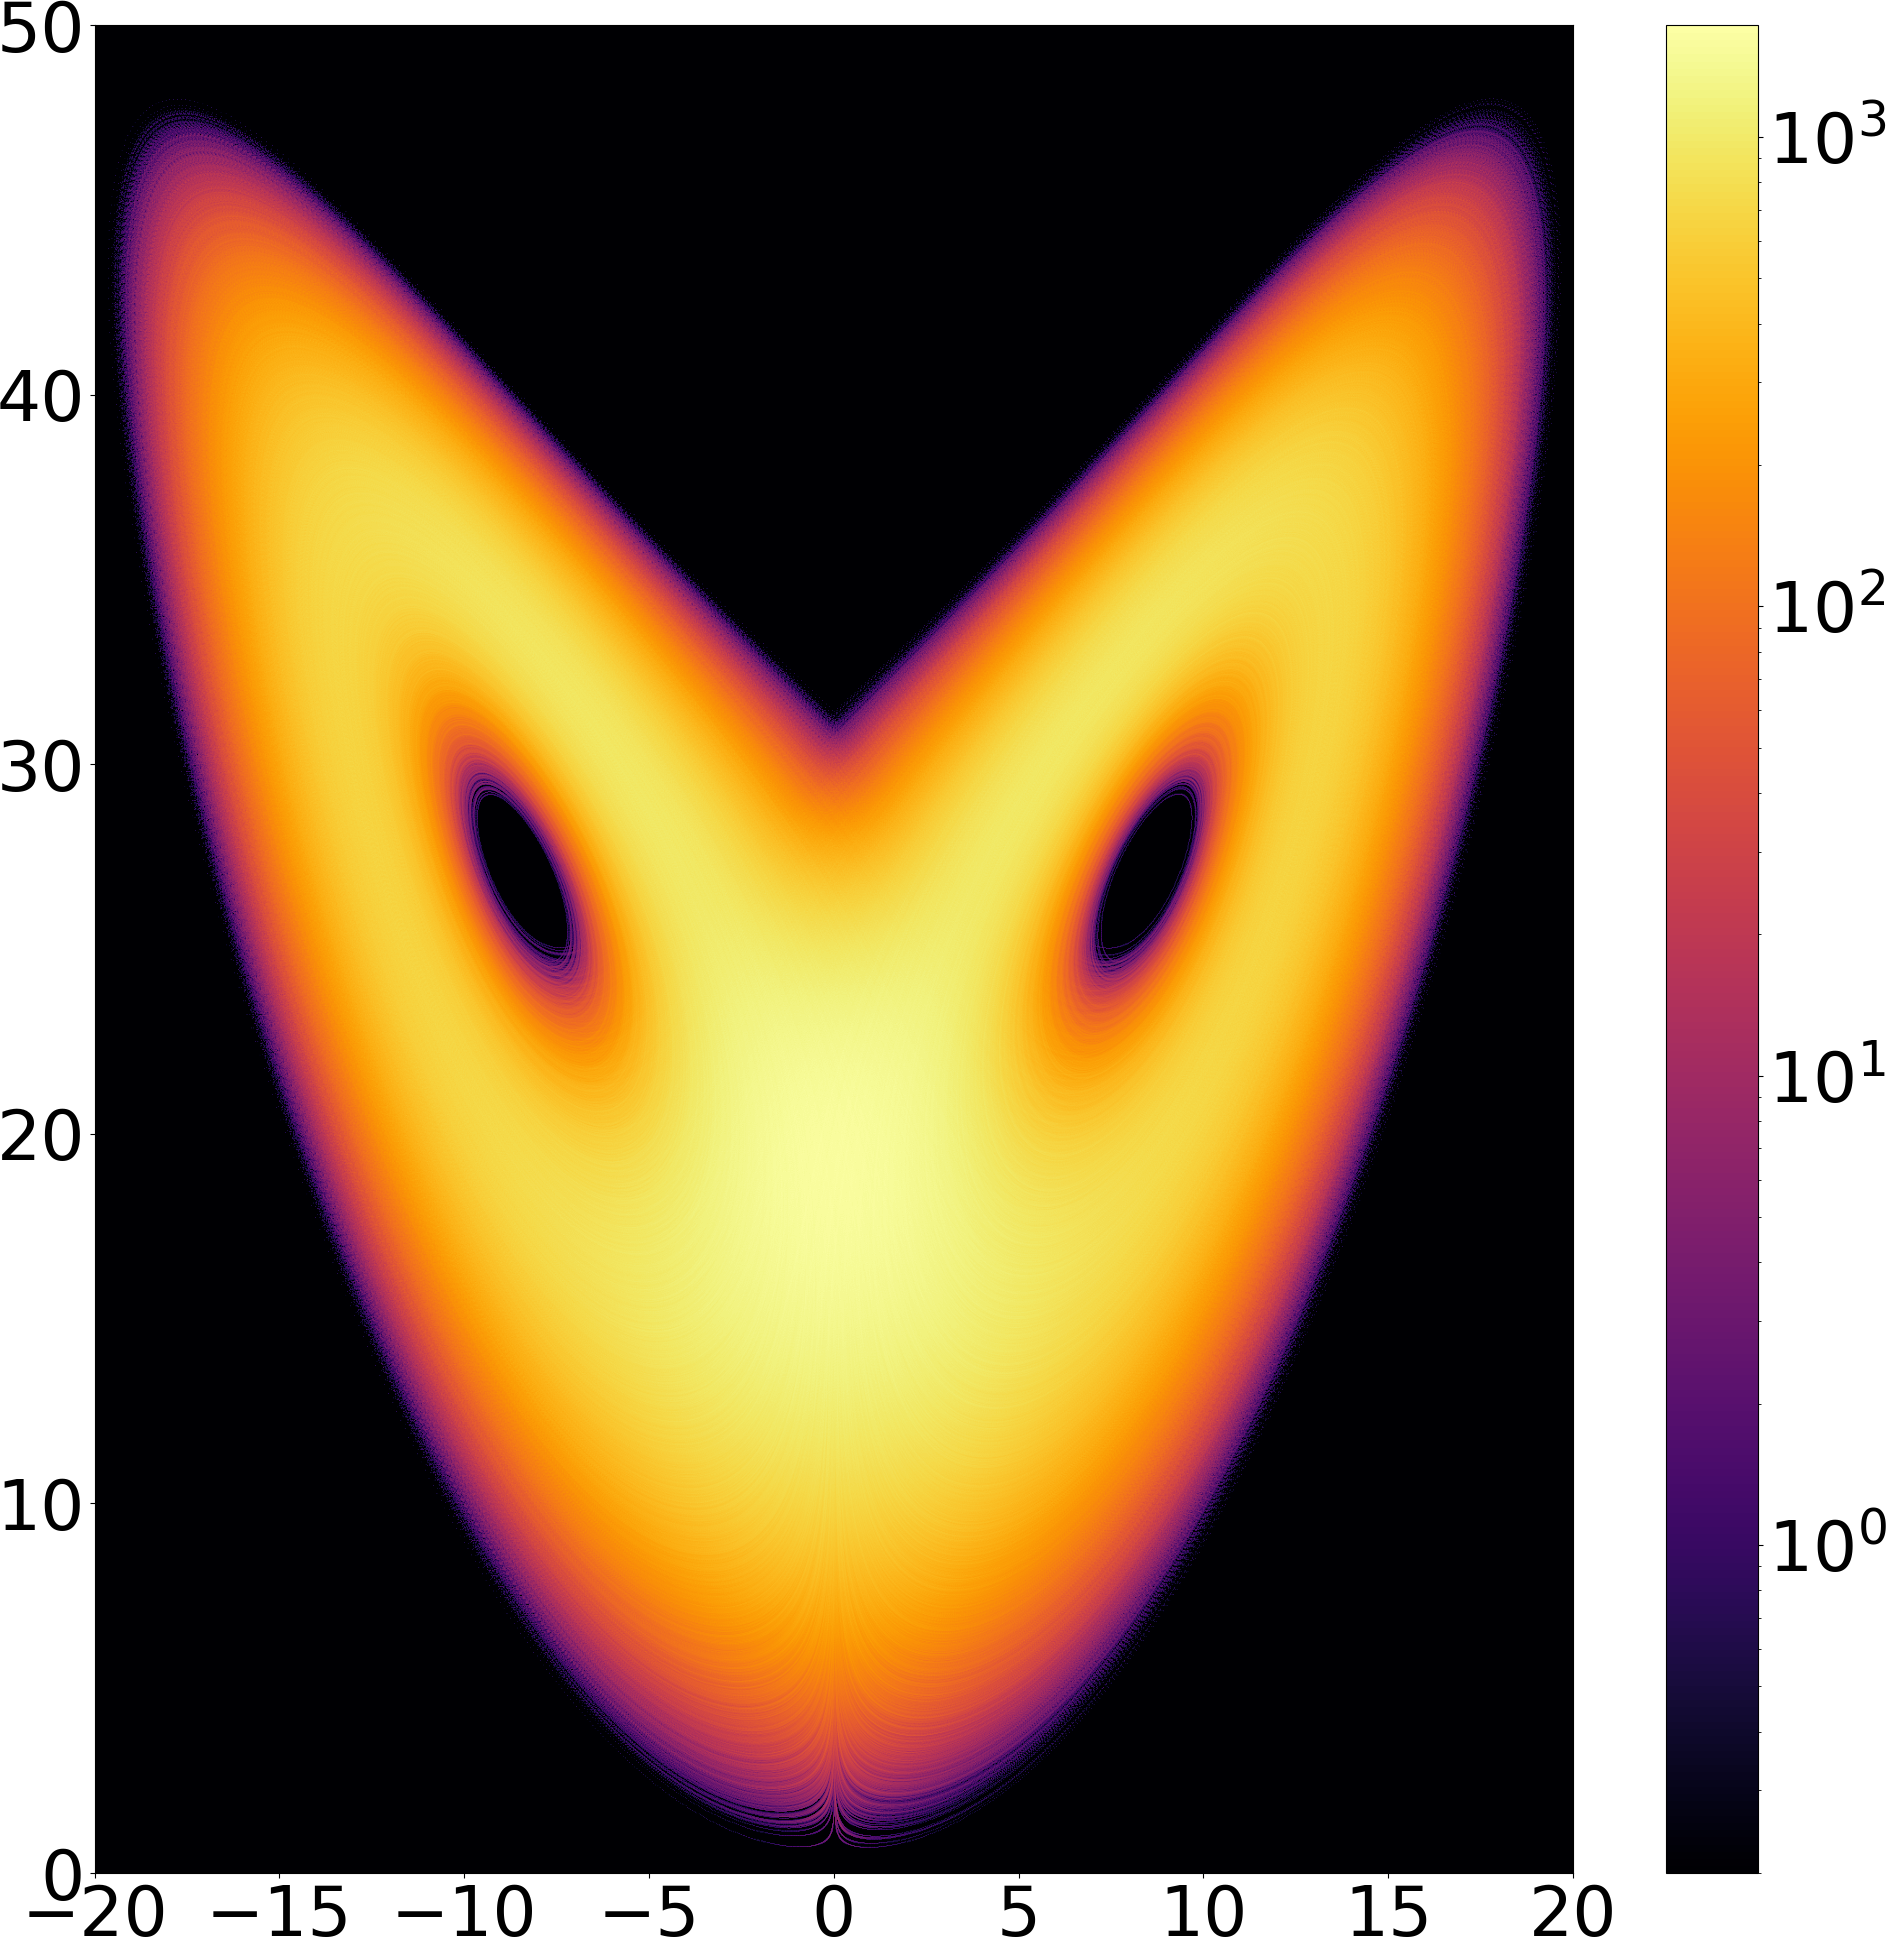
\includegraphics[width=0.48\textwidth]{figure/lorenz_trajectory_1000000.0.png}
\hspace{0.02\textwidth}
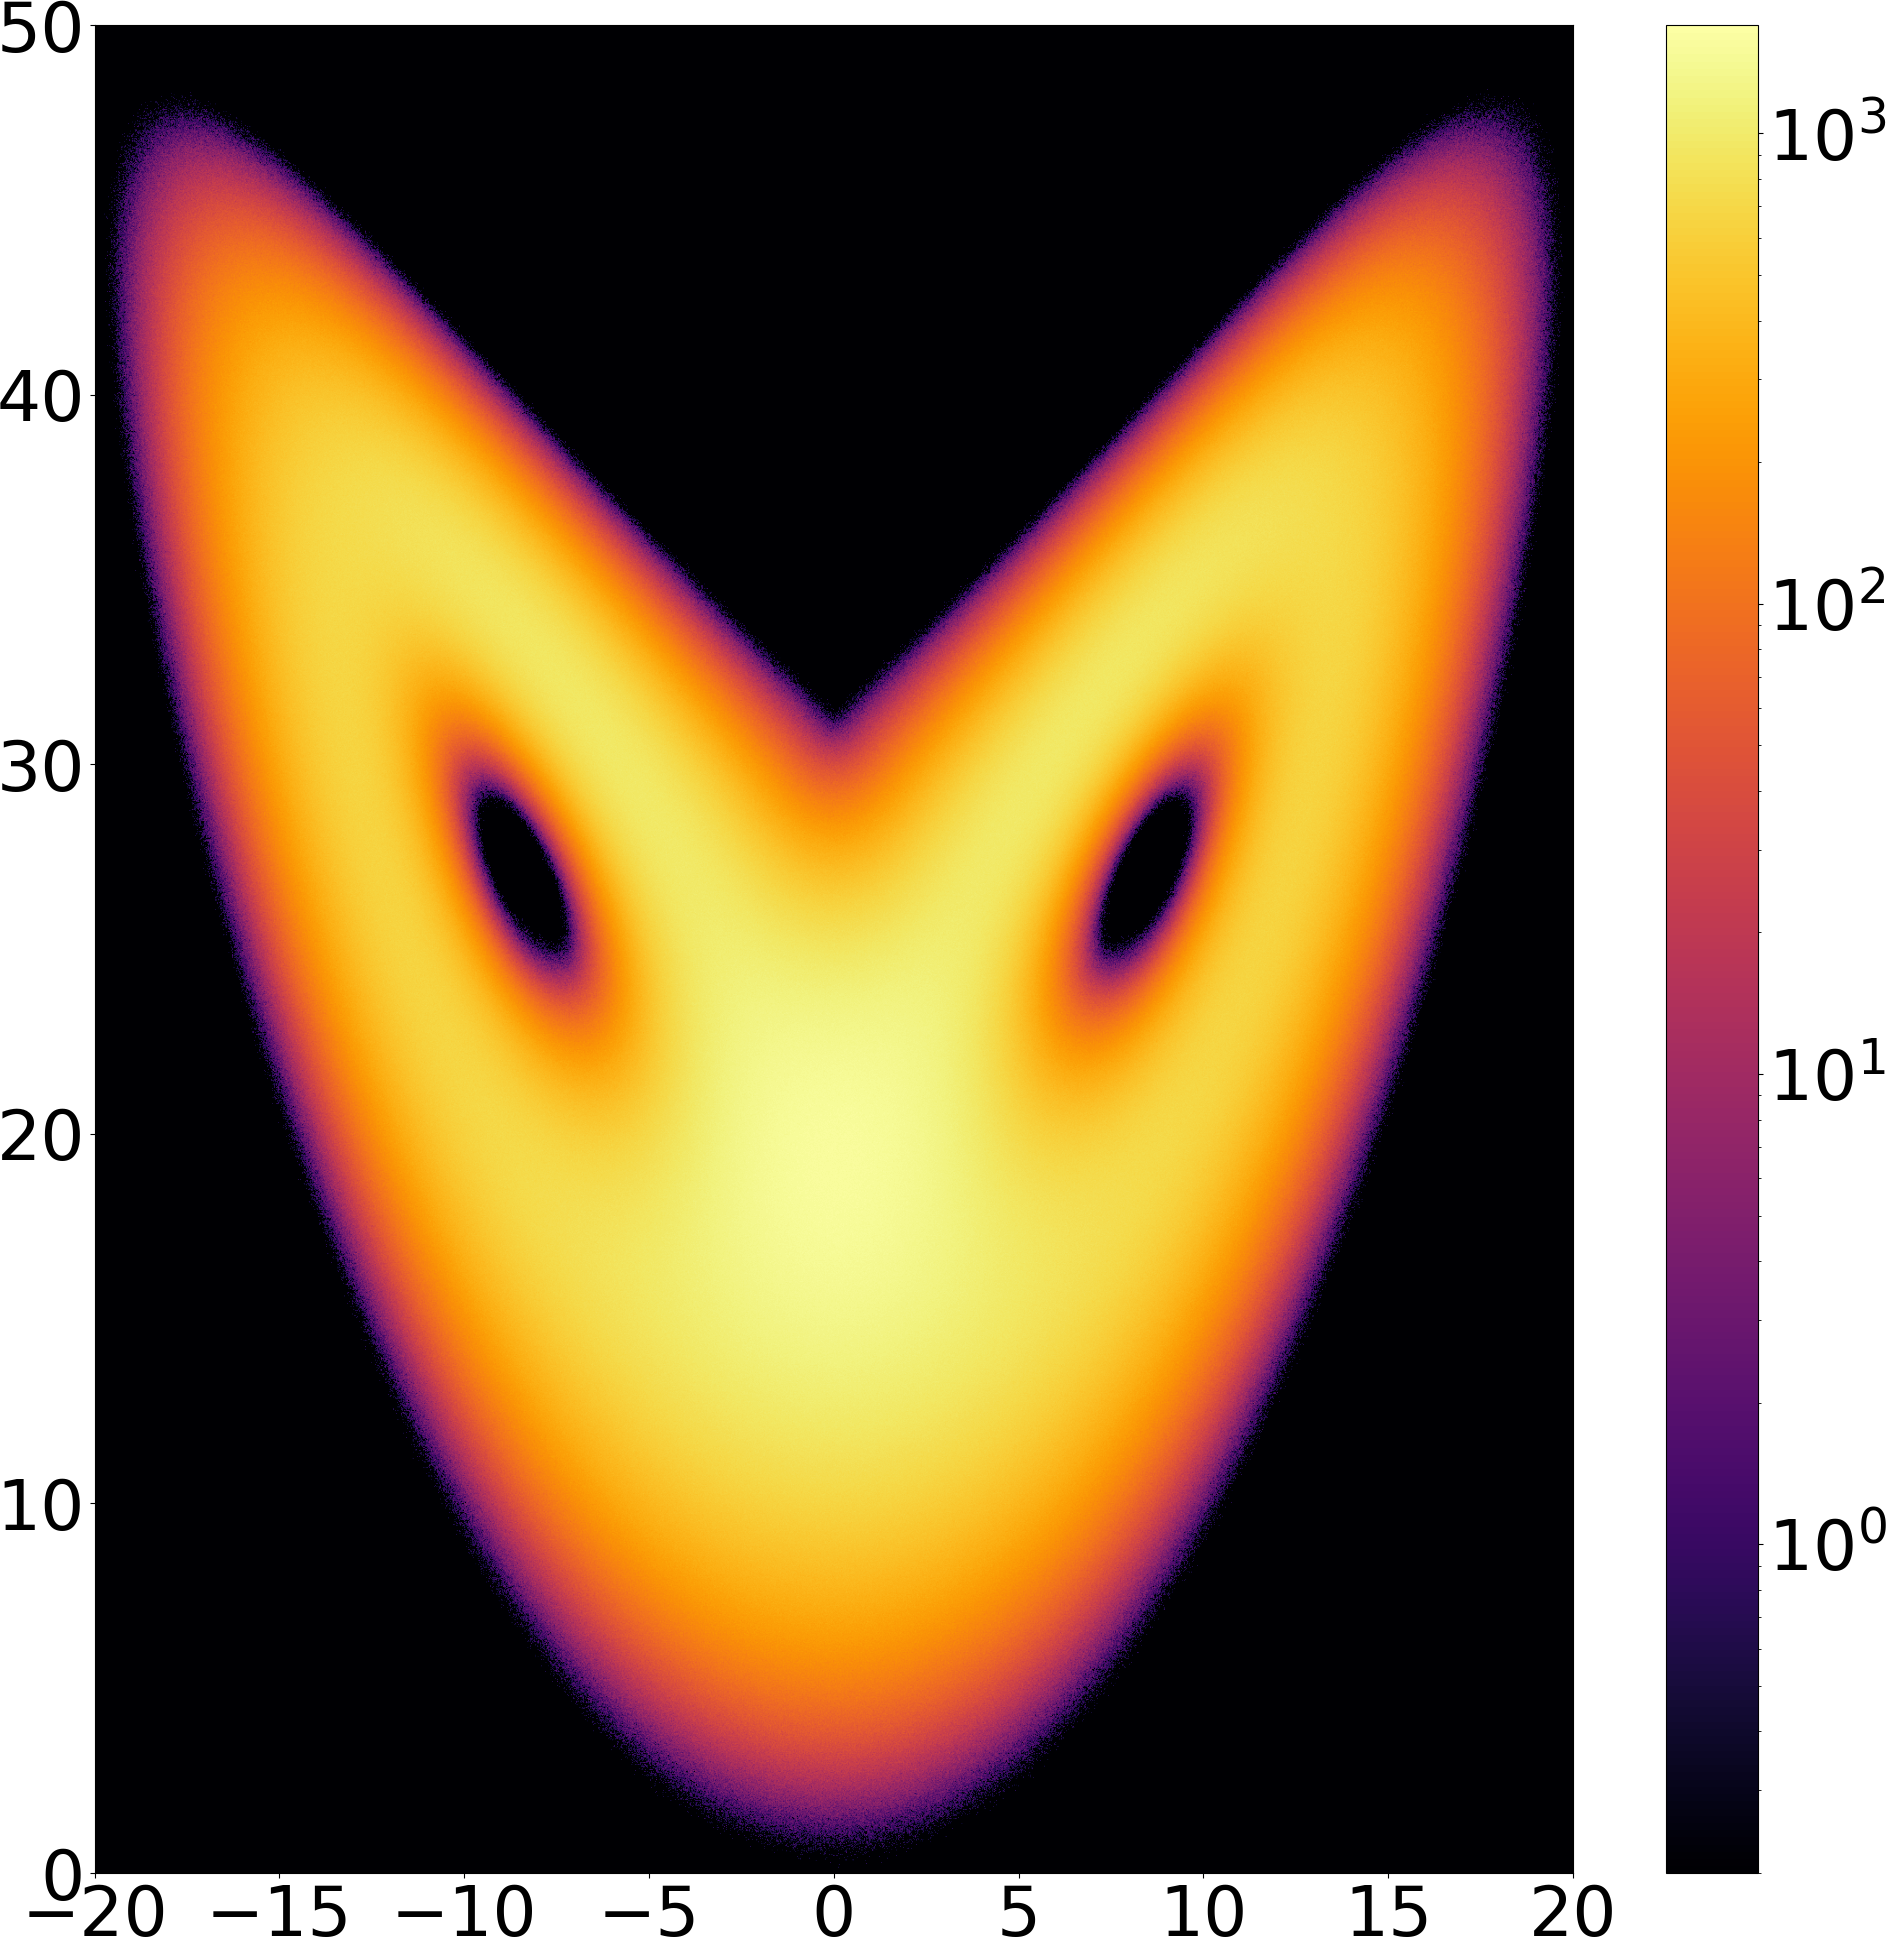
\includegraphics[width=0.48\textwidth]{figure/lorenz_ensemble_50.png}
\caption{
Left: distribution of the same ensemble as in Figures \ref{fig:lorenz_ergodicity1}
and \ref{fig:lorenz_ergodicity2} after a total of 50 time units of evolution.
Right: distribution of the same trajectory as in Figures \ref{fig:lorenz_ergodicity1}
and \ref{fig:lorenz_ergodicity2} evolved for $100,000$ time units.
}
\label{fig:lorenz_ergodicity3}
\end{figure}

The left column of Figures \ref{fig:lorenz_ergodicity1}-\ref{fig:lorenz_ergodicity3}
illustrates a physical solution of the Lorenz system,
\begin{equation}
\label{eqn:lorenz}
\frac{du}{dt} =
    \frac{d}{dt}\begin{pmatrix}u_1\\u_2\\u_3\end{pmatrix} =
    \begin{pmatrix}
        \sigma (u_2-u_1) \\
        u_1(\rho -u_3) - u_2 \\
        u_1\,u_2 - \beta\,u_3
\end{pmatrix}
\end{equation}
where $\sigma=10,\rho=28$, and $\beta=8/3$.  The solution starts at the initial
condition $u(0)=(0.01, 0.01, 28)$.  After a long time evolution, we observe that
the solution has visited a large portion of the $u_1-u_3$ plane with a varying, but well-defined, frequency.  We can use a probability distribution, $\mu$, to quantify
how frequently a physical solution visits portions the phase space.
Specifically, for a subset $A$ of the phase space, $\mu(A)$ measures the
fraction of time a very long physical solution spends inside the subset $A$.
With this distribution defined, the infinite-time average of any quantity $J(u)$ can be represented as an average of $J$ over the entire phase space $U$, weighted
by this statistical distribution $\mu$.  Mathematically,
\begin{equation}
    \frac1T \int_0^T J(u(t))\,dt \xrightarrow{T\to\infty}
    \int_U J(u)\: d\mu(u)
\end{equation}

Remarkably, the distribution $\mu$ not only characterizes the history of
a long physical solution, but also describes the settled state of
an ensemble of solutions.
This is illustrated on the right column of Figures \ref{fig:lorenz_ergodicity1}--\ref{fig:lorenz_ergodicity3}.
We generate these plots by starting from an ensemble of about one billion initial
conditions, randomly and uniformly spaced in a small three-dimensional box.  All these billion solutions are evolved by solving Eq. \ref{eqn:lorenz} for 10, 15, and 50 time units, to obtain the plots. 
We observe that, as time evolves, the ensemble spreads over an increasingly
larger portion of the $u_1-u_3$ plane. After a long time, the ensemble settles into a set known as an \emph{attractor} that does not change with time, and contains the \emph{unstable manifold}, which appears as filaments forming the attractor. The distribution of the ensemble on the attractor becomes identical to the distribution of a single, very long physical
solution, which is also contained in the attractor (Figure \ref{fig:lorenz_ergodicity3}).

This remarkable agreement has been thoroughly studied under the subject
of ergodic theory. Under surprisingly weak conditions, a solution starting from
{\bf almost} any initial condition, chosen randomly from a set enclosing the attractor, is a physical solution \cite{young}.   
Meanwhile, an ensemble of trajectories starting from any distribution with a 
finite density also evolves towards the same final distribution, $\mu$. Due to expansion of a volume of solutions tangent to the attractor filaments, a finite density under long-time evolution becomes absolutely continuous on the unstable manifold, i.e., the likelihood of a trajectory visiting any set not intersecting the attractor filaments is zero. The 
stationary distribution achieved on long-time evolution of the ensemble that has the absolute continuity property is called the Sinai-Ruelle-Bowen
(SRB) measure. The absolute continuity property is sufficient to ensure that the SRB measure is the same $\mu.$ That is, the SRB measure is physically observed in the sense that  
\nisha{what do we mean by ``under sufficient regularity conditions'' here? Suggesting a modification to the previous sentence} physical solutions produce long-time-averages which are expectations with respect to the SRB measure. 

Note that almost any, not any, initial condition leads to a physical solution. A set of special initial conditions
contained in a neighborhood of the attractor may exist starting from which physical solutions are not generated. These initial conditions do not produce the same statistics as the physical solutions. This special set of initial conditions is Lebesgue measure zero -- one
has zero chance of finding such an initial condition by randomly sampling.
Nonphysical solutions thus take an effort to find.  Nevertheless, they
turn out to be important when discussing shadowing, the topic of this paper.
We first introduce a type of obviously nonphysical solutions in the next
subsection, before discussing a less obvious type in Section \ref{sec:quasiphysical}.

\subsection{Nonphysical solutions Type I: Periodic Solutions}

A periodic solution is nonphysical because it 
does not visit as much
of the phase space as a physical solution does.
Figure \ref{fig:lorenz_periodic} shows
a few periodic solutions of the Lorenz equation. Comparing these solutions
to the physical solution visualized in Figures \ref{fig:lorenz_ergodicity1}--\ref{fig:lorenz_ergodicity3},
we see that the periodic solutions are significantly more limited in their
extent of exploration.

\begin{figure}[H]\centering
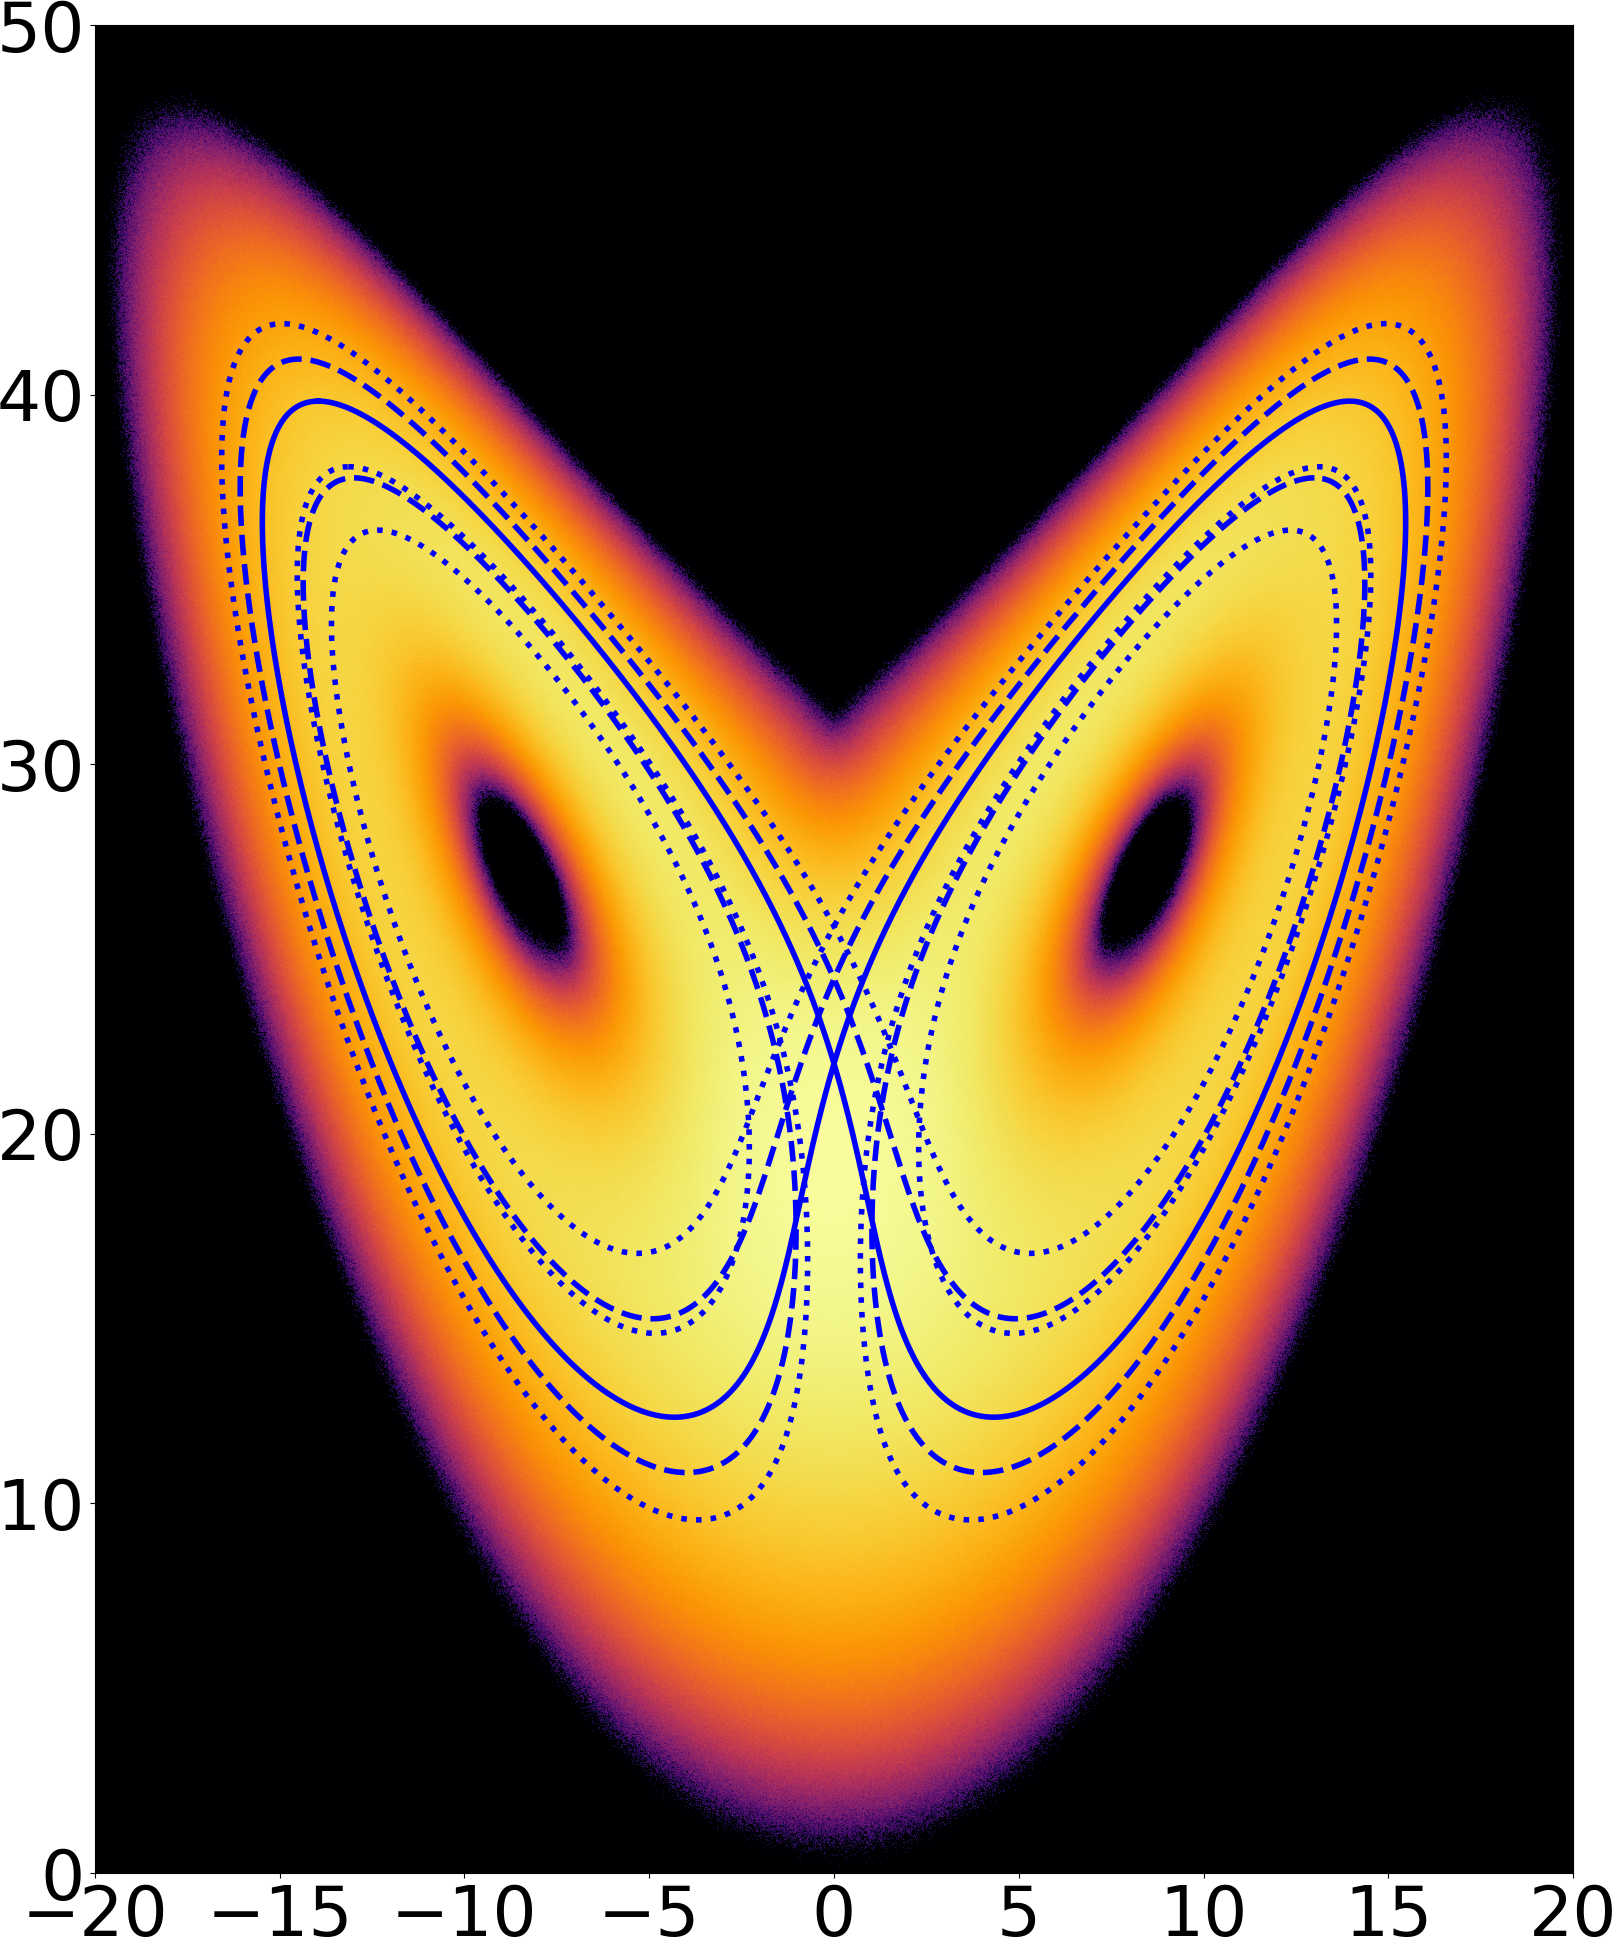
\includegraphics[width=0.48\textwidth]{figure/lorenz_periodic.png}
\caption{Periodic solutions of the Lorenz equation, overlaid on top of
its SRB distribution.  The solid line, dashed line, and dotted line
represent three distinct periodic solutions.}
\label{fig:lorenz_periodic}
\end{figure}

Because periodic solutions have a more limited extent in the phase space, their
statistics are different from physical solutions.
Here we illustrate the difference using the mean of two
quantities of interest
\begin{align}
    J_1(u) = u_3\;,\quad J_2(u) = e^{-\dfrac{u_3^2}2}.
\end{align}
Table \ref{tab:lorenz_periodic_stats} shows these quantities
of interest averaged over the three periodic solutions shown in Figure
\ref{fig:lorenz_periodic}, compared against those averaged over a
physical solution.  Here, Periodic \#1, \#2, and \#3 correspond to
the solid, dashed, and dotted lines, respectively.
We observe from the table that although the mean of $J_1$ over the periodic
solutions are different but comparable to the mean over physical solutions.  The mean of $J_2$ over the periodic solutions, on the other hand,
is orders of magnitude different from that of the physical solutions.
These differences disqualify the periodic solutions from being physical.
\begin{table}[H]
    \centering
    \begin{tabular}{c|c|c|c|c}
             & Periodic \#1 & Periodic \#2
             & Periodic \#3 & Physical solutions \\
    \hline
        $J_1$& 23.05 &
               23.19 &
               23.37 &
               23.67 \\
        $J_2$&$4\times 10^{-35}$&
              $7\times 10^{-28}$&
              $3\times 10^{-22}$&
              $1.58\times 10^{-05}$
    \end{tabular}
    \caption{Comparison of statistics computed from periodic solutions of the Lorenz equation with the statistics computed from physical solutions}
    \label{tab:lorenz_periodic_stats}
\end{table}

While periodic solutions are generally difficult to find,
the Lorenz equation has a special feature that makes the task significantly
easier.  In a typical solution to the Lorenz equation, the 
$u_3(t)$ component oscillates in a pattern that appears neither regular nor random.  Lorenz
observed that the height of one peak in the oscillation can predict the height of the next peak.  He quantified his observation by the Lorenz map,
as shown in Figure \ref{fig:lorenz_map}.

\begin{figure}[H]\centering
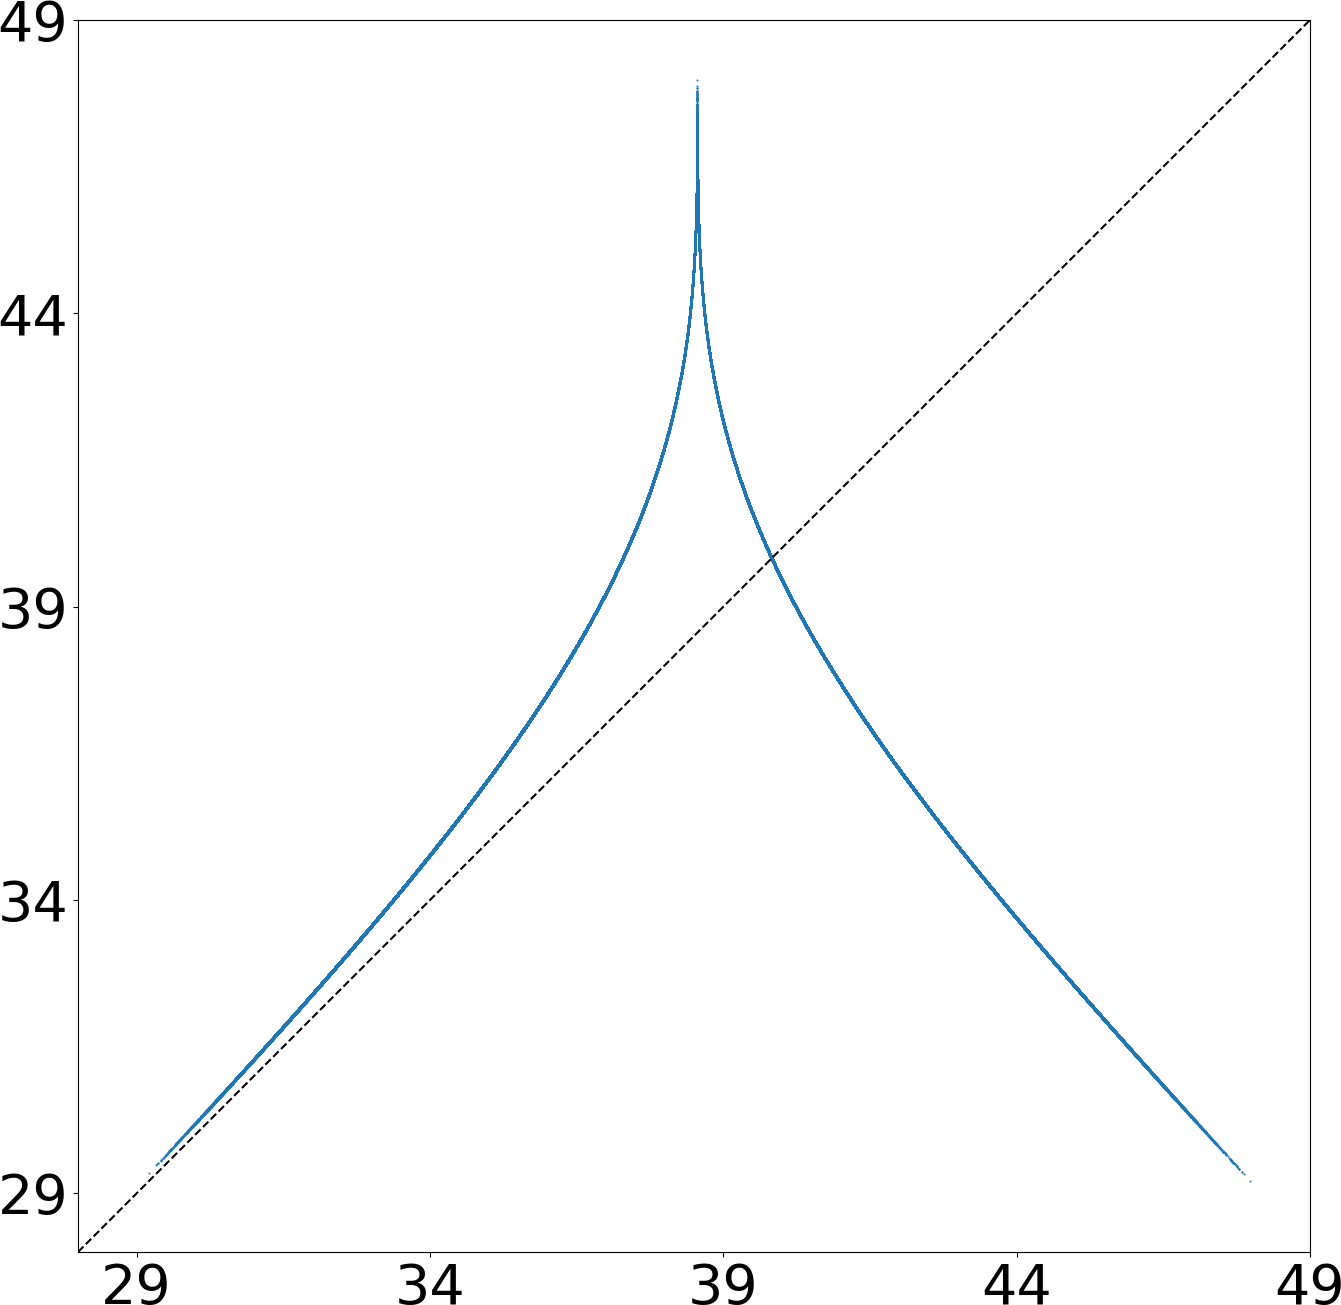
\includegraphics[width=0.48\textwidth]{figure/lorenz_zmax_10_28_2.6666666666666665.png}
\hspace{0.02\textwidth}
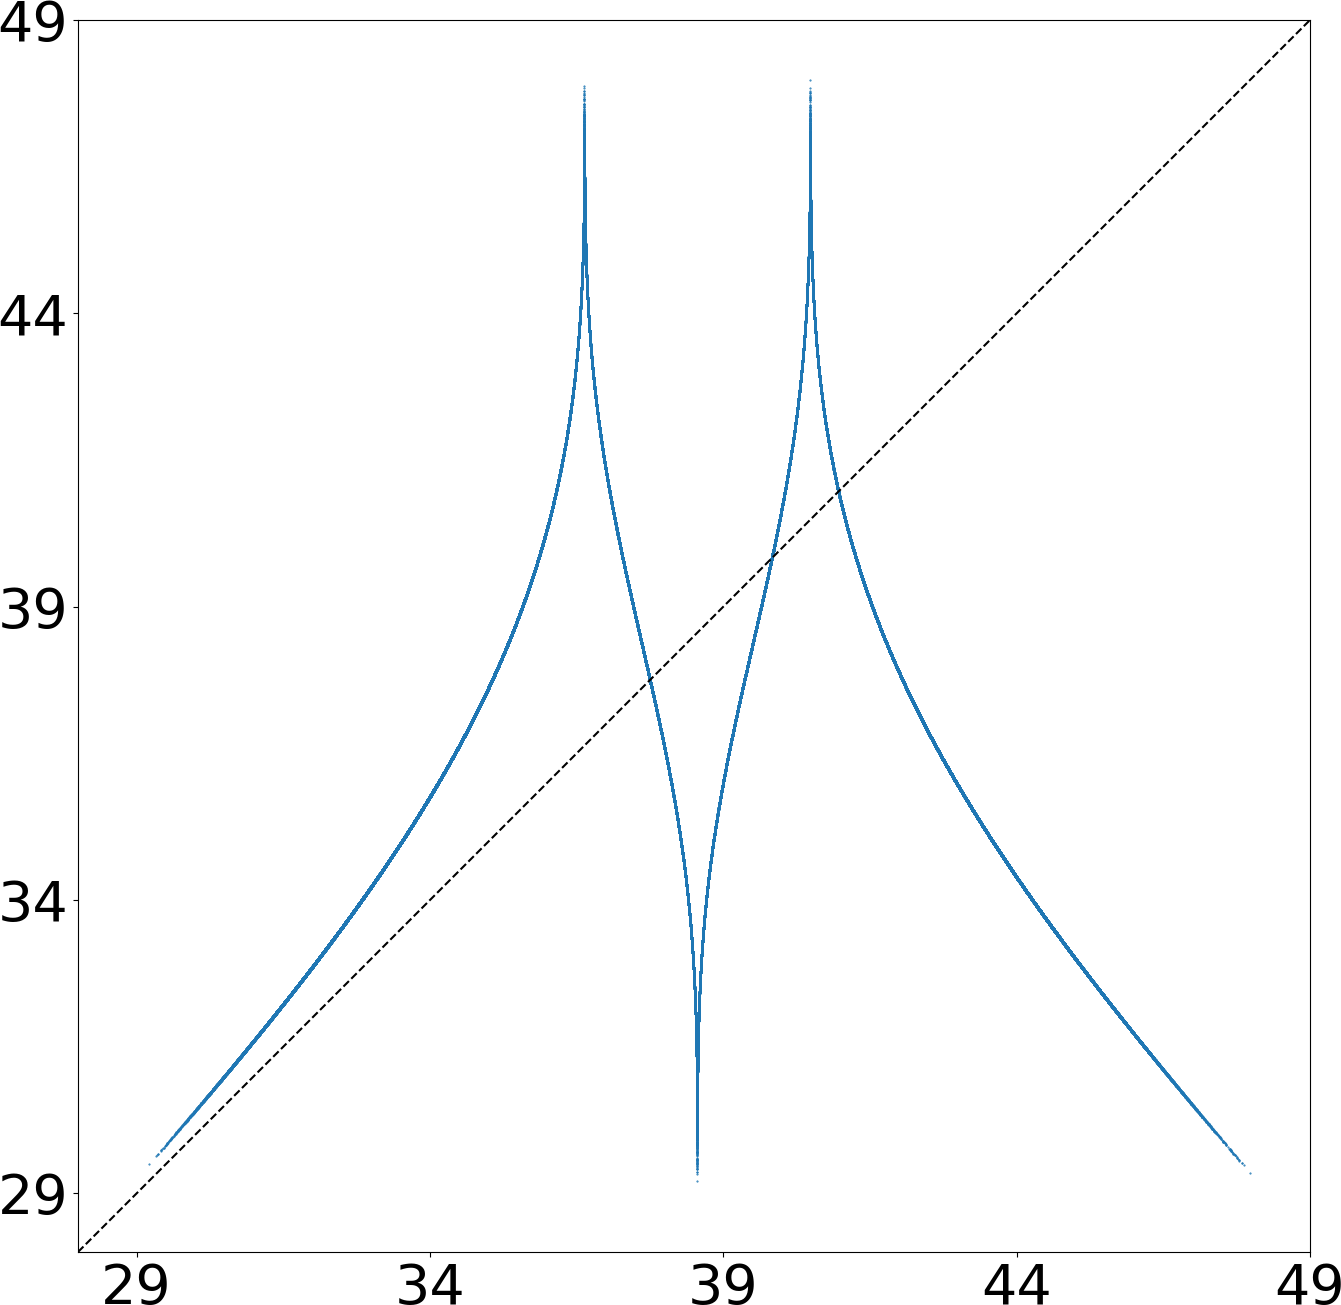
\includegraphics[width=0.48\textwidth]{figure/lorenz_zmax2_10_28_2.6666666666666665.png}
\caption{Left: the Lorenz map.  The x-axis is the $n$-th local maximum of $u_3(t)$ over a
long solution; the y-axis is the $(n+1)$-th local maximum of $u_3(t)$.  The intersection of this curve
with the diagonal dashed line indicates the initial condition for the solid line
in Figure \ref{fig:lorenz_periodic}.
Right: the Lorenz map iterated twice.  The x-axis is the $n$-th local maximum
of $u_3(t)$; the y-axis is the $(n+2)$-th maximum.  The intersection with the diagonal dashed
line indicates the initial conditions for both the solid and dashed lines in
Figure \ref{fig:lorenz_periodic}. \nisha{In Figure 4, the solid line appears only to have one local maximum, which is shown as the fixed point on the left plot of this figure. The two fixed points of the 2-time-iterate of the Lorenz map, shown on the right plot of this figure, both appear to correspond to the local maxima of the dashed curve in Figure 4.}}
\label{fig:lorenz_map}
\end{figure}

The Lorenz map provides us a tool to find as many periodic solutions as we want.
By intersecting the map with a diagonal line, we can find a local maximum of $u_3(t)$
for which the next maximum is almost the same value.  We then look up the values of
$u_1(t)$ and $u_2(t)$ when $u_3(t)$ achieved this maximum.  This gives us an initial
condition starting from which the solution is nearly periodic.   We can similarly
intersect the second iterate of the Lorenz map (right plot of Figure \ref{fig:lorenz_map},)
and the third iterate, etc, with a diagonal line to find increasingly
complex periodic solutions. 

This Lorenz map is more than a tool to study the Lorenz equation.  It is a chaotic
dynamical system all by itself. Unlike the Lorenz equation, which is a continuous-time
dynamical system in three dimensions, the Lorenz map is a discrete-time dynamical
system in one dimension.  It exhibits the same sensitivity to initial condition
that characterizes the Lorenz equation.  One can readily observe in the right
plot of Figure \ref{fig:lorenz_map} that a small perturbation in the x-axis
can lead to a large change in the y-axis. This sensitivity grows exponentially
for the $n$-th iterate of this map. A solution to the Lorenz map can be obtained
by extracting the consecutive local maxima of a solution to the Lorenz equation.
If we extract from a physical solution to the Lorenz equation, we obtain a physical solution of the Lorenz map.  It will visit the
interval between 29 and 49 with varying, well-defined frequencies.
By contrast, if one extracts a solution to the Lorenz map from a periodic solution
to the Lorenz equation, the solution will visit only a discrete set of points.
It is thus a periodic, non-physical solution.  What we learned about
the Lorenz equation could have all been learned from the Lorenz map.

Having discussed periodic solutions in this section,
we move to a second type of nonphysical solutions.
This type is more difficult to find and study than the periodic solutions.
To make it easier, we switch our example to a one-dimensional, discrete time dynamical
systems like the Lorenz map.  Because the Lorenz map lacks a closed form,
we construct, in the next subsection, a one-dimensional discrete-time dynamical system
with a closed form, one that qualitatively resembles the Lorenz map.  This map
will help us, in Section \ref{sec:quasiphysical}, to study a more insidious type
of nonphysical solutions, a type that hides in the shadow.
\nisha{I wish all papers were this intriguing!}
\subsection{Tent map: periodic and physical solutions}
\label{sec:tent}
The tent map has been widely studied \cite{tent1}\cite{tent2}.  It is qualitatively similar
to the Lorenz map and has a simple, analytic form:
\begin{equation} \label{tentmap}
    \varphi(x) := \begin{cases}
    2x \quad & x < 1 \\
    4 - 2x \quad & 2 \ge x \ge 1
    \end{cases}
\end{equation}
Figure \ref{fig:tent_map} shows the tent map.
\begin{figure}[H]\centering
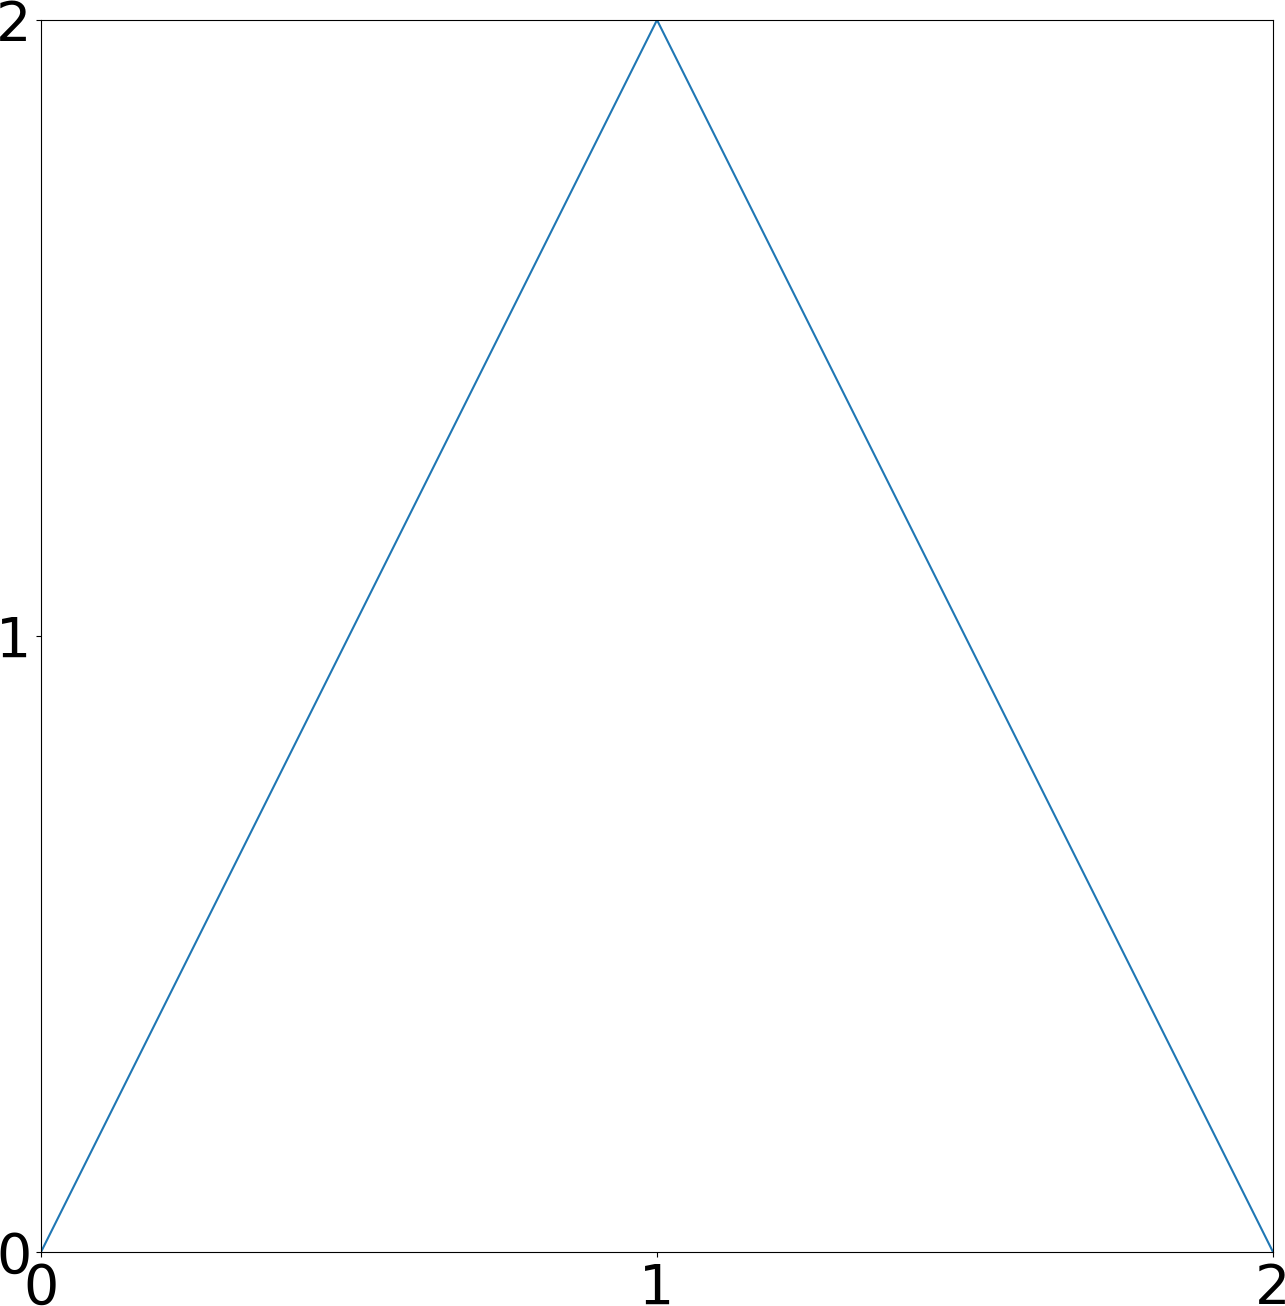
\includegraphics[width=0.48\textwidth]{figure/tent_map.png}
\caption{The tent map $\varphi$.}
\label{fig:tent_map}
\end{figure}

The tent map $\varphi$ is chaotic because a trajectory $x_0,x_1,\ldots$ satisfying
$x_{i+1} = \varphi(x_i)$ exhibits exponential sensitivity to initial condition. An infinitesimal perturbation of absolute value $\delta x$, applied to an initial condition $x_0$, generates a trajectory that is $2 \delta x$ away from $x_1,$ $4 \delta x$ from $x_2$, $8 \delta x$ from $x_3$ and so on. This exponential divergence of two trajectories that start infinitesimally apart is the butterfly effect that characterizes
chaotic dynamics.

It is easy to find periodic solutions for the tent map.
$\frac43$ maps to itself; $\frac45$ and $\frac85$ map to each other;
$\frac47, \frac87$, and $\frac{12}7$ map circularly.  In fact, any rational number evolves into periodic solutions that visit
only a finite set of rational numbers with the same denominator.
This is compatible
with ergodic theory because all rational numbers in $[0,2]$ comprise a subset of Lebesgue measure zero. That is, we would have zero likelihood of getting a
rational number if sampled the Lebesgue measure (the uniform distribution) on $[0,2]$.  Instead, with a 100\% probability, one would get an irrational number
that, when iterated under the tent map, leads to a physical trajectory that distributes uniformly on the interval $[0,2]$.

To understand why a physical solution visits the interval $[0,2]$ at a uniform
frequency, it is helpful to view the tent map from a different perspective.
For a randomly chosen $x_0\in[0,2]$, we can represent it in binary form:
\begin{equation}
    x_0 = \sum_{j=0}^{\infty} \frac{x_{0,j}}{2^j}
\end{equation}
where $x_{0,0}\in\{0,1\}$ is the integer component of $x_0$ and $x_{0,j}\in\{0,1\}$ is the $j$th bit after the binary point.
Let $x_{i+1} = \varphi(x_i)$, then it is straightforward to verify from the definition
of the map that its binary representation
\begin{equation}
    x_i = \sum_{j=0}^{\infty} \frac{x_{i,j}}{2^j}
\end{equation}
would satisfy
\begin{equation} \label{tent_xor}
    x_{i+1,j} = x_{i,0} \veebar x_{i,j+1}
\end{equation}
where $\veebar$ is the xor operator. To see why, note that 
multiplication by 2 is a left-shift operator in binary, and 
subtraction from 4 flips every bit after the binary point. If $x_0$ is chosen uniformly in $[0,2]$, then each bit $x_{0,j},j=0,1,\ldots$ of $x_0$
has equal probability of being 0 or 1, and each bit is independent of other bits.
It follows from Eq. \ref{tent_xor} that each bit $x_{i,j},j=0,1,\ldots$ of $x_i,
i=1,2,\ldots$ has equal probability of being 0 or 1,
and each bit is still independent of the other bits.
Thus, every $x_i$ in this physical solution is uniformly distributed in $[0,2]$.
As the map iterates starting from almost any $x_0$, a physical solution explores the entire interval $[0,2]$ uniformly.

\subsection{Nonphysical solutions Type II: Quasi-physical Solutions}
\label{sec:quasiphysical}
The simplicity of the tent map, as well as its binary form (\ref{tent_xor}),
enables us to study nonphysical solutions that are not periodic.
As in the last section, consider an
\begin{equation}
    x_0 = \sum_{j=0}^{\infty} \frac{x_{0,j}}{2^j}
\end{equation}
in which the bits $x_{0,j}$ are not independent of each other.  Instead,
suppose each bit is more likely to be identical to the previous bit than to be different.
That is, $x_{0,j+1}=x_{0,j}$ with probability $p>\frac12$ for $j=0,1,2,\ldots$.
Then, by Eq. \ref{tent_xor}, the bits of every $x_i, i=1,2,\ldots$ follow the same pattern, namely, each bit repeats the previous bit
with probability $p$. Moreover, consider Eq. \ref{tent_xor} 
for $j=0$ and any $i$:
\begin{equation}
    x_{i+1,0} = x_{i,0} \veebar x_{i,1}
\end{equation}
Because $x_{i,0}=x_{i,1}$ with probability $p>\frac12$, $x_{i+1,0}=0$ with probability 
$p>\frac12$.  Starting from $x_1$, this solution visits $[0,1]$ with
probability $p>\frac12$.  Instead of visiting $[0,1]$ and $[1,2]$ with
equal probability, as a physical solution does, this solution favors $[0,1]$. Since it provably visits the interval $[0,2]$ with a different frequency from that
of a physical solution, this is a nonphysical solution.

If $p = 1$, the bits of $x_0$ are either all zeros or all ones. So, all further iterates when $x_0$ is 0, are 0, and this is a trivial nonphysical solution of type 1. When $x_0$ consists of all ones, the solution eventually becomes 0, and hence is also a nonphysical solution that is eventually periodic (of period 1). Even when this solution does not attain zero in a large number of iterations, it does not 
distribute uniformly on $[0,2]$ like a physical solution 
because all $x_i, i\geq 1$ are of the form $1/2^k$ for some $k \in \mathbb{N}$; other numbers are not visited. Now when $p > \frac12$ but strictly less than 1, 
the solutions we just constructed are both nonphysical and aperiodic.
The bits of $x_0$, though correlated with each other,
still can exhibit an infinite variety of patterns. 
This implies that the solution may not eventually converge to 
any fixed point, nor show any repetitive patterns.  
 As the map iterates, these patterns
shift towards more significant digits, and the solution visits an infinite set of
points. 
 Nevertheless, the solutions observed along a trajectory also 
 do not conform to a uniform distribution on $[0,2]$ since they 
 preferentially visit the first half of this interval.
We call such aperiodic nonphysical solutions ``quasi-physical'' solutions.

\begin{figure}[H]\centering
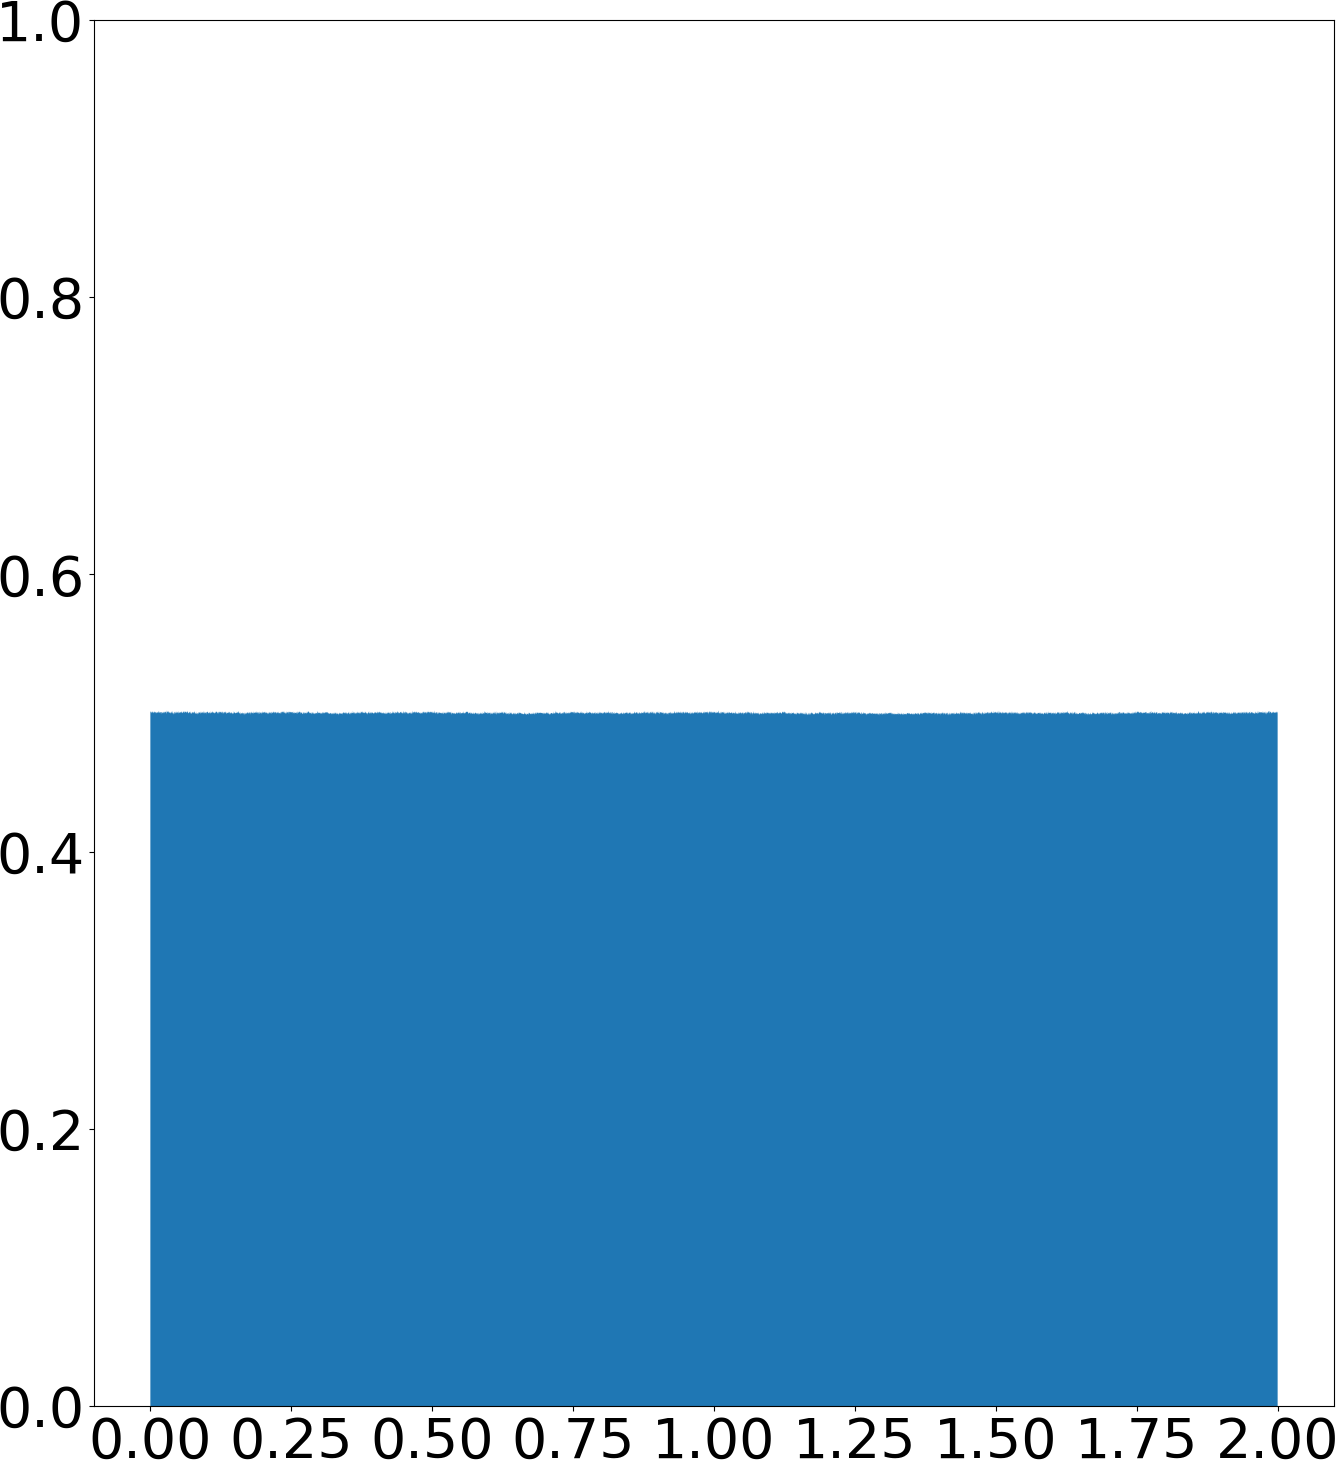
\includegraphics[width=0.48\textwidth]{figure/tent_quasiphysical_hist_p_0.5001.png}
\hspace{0.02\textwidth}
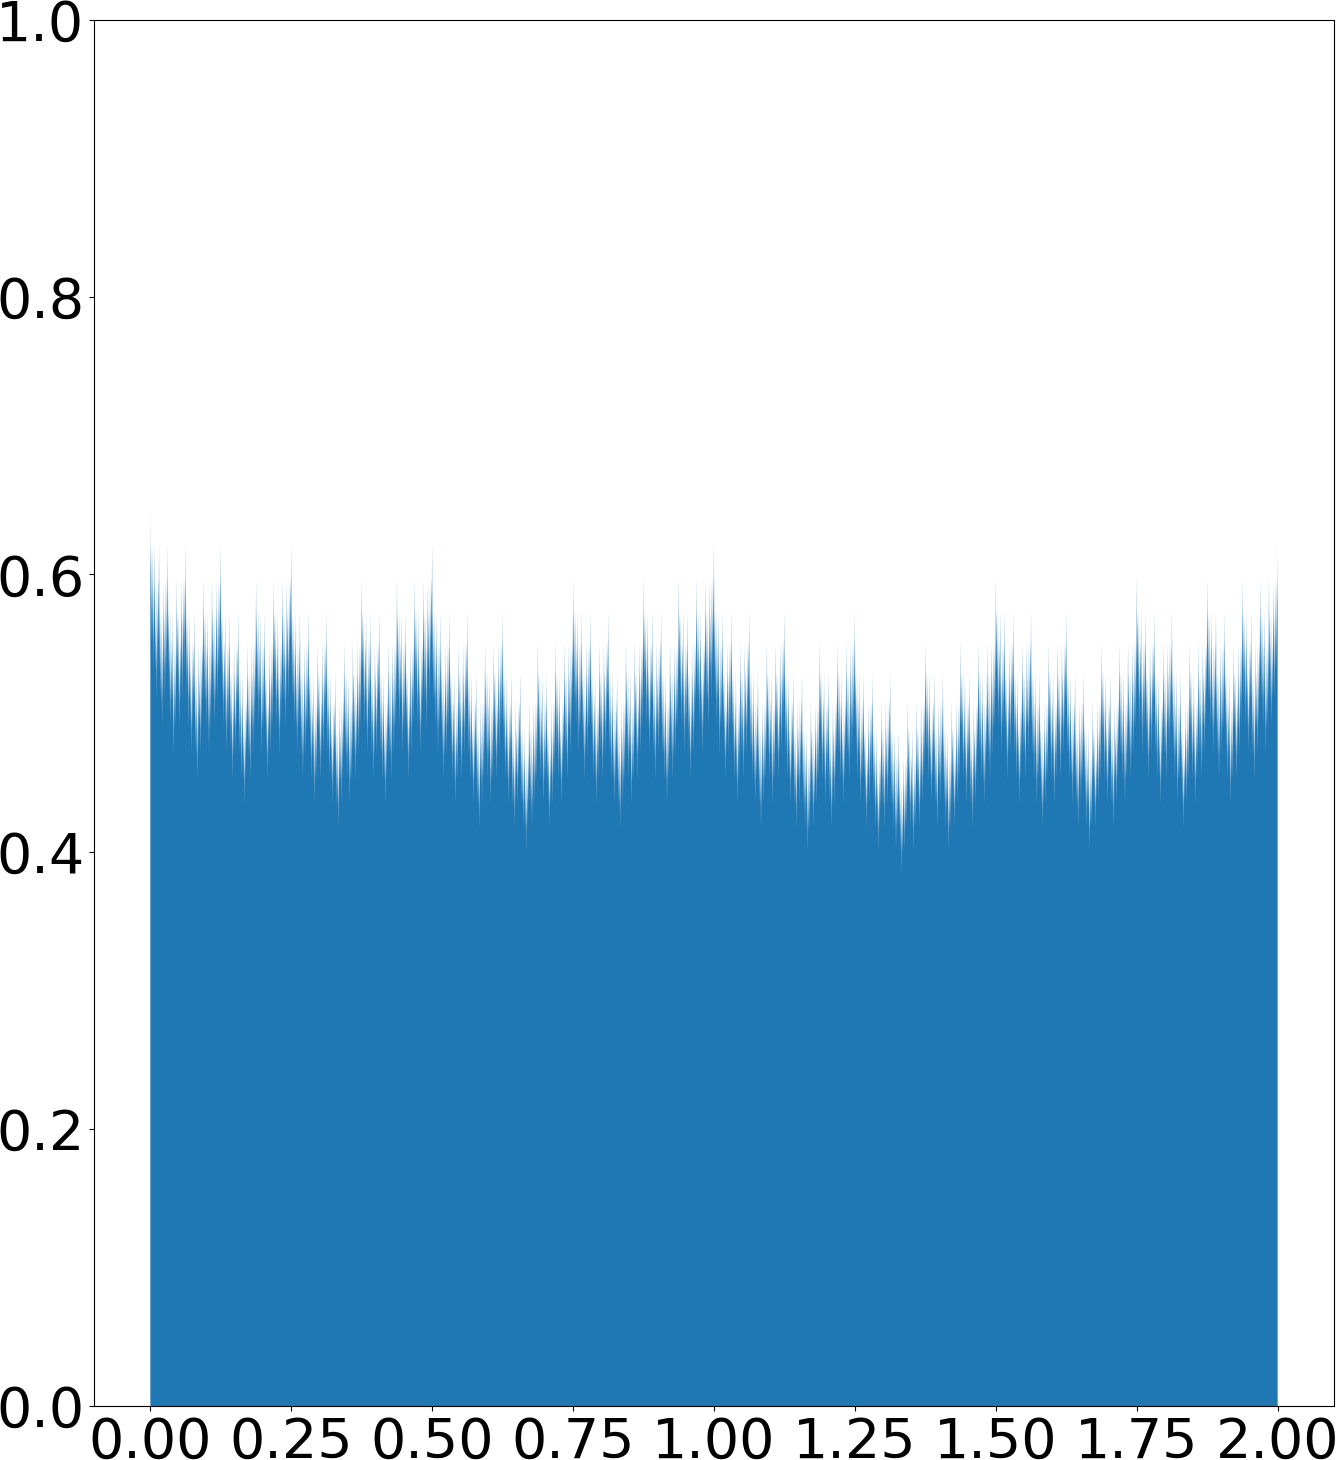
\includegraphics[width=0.48\textwidth]{figure/tent_quasiphysical_hist_p_0.51.png}
\\ \vspace{0.05\textwidth}
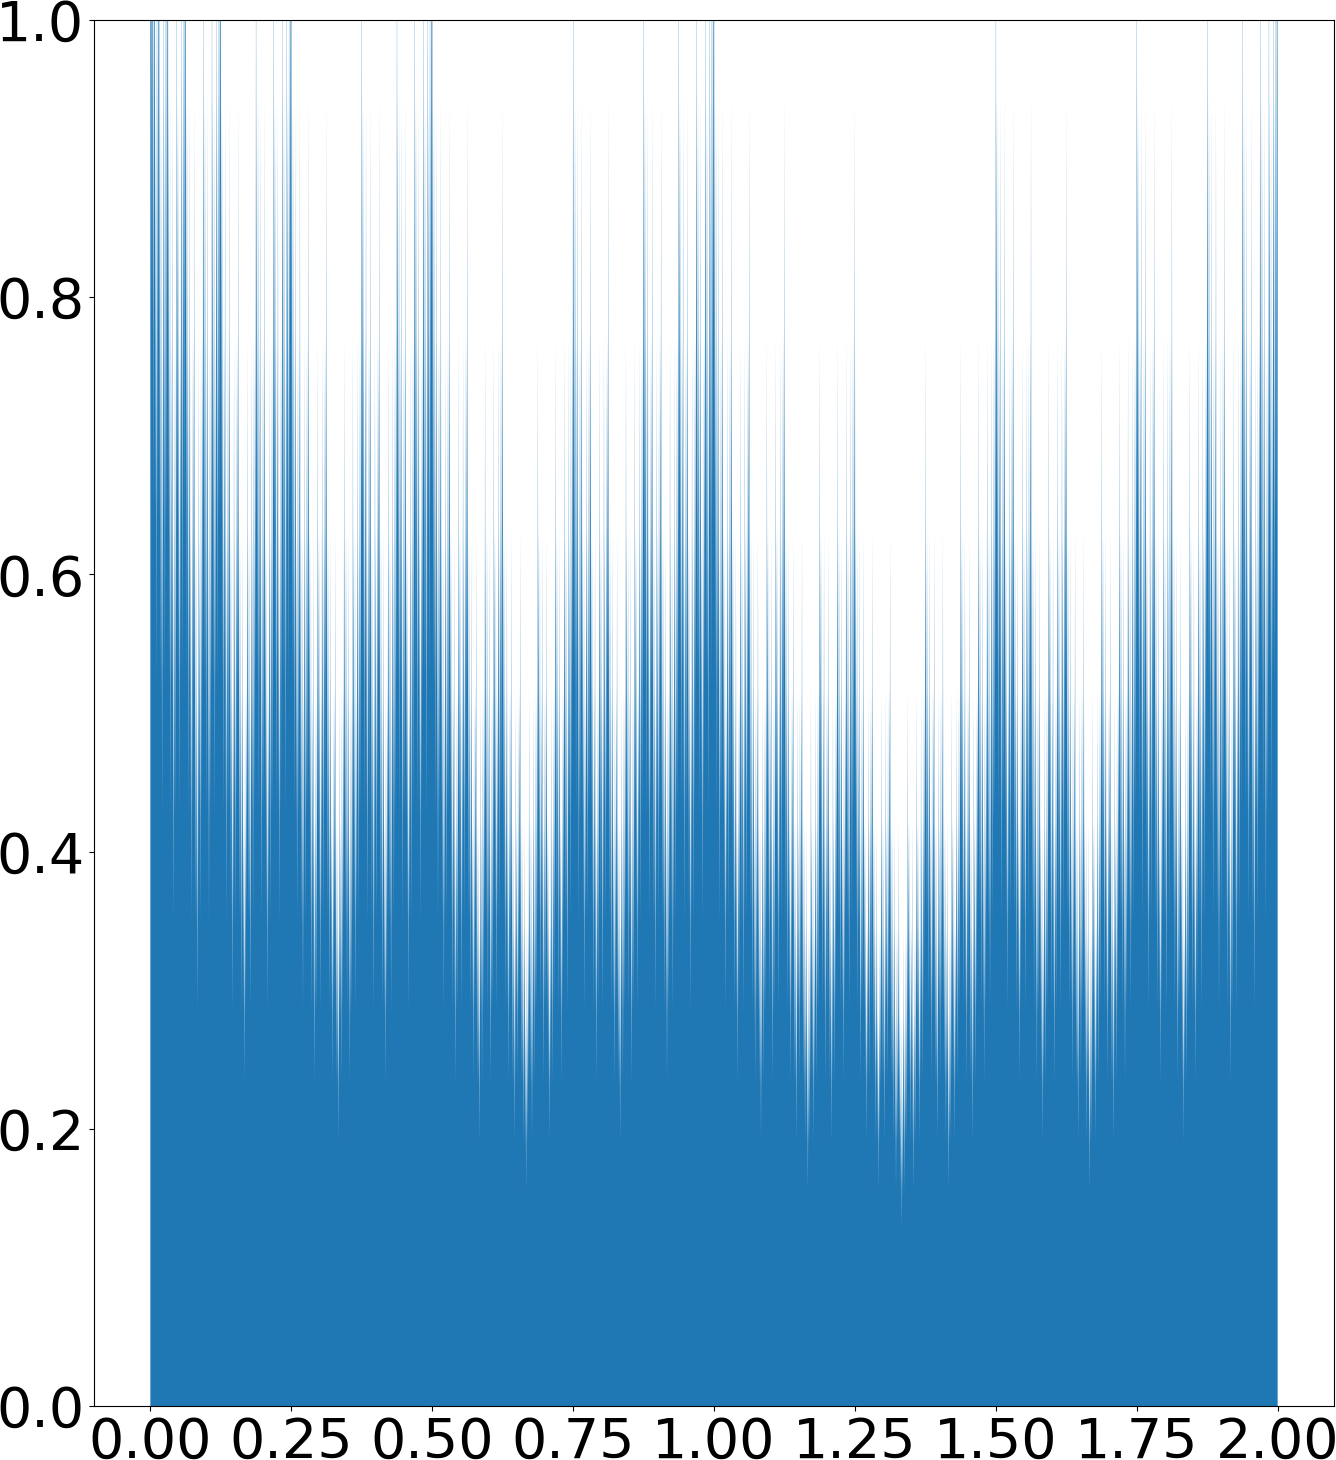
\includegraphics[width=0.48\textwidth]{figure/tent_quasiphysical_hist_p_0.55.png}
\hspace{0.02\textwidth}
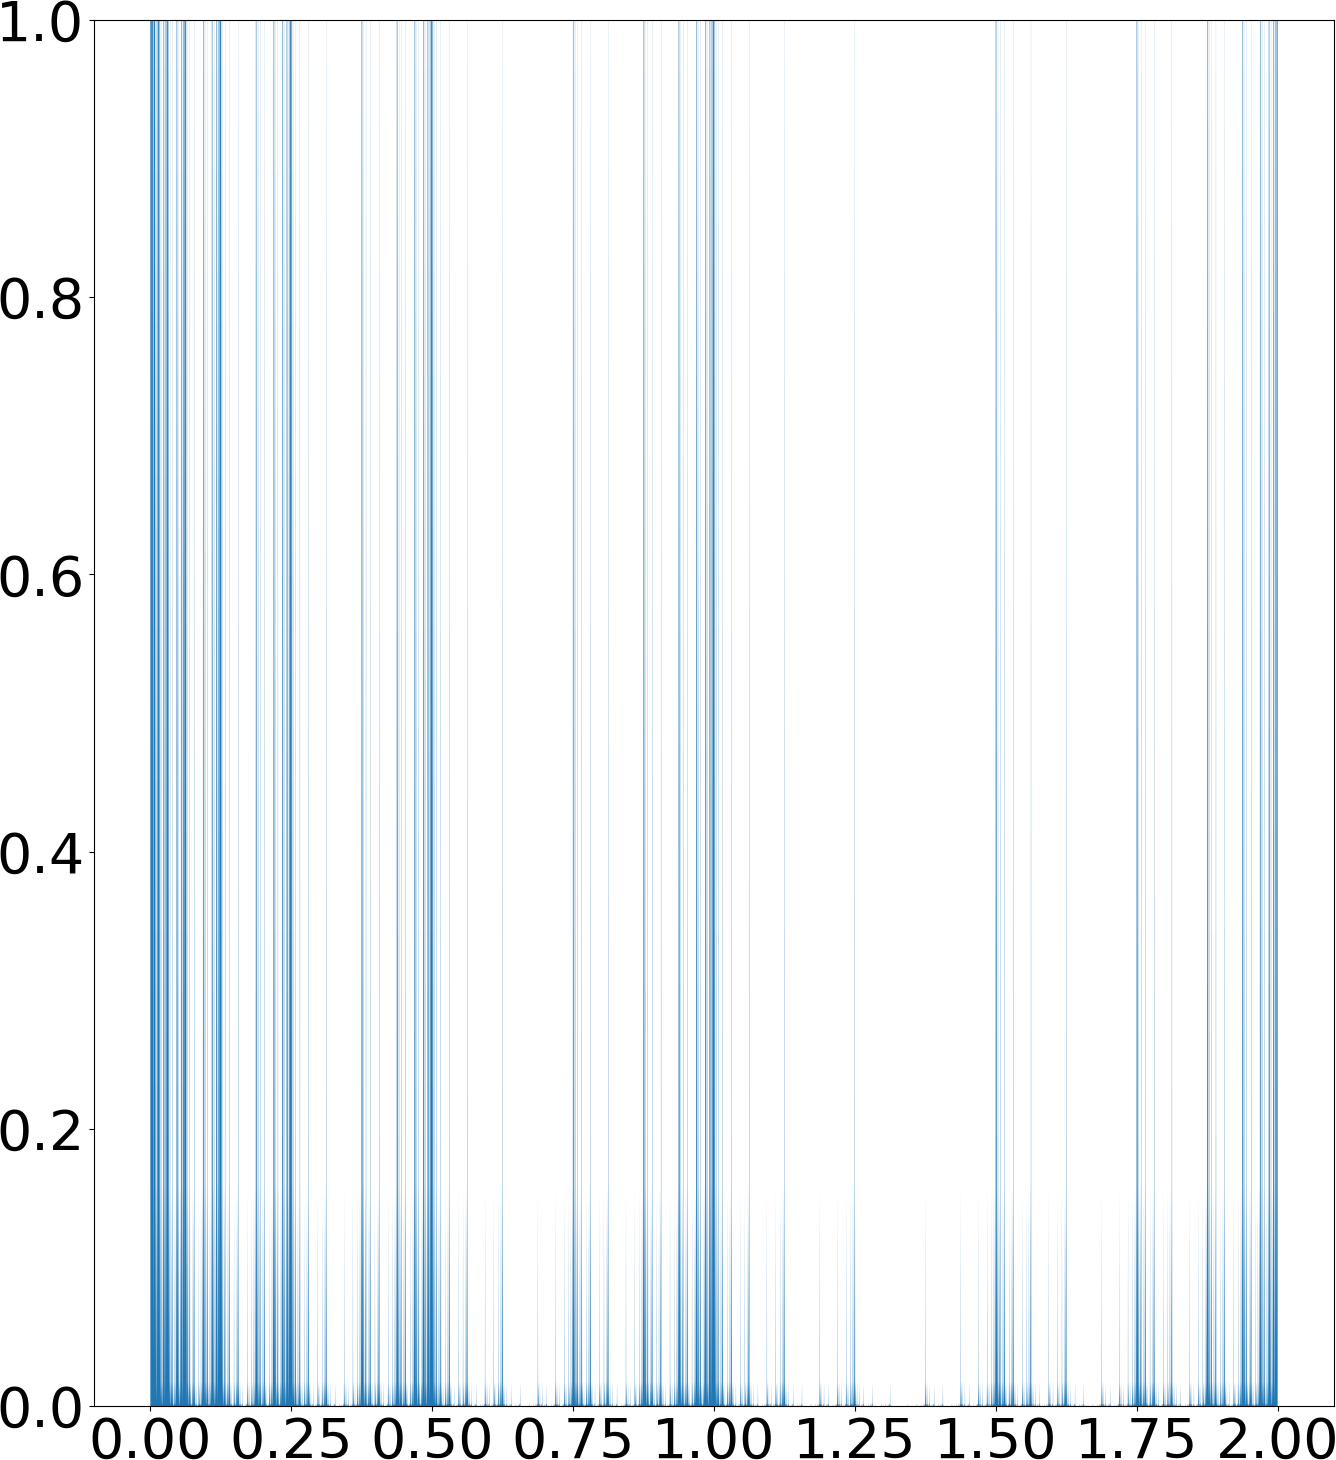
\includegraphics[width=0.48\textwidth]{figure/tent_quasiphysical_hist_p_0.9.png}
\caption{Empirical density function of long solutions (a billion steps)
starting from four points whose binary digits have probability $p$ of
repeating the previous digit.
The solution shown in the top-left plot starts from a point with $p=0.5001$;
top-right: $p=0.51$; bottom-left: $p=0.55$; bottom-right: $p=0.9$.
Note that the empirical densities at larger $p'$s are well above 1.}
\label{fig:tent_quasiphysical}
\end{figure}

Figure \ref{fig:tent_quasiphysical} shows the empirical density functions of
four such quasi-physical solutions.  When $p=0.5001$,
the statistical distribution of the quasi-physical solution
is approximately uniform.  Recall that a physical solution explores $[0,2]$
uniformly.  In this case, the quasi-physical solution has very similar
statistical behavior as a physical solution.  When $p=0.51$, the empirical
distribution becomes ``hairy''.  An apparently fractal pattern emerges.
This fractal pattern further amplifies when $p=0.55$.  Meanwhile,
the density on the left side, $[0,1]$, becomes obviously higher than
the density on the right side, $[1,2]$.  This is consistent with our
theoretical analysis at the beginning of this subsection.
When $p=0.9$, the fractal pattern is so intensified that most
of the solution seem to concentrate in a collection of tiny intervals.
These plots expose the diversity of quasi-physical solutions.
Their statistical distribution can be either
very similar or completely different from that of physical solutions.

So far we have constructed one class of quasi-physical solutions.
It is noteworthy that there are infinite ways to 
construct quasi-physical solutions.  In the binary representation 
of the initial condition $x_0$, any statistical
deviation from equal probability of 0 or 1, or any statistical
dependence among digits would lead to quasi-physical solutions.
One could, for example, construct an $x_0$ in which a bit is
more likely to be 1 than 0 only if it follows two consecutive 0's.
Such $x_0$ would lead to a nonphysical solution.  Its statistical
distribution would differ from any of the plots in Figure
\ref{fig:tent_quasiphysical}.  Nevertheless, as can be
observed in Figure \ref{fig:tent_alternative}, it shows
a remarkable resemblance in its ``hairiness''; some kind of fractal
pattern emerges from the distribution.  A fractal distribution
appears to be a hallmark of quasi-physical solutions.
\begin{figure}[H]\centering
    \centering
    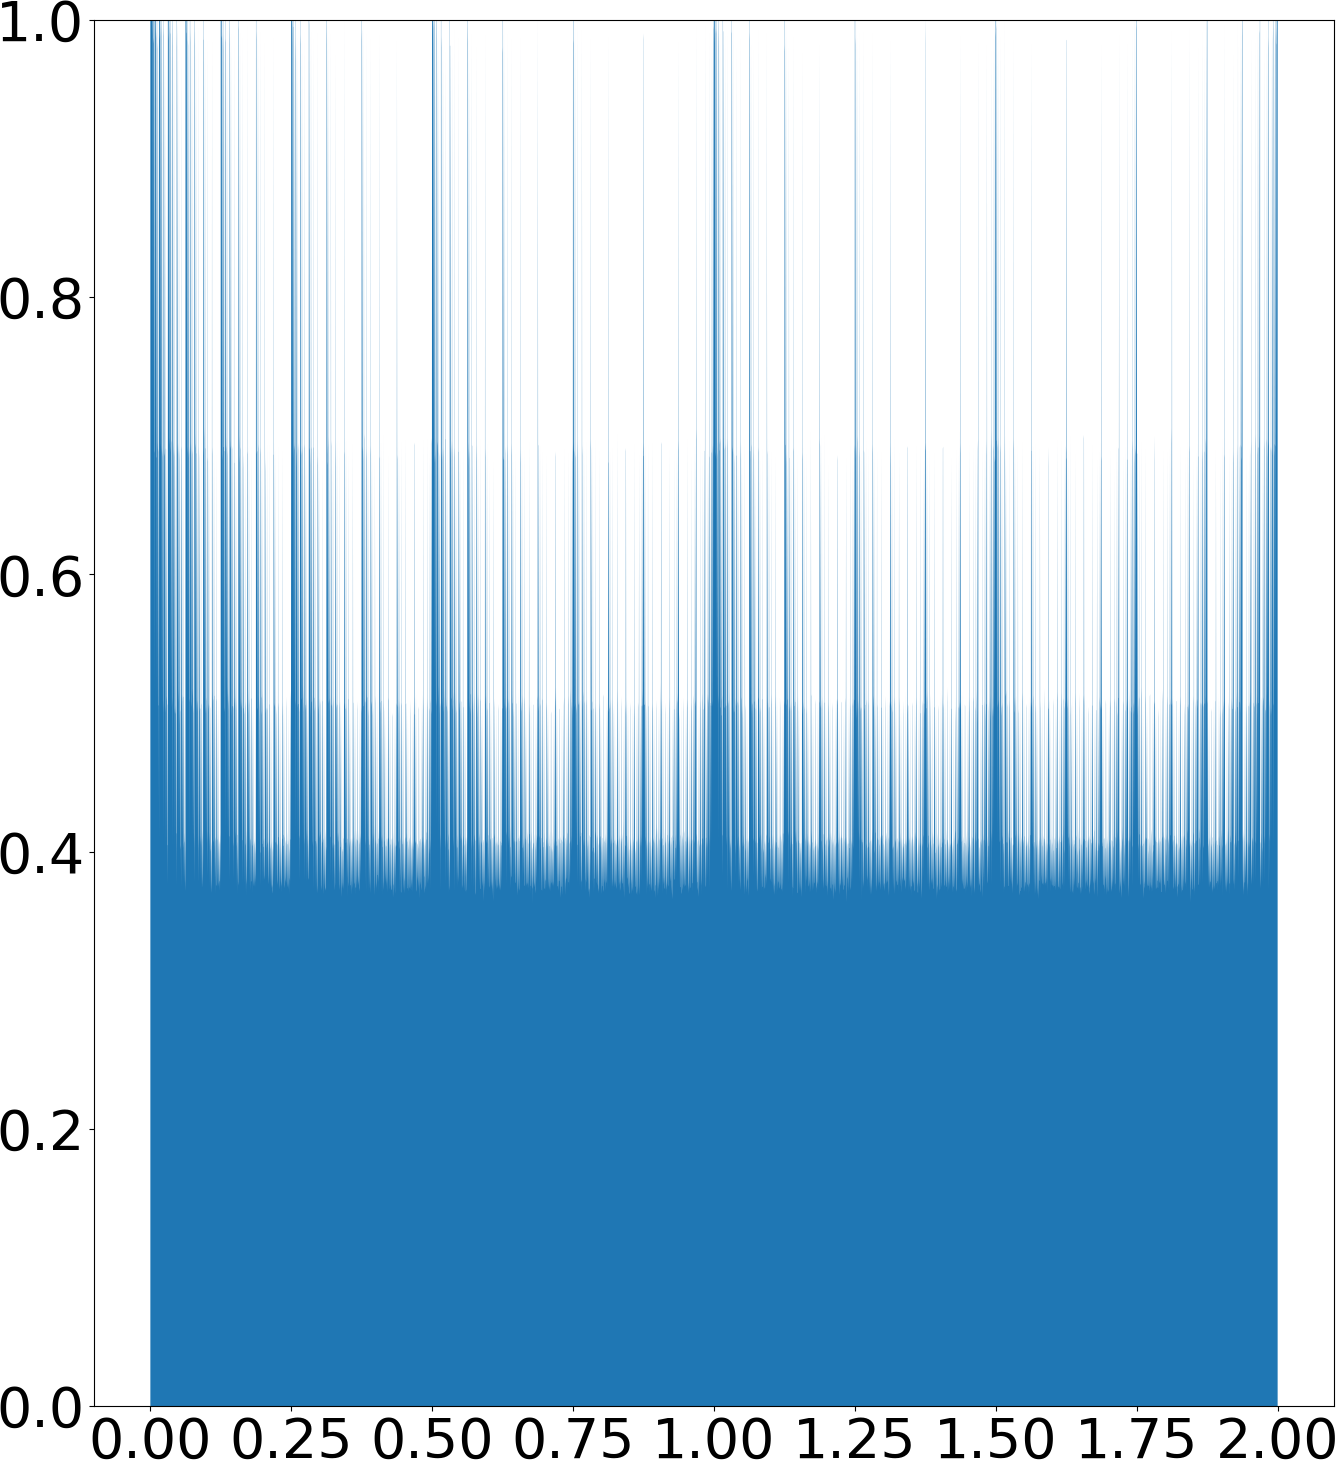
\includegraphics[width=0.48\textwidth]{figure/tent_quasiphysical_alternaive1_hist_p_0.6.png}
    \hspace{0.02\textwidth}
    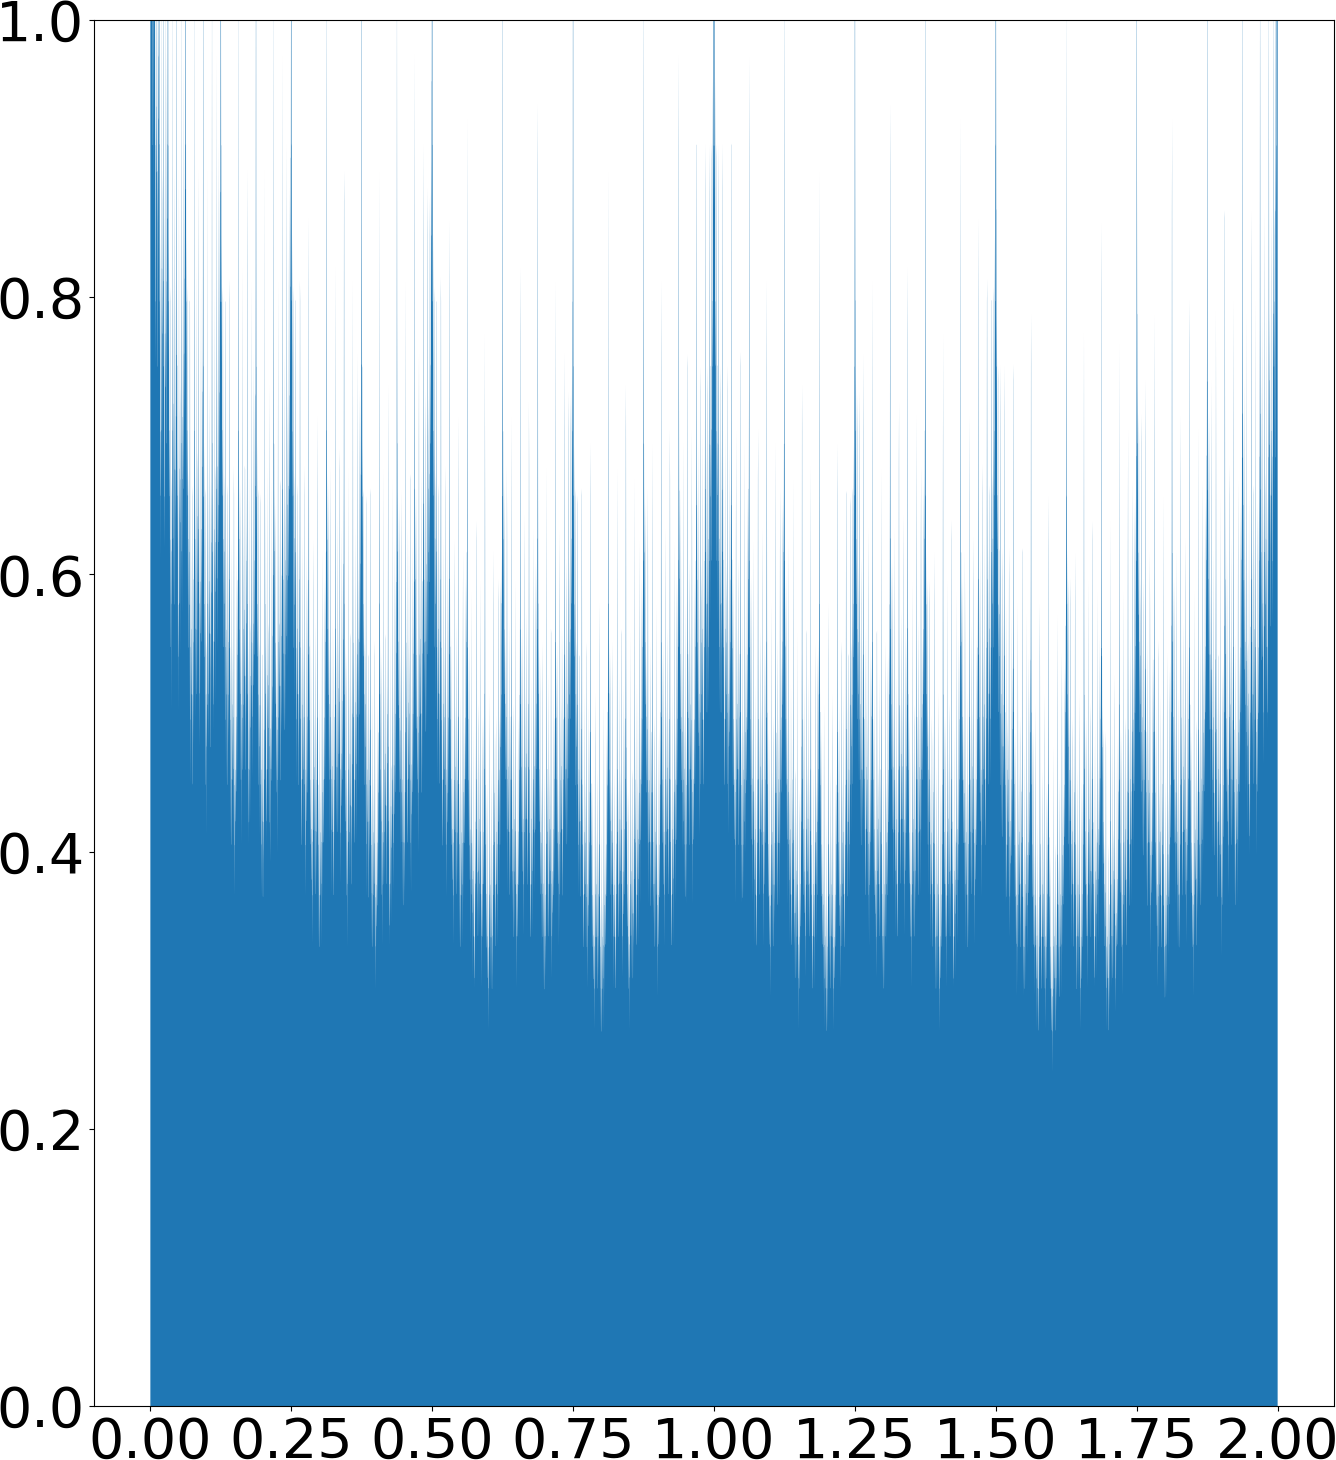
\includegraphics[width=0.48\textwidth]{figure/tent_quasiphysical_alternaive2_hist_p_0.6.png}
    \caption{Empirical distribution function of other quasi-physical solutions.
    The solution shown in the left plot starts from an initial condition
    whose bits are independent and have probability 0.6 of being 0.
    The solution shown in the right plot starts from an initial condition
    whose bits have a probability of 0.6 of being 1 only following two
    consecutive 1's; otherwise a bit is 0 or 1 with equal probability.}
    \label{fig:tent_alternative}
\end{figure}

We have only seen quasi-physical solutions for the tent map.
It is difficult to analytically construct quasi-physical solutions
to the Lorenz equation and other, more complex, governing
equations which typically produce chaotic solutions.  Neverthless, the similarity 
between the tent map and the Lorenz map \cite{tent2}, shown in Figure \ref{fig:lorenz_map}, suggests that
quasi-physical solutions may exist for the Lorenz map, and by
extension, the Lorenz equation.  It is then natural to conjecture
that such aperiodic, non-physical, quasi-physical solutions
exist in general for chaotic dynamical systems.

These quasi-physical solutions raise doubts over the usefulness of shadowing
in some applications.  For example, even if a numerical
solution is shadowed by a solution to the true governing physics,
is the shadowing solution physical or quasi-physical? At first glance, this may 
seem to be a nonissue because almost all solutions are physical. 
It seems reasonable to argue that because the set of
all nonphysical solutions is Lebesgue measure-zero, the probability of finding
a nonphysical solution through shadowing is zero percent.  Such an argument,
as we show in the next section, is wrong.  The probability of
finding a nonphysical solution through shadowing can be, instead of
zero percent, one hundred percent.

\section{Are shadowing solutions physical?}

\subsection{Example of a shadowing solution for the tent map}
\label{sec:sub:shadow-example}
To illustrate the concept of shadowing, consider the tent map, defined
in Eq. \ref{tentmap}, and a scaled version of the map, defined by
\begin{equation} \label{tent_scaled}
    \hat\varphi_s(x) := \begin{cases}
    2x \quad & x < 1+s \\
    4(1+s) - 2x \quad & x \ge 1+s
    \end{cases}
\end{equation}
where $s<<1$.  Note that a small change in $s$ can lead to drastic differences 
between solutions starting from the same initial condition.
As demonstrated in Figure \ref{fig:tent_ivp}, this sensitivity to small
perturbations reflects the chaotic nature of the governing equation.

\begin{figure}[H]   \centering
    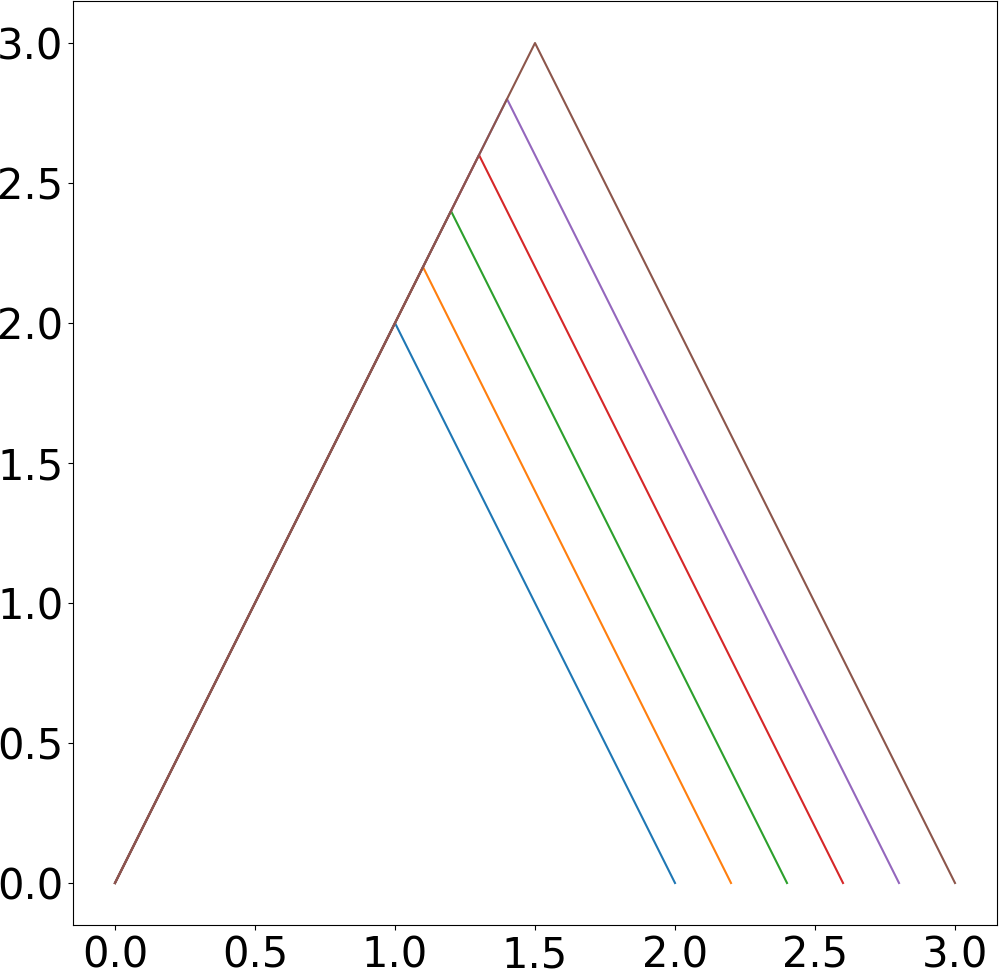
\includegraphics[width=0.48\textwidth]{figure/scaled_tent_map.png}
    \hspace{0.02\textwidth}
    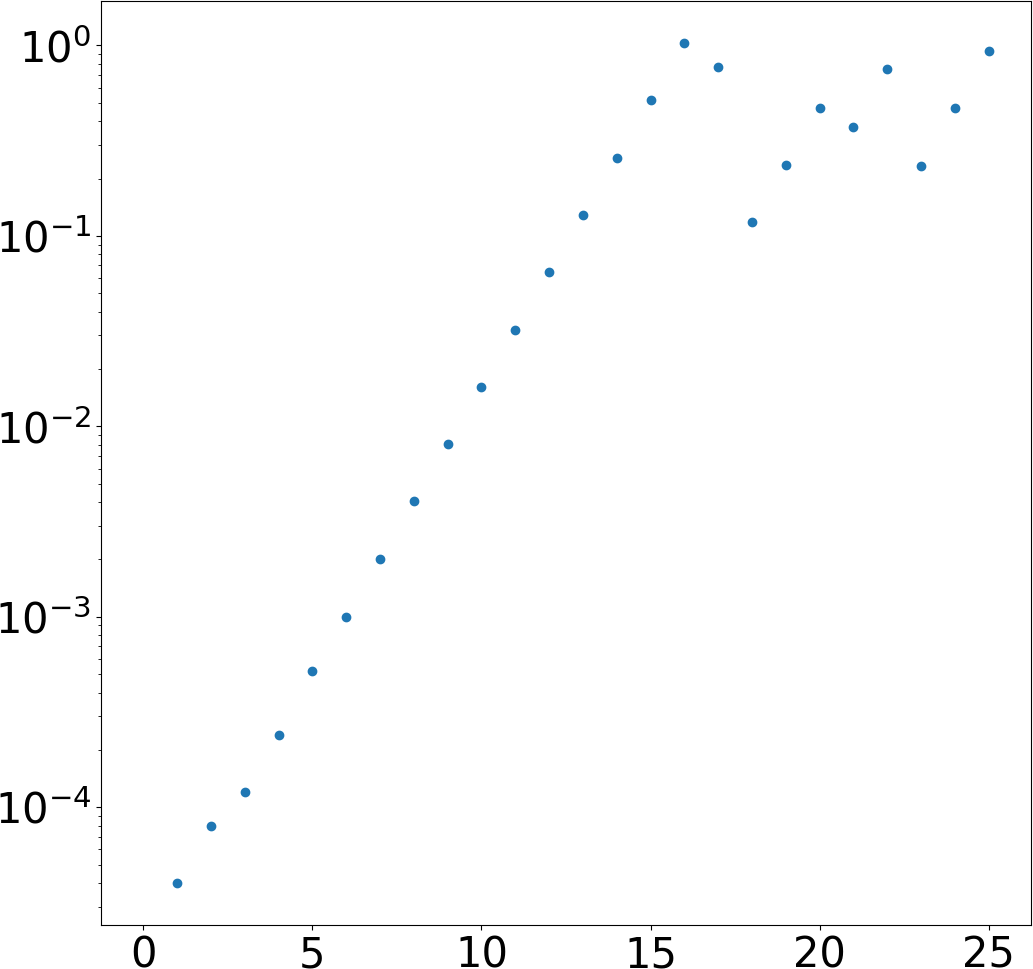
\includegraphics[width=0.48\textwidth]{figure/tent_ivp.png}
    \caption{L: The scaled tent map $\hat{\varphi}_s$ at different values of $s$ between 0 and 1. R: sensitivity to small perturbation in the governing
    equation.
    The y-axis shows the absolute value of the difference between
    two solutions, one satisfying Eq. \ref{tent_scaled},
    one for $s=0$ and the other for $s=10^{-5}$.
    The x-axis shows the iteration number.  The initial condition
    is at $x_0=\pi/2$.
    }
    \label{fig:tent_ivp}
\end{figure}

We can avoid this sensitivity to the governing equation using a coordinated perturbation to the initial condition.
Consider two solutions satisfying Eq. \ref{tent_scaled} at different values of $s$.  Instead of starting from the same
initial condition, these two solutions start from $x_0 (1 + s)$ with
the same $x_0$ but their respective values of $s$.  It can be shown that
the solution of these two equations would be
$x_i (1+s), i=0,1,\ldots$ with their respective values of $s$,
where $x_{i+1}=\varphi(x_i)$ satisfies the original
tent map (Eq. \ref{tentmap}).  When the values of $s$ are similar between
the two solutions, this pair of solutions stays uniformly close to each
other forever.  Such a true solution of the governing equation
that stays close to a given perturbed solution over a long time, is known as a \emph{shadowing} solution. In this example, the perturbed solution satisfies a 
slightly different governing equation.

For every solution $\hat{x}_i,i=0,\ldots$ satisfying Eq. \ref{tent_scaled}, there is a shadowing solution satisfying Eq. \ref{tentmap}: $x_i:= \hat{x}_i/(1+s)$.  The map,
\begin{equation} \label{conjugate_scaled}
    \hat{h}_s(x):=x/(1+s)
\end{equation}
is known as a \emph{conjugacy} between the two maps $\varphi$ and $\hat{\varphi_s}$ 
because it satisfies
\begin{equation} \label{conjugate_def}
    \varphi(\hat{h}_s(x)) = \hat{h}_s(\hat\varphi_s(x))\;,\quad \forall\: x
\end{equation}
or equivalently, $\varphi\circ h_s \equiv h_s\circ\hat\varphi_s$.
Such conjugacy maps can generally help us construct shadowing solutions.
For every solution satisfying
$\hat{\varphi}_s$, $h_s$ maps it to a shadowing solution satisfying $\varphi$.

Is the shadowing solution a physical solution?  In this example,
the answer is almost surely positive.  We can demonstrate that
almost any solution of the scaled tent map (Eq. \ref{tent_scaled}) is uniformly
distributed in $[0, 2(1+s)]$ -- we can repeat our analysis
in Section \ref{sec:tent} but represent our initial condition as
$x_0= (1+s) \sum_{j=0}^\infty x_{0,j} / 2^j$.  Its shadowing solution,
which satisfies the original tent map (Eq. \ref{tentmap}), can be obtained through the
conjugacy (Eq. \ref{conjugate_scaled}).  Thus, the distribution
of the shadowing solution can be obtained by mapping a uniform
distribution in $[0,2(1+s)]$ through the conjugacy map.
This leads to a uniformly distribution in $[0,2]$, which is
precisely the distribution of a physical solution of the tent map.

This simple example is useful in illustrating the concept of shadowing
and the utility of the conjugacy map.  But it is rather special
in that the shadowing solution is almost always physical.  Our next
example introduces a tilted version of the tent map.  Although
the tilting perturbation to the tent map seems as simple as the
scaling perturbation, the shadowing solution, as we will see,
is almost always a quasi-physical solution.

\subsection{An example of quasi-physical shadowing solution}
\label{sec:sub:quasi-physical-shadow}
The tilted tent map is defined as
\begin{equation} \label{tent_tilted}
    \tilde\varphi_s(x) := \begin{cases}
    \frac2{1+s} x \quad & x < 1+s \\
    \frac2{1-s}(2-x) \quad & x \ge 1+s
    \end{cases}
\end{equation}
When $s=0$, this map is identical to the tent map (Eq. \ref{tentmap}).
Let $\tilde{x}_{i+1}=\tilde\varphi_s(\tilde{x}_i), i=0,1,\ldots$ be a solution of 
$\tilde{\varphi}_s$ that is also a perturbed solution of $\varphi$.
As we explained in the previous subsection,
the corresponding 
shadowing solution, which solves $\varphi$, can be found through a conjugacy map $\tilde{h}_s$ that connects the solutions of $\varphi$ and $\tilde{\varphi}_s$.
If $\varphi\circ \tilde{h}_s \equiv \tilde{h}_s\circ\tilde\varphi_s$,
then $x_i=\tilde{h}_s(\tilde{x}_i), i=0,1,\ldots$ is the shadowing solution 
that satisfies $x_{i+1} = \varphi(x_i)$, corresponding to the perturbed solution 
$\tilde{x}_i,i=0,1,\cdots$.

The conjugacy map, although more complex than the one
in the last subsection, has the following closed form:
\begin{equation} \label{conjugate_tilted}
    \tilde{h}_s(x) = \sum_{j=0}^{\infty} \frac{\xi_{s,j}(x)}{2^j}\;,
\end{equation}
where
\begin{equation} \label{conjugate_tilted_helper}
    \xi_{s,j}(x) := \begin{cases}
    0 & j=0, x<1+s \\
    1 & j=0, x\ge 1+s \\
    \xi_{s,j-1}(x) & j>0, \tilde\varphi_s^j(x) < 1+s \\
    1 - \xi_{s,j-1}(x) & j>0, \tilde\varphi_s^j(x) \ge 1+s.
    \end{cases}
\end{equation}
In the above expression, $\tilde{\varphi}^j_s$ refers to the $j$-time 
composition of $\tilde{\varphi}_s.$ That is, if $\tilde{x}_{j+1} = \tilde{\varphi}_s(\tilde{x}_j), j = 0,1,\cdots,$ is a solution, $\tilde{\varphi}_s^i(\tilde{x}_j) = \tilde{x}_{j+i},\quad i,j = 0,1,\cdots$. 
To see why $\tilde{h}_s$ constructed in Eq. \ref{conjugate_tilted} satisfies the definition of a conjugacy map --
$\tilde{h}_s(\tilde\varphi_s(x)) = \varphi(\tilde{h}_s(x))$ for all $x$ --
we need to analyze two cases: $x<1+s$ and $x\ge 1+s$.
\begin{figure}[H]
  \centering
    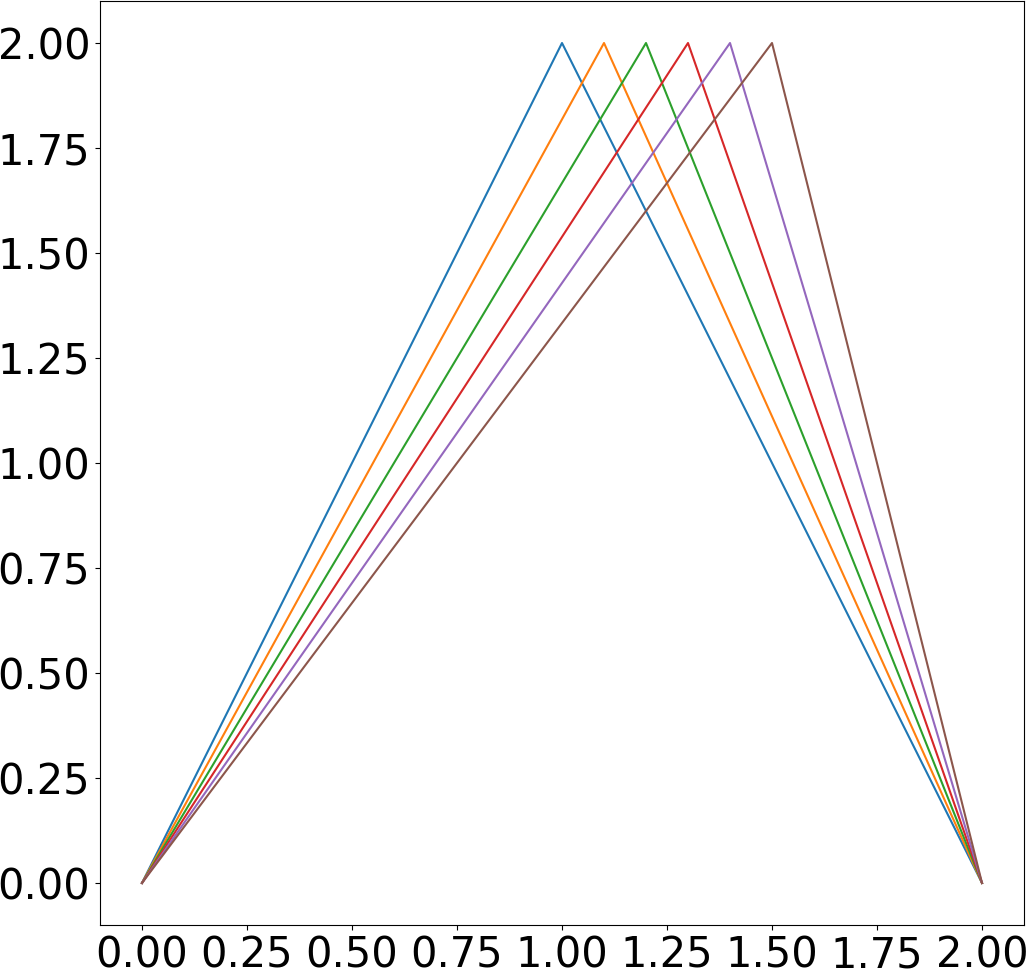
\includegraphics[width=0.48\textwidth]{figure/tilted_tent_map.png}
    \hspace{0.02\textwidth}
    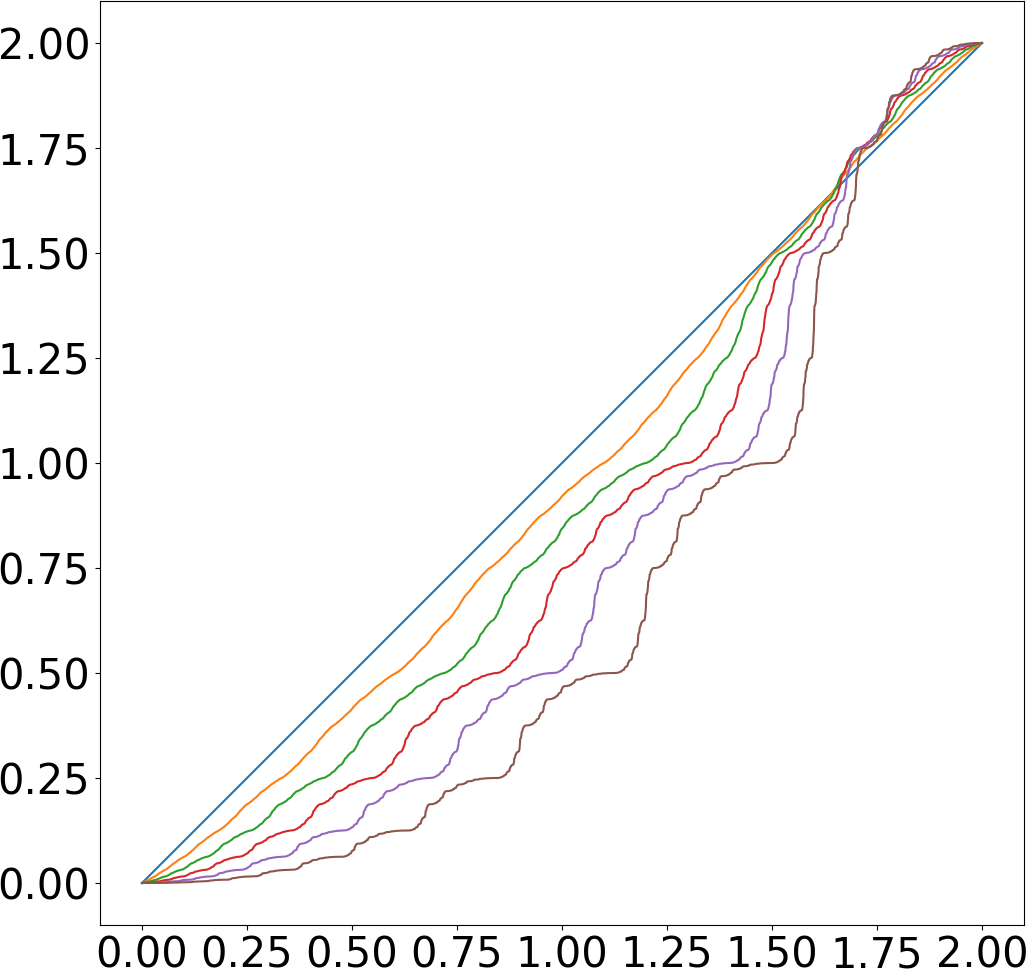
\includegraphics[width=0.48\textwidth]{figure/tilted_conjugate_map.png}
    \\ \vspace{0.02\textwidth}
     \caption{L: the tilted tent map Eq. \ref{tent_tilted} for $s=0, 0.1, 0.2, 0.3, 0.4,$ and 0.5. R: the conjugacy $\tilde{h}_s$ between the tent map (Eq. \ref{tentmap})
    and the tilted tent map (Eq. \ref{tent_tilted}), evaluated using
    Eq. \ref{conjugate_tilted}-\ref{conjugate_tilted_helper}, for the same set of $s$ as the
    left plot.}
     \label{fig:tilted_tent_conjugate}
\end{figure}
When $x<1+s$, $\xi_{s,0}(x)=0$; thus
$\tilde{h}_s(x) = \sum_{j=1}^{\infty} \frac{\xi_{s,j}(x)}{2^j}$.
Inside this infinite series, $\xi_{s,1}(x)=\xi_{s,0}(x)=0$ if $\tilde\varphi_s(x)<1+s$,
or $\xi_{s,1}(x)=1-\xi_{s,0}(x)=1$ if $\tilde\varphi_s(x)\ge 1+s$.
Thus, $\xi_{s,1}(x) = \xi_{s,0}(\tilde{\varphi}_s(x))$ according to the definition of $\xi_{s,0}$.
Using this as the base case, one can inductively verify that
$\xi_{s,j+1}(x) = \xi_{s,j}(\tilde\varphi_s(x))$
for all $j>0$, using just the definitions of $\xi_{s,j}$ and $\xi_{s,j+1}$.
Therefore,
$\tilde{h}_s(x) = \frac12 \sum_{j=0}^{\infty} \frac{\xi_{s,j}(\tilde\varphi_s(x))}{2^j}
=\frac12 \tilde{h}_s(\tilde\varphi_s(x))$.
On the other hand, because
$\tilde{h}_s(x) = \sum_{j=1}^{\infty} \frac{\xi_{s,j}(x)}{2^j}\le1$,
$\varphi(\tilde{h}_s(x)) = 2\tilde{h}_s(x)$ according
to the definition of $\varphi$.  Thus,
$\varphi(\tilde{h}_s(x)) = \tilde{h}_s(\tilde\varphi_s(x))$ holds when $x<1+s$.

When $x\ge1+s$, $\xi_{s,0}(x)=1$; thus
$\tilde{h}_s(x) = 1+ \sum_{j=1}^{\infty} \frac{\xi_{s,j}(x)}{2^j}
                = 2- \sum_{j=1}^{\infty} \frac{1-\xi_{s,j}(x)}{2^j}$.
Inside this infinite series, $1-\xi_{s,1}(x)=1-\xi_{s,0}(x)=0$ if $\tilde\varphi_s(x)<1+s$,
or $1-\xi_{s,1}(x)=\xi_{s,0}(x)=1$ if $\tilde\varphi_s(x)\ge 1+s$.
Thus, $1-\xi_{s,1}(x) = \xi_{s,0}(\tilde{\varphi}_s(x))$ according to the definition of $\xi_{s,0}$.
Using this as the base case, one can inductively verify that
$1-\xi_{s,j+1}(x) = \xi_{s,j}(\tilde\varphi_s(x))$
for all $j>0$, using just the definitions of $\xi_{s,j}$ and $\xi_{s,j+1}$.
Therefore,
$\tilde{h}_s(x) = 2 - \frac12 \sum_{j=0}^{\infty} \frac{\xi_{s,j}(\tilde\varphi_s(x))}{2^j}
=2 - \frac12 \tilde{h}_s(\tilde\varphi_s(x))$.
On the other hand, because
$\tilde{h}_s(x) = 1+\sum_{j=1}^{\infty} \frac{\xi_{s,j}(x)}{2^j}\ge 1$,
$\varphi(\tilde{h}_s(x)) = 4 - 2 \tilde{h}_s(x)$ according
to the definition of $\varphi$.  Thus,
$\varphi(\tilde{h}_s(x)) = \tilde{h}_s(\tilde\varphi_s(x))$ also holds when $x\ge 1+s$.

\begin{figure}[H]
   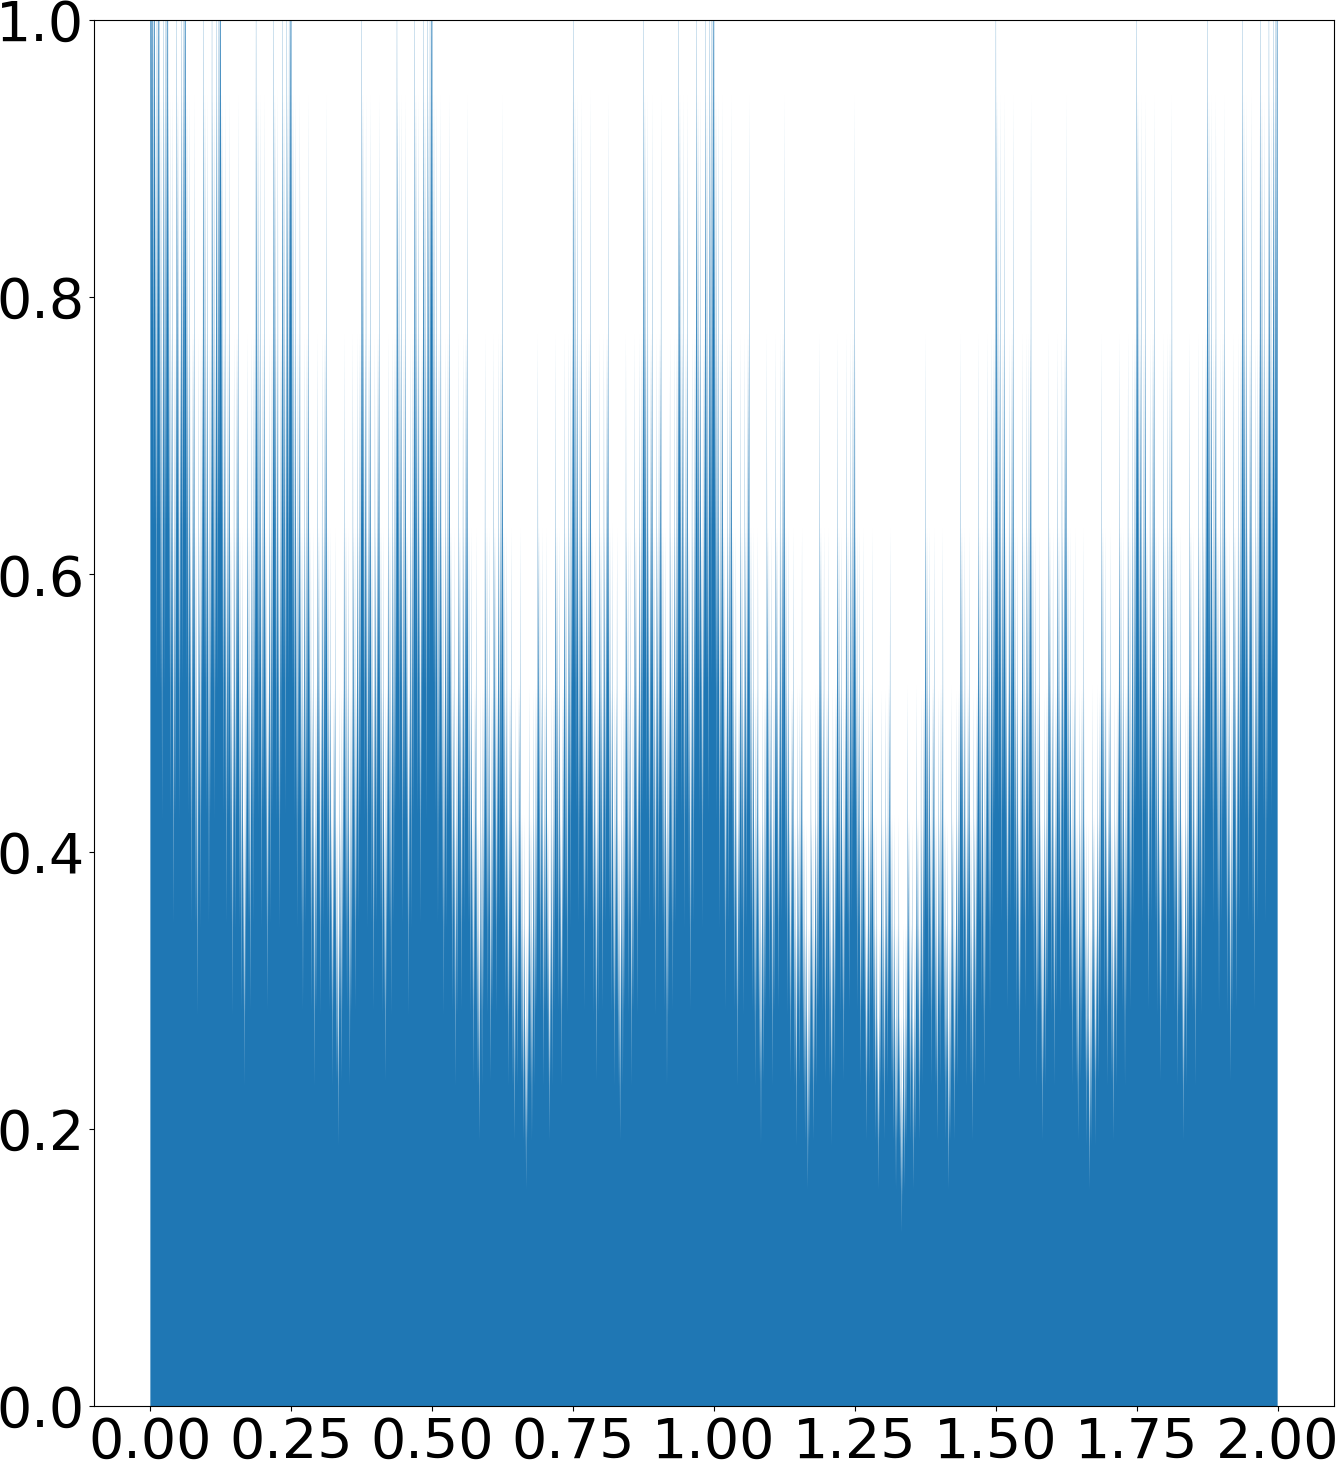
\includegraphics[width=0.48\textwidth]{figure/tilted_conjugate_density_0.1.png}
    \hspace{0.02\textwidth}
    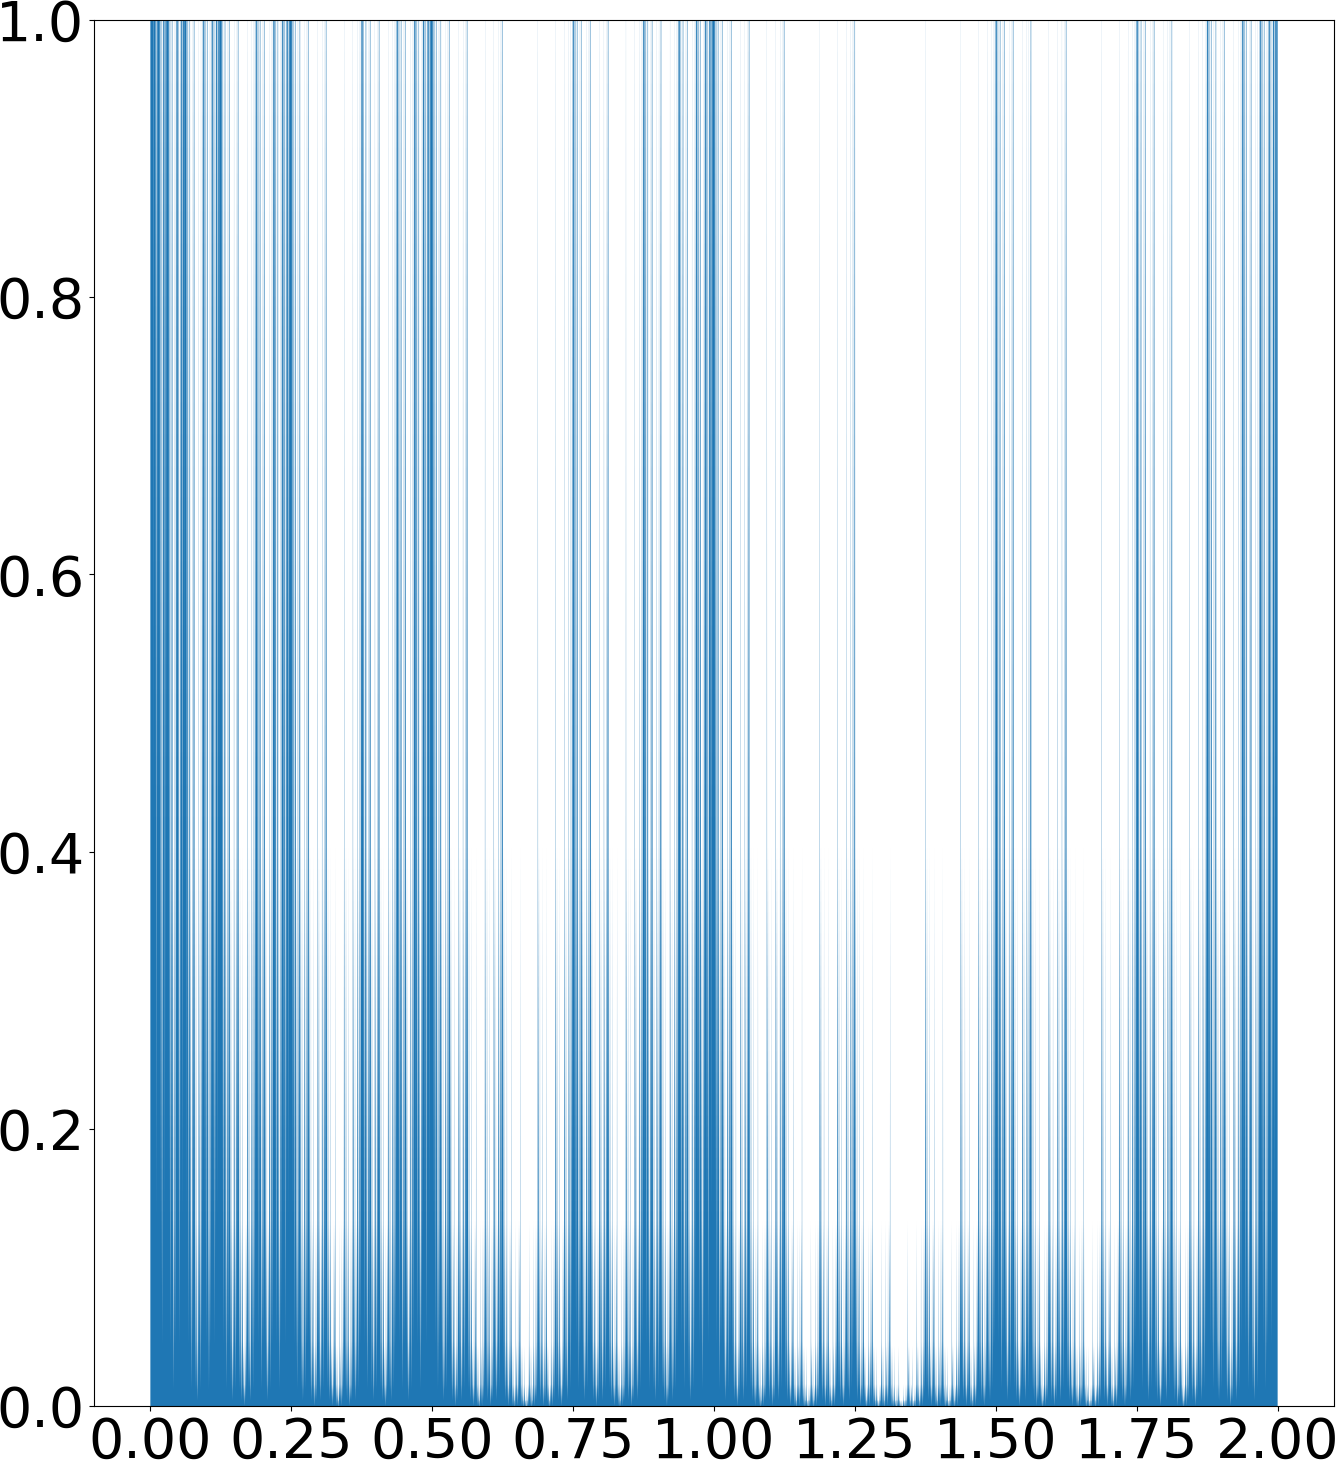
\includegraphics[width=0.48\textwidth]{figure/tilted_conjugate_density_0.5.png}
   \caption{
     L: the density of a trajectory satisfying Eq. \ref{tentmap}
    that shadows a random trajectory satisfying Eq. \ref{tent_tilted} for $s=0.1$.
    R: the density of a trajectory satisfying Eq. \ref{tentmap}
    that shadows a random trajectory satisfying Eq. \ref{tent_tilted} for $s=0.5$.
    }
    \label{fig:tilted_tent_density}
\end{figure}

Figure \ref{fig:tilted_tent_density} shows how fractal the conjugacy map is.
This fractal conjugacy map transforms a uniform distribution in $[0,2]$ into
a fractal distribution similar to the ones plotted in Section \ref{sec:quasiphysical}.
In fact, we will show that the fractal distribution obtained by mapping a uniform
distribution through $\tilde{h}_s$ is exactly the family of distributions
shown in Figure \ref{fig:tent_quasiphysical}.  We will also show that
a physical solution of the tilted tent map (Eq. \ref{tent_tilted}) is uniformly
distributed in $[0,2]$.  Thus, for almost any physical solution of the
tilted tent map, a shadowing solution of the original tent map, obtained
through the conjugate map $\tilde{h}_s$, has a fractal distribution.
Such a shadowing solution is therefore a quasi-physical solution of
the tent map.

We first show that a physical solution of the tilted tent map 
(\ref{tent_tilted}) is uniformly distributed in $[0,2]$, for
any $0\le s<1$.
According to the ergodic theory and the properties of the SRB measure of 
one-dimensional chaotic systems (\cite{young}), 
we only need to show that the uniform
distribution is stationary under the tilted tent map.
The function $\tilde{\varphi}_s$ stretches an infinitesimal
region around each $x$ by the absolute value of the derivative at $x$; 
hence, a uniform density on an infinitesimal region around $\tilde{\varphi}_s(x)$ 
is reduced by the same factor. In other words, let $\tilde{\rho}(x)$ 
be the map of a uniform density on $[0,2]$, through $\tilde{\varphi}_s$. Then, 
$\tilde{\rho}(\tilde{\varphi}_s (x)) = 0.5/|\tilde \varphi_s'(x)| + 0.5/|\tilde \varphi_s'(2-x)|,$ where the two terms express the conservation of probability 
from the two pre-images of $\tilde{\varphi}_s$. Substituting the piecewise constant 
derivative of $\tilde{\varphi}_s$ on the two intervals, $[0,1+s)$ and $[1+s,2]$,
we have $\tilde{\rho}(\tilde{\varphi}_s (x)) = 0.25(1+s) + 0.25(1-s) = 0.5,$ at 
all $x.$ Hence, a uniform density of 0.5 is unaltered by mapping through 
$\tilde\varphi_s(x)$.

We now show that the conjugacy $\tilde{h}_s$ maps a uniform
distribution to a fractal.  Here we use the closed forms Eqs. \ref{conjugate_tilted}-\ref{conjugate_tilted_helper}.
If $x$ is a random number drawn uniformly in $[0,2]$,
it has $\frac{1+s}2$ probability of being less than $1+s$.
Thus, $\xi_{s,0}(x)=0$ with probability $\frac{1+s}2$.
This means, according to Eq. \ref{conjugate_tilted},
$\tilde{h}_s(x)<1$ with probability $\frac{1+s}2$:
$\tilde{h}_s(x)$ is more likely to lie in the left half
of the domain $[0,2]$.
Furthermore, for $j\ge 0$, $\xi_{s,j+1}(x)=\xi_{s,j}(x)$
with probability $\frac{1+s}2$ since each $\tilde{\varphi}^j_s(x)$ is sampled
from the uniform distribution on $[0,2]$.  This probability has direct
implication on $\tilde{h}_s(x)$ since, again by Eq. (\ref{conjugate_tilted}),
$\xi_{s,j}$ is the $j$th bit in the binary representation of $\tilde{h}_s$ --
each bit repeats the previous one with probability
$\frac{1+s}2$.  For a uniformly random
$x$, $\tilde{h}_s(x)$ is exactly the kind of initial condition
we used to construct the quasi-physical solution
in Section \ref{sec:quasiphysical}, with $p=\frac{1+s}2$.
\nisha{This is so well set up and awesome!}
Since this analysis holds for any $x$ sampled uniformly on $[0,2]$, we can conclude that
the shadowing solution is almost surely nonphysical.  Let $x_{s,i},i=0,1,\ldots$ be a solution
to the tilted tent map $\tilde{\varphi}_s$ with $x_{s,0}$ chosen 
randomly in $[0,1+s]$.  Then, with a hundred percent probability,
it is a physical solution that uniformly visits the domain $[0,2]$.
Its shadowing solution $\tilde{h}_s(x_{s,i}),i=0,1,\ldots$, however,
is a quasi-physical solution, also with a hundred percent probability.
It explores $[0,2]$ at a nonuniform frequency with a fractal probability distribution.

\subsection{Are general shadowing solutions physical?}

In the previous subsection, we examined a tilting perturbation to the tent map.
We derived the fractal conjugacy map, and showed that a typical shadowing trajectory
is exactly the quasi-physical solution we analyzed in Section \ref{sec:quasiphysical}.
This example contrasts with Section \ref{sec:sub:shadow-example}, in which the
shadowing solutions of a different perturbation, the scaling perturbation,
are physical solutions.  Which situation is more typical?  When we make other
types of perturbations, do we expect to observe physical or nonphysical
shadowing solutions?


%%
%%\begin{figure}[H]
%%    \centering
%%    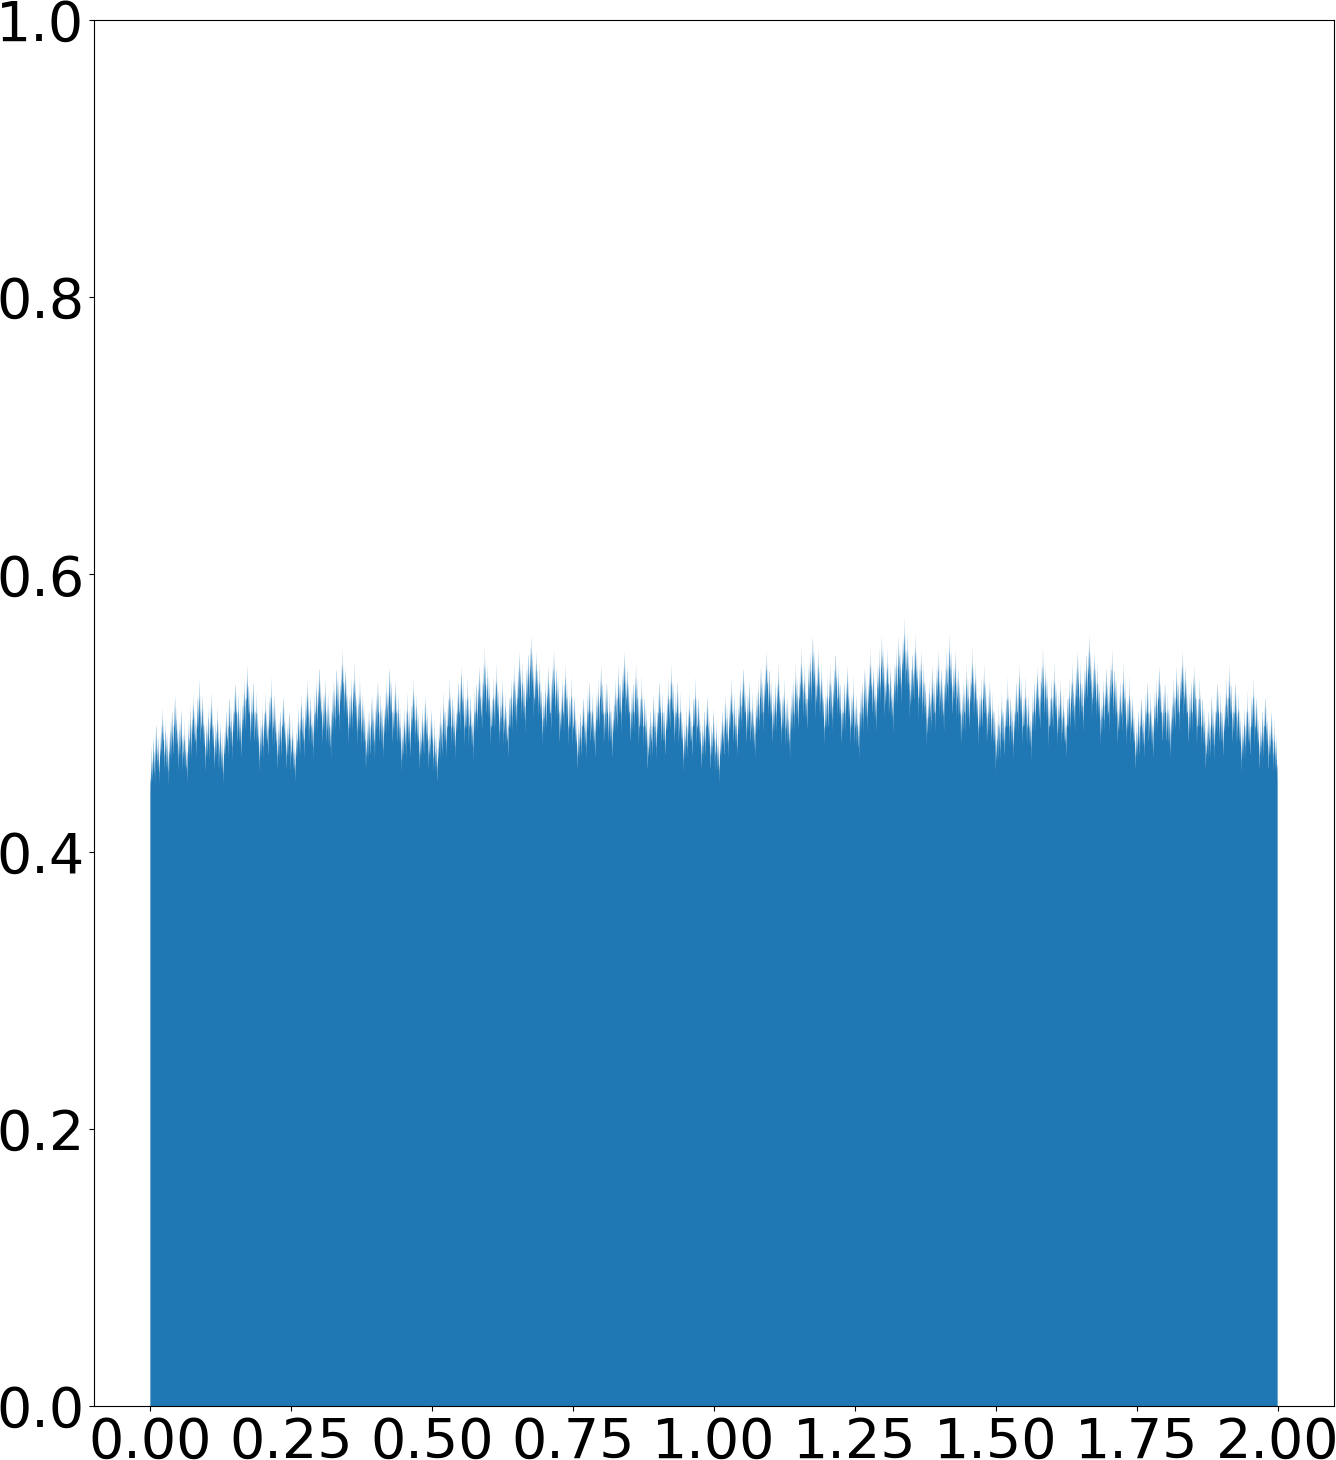
\includegraphics[width=0.48\textwidth]{figure/tent_tilted_shadow_density_0.01.png}
%%    \hspace{0.02\textwidth}
%%    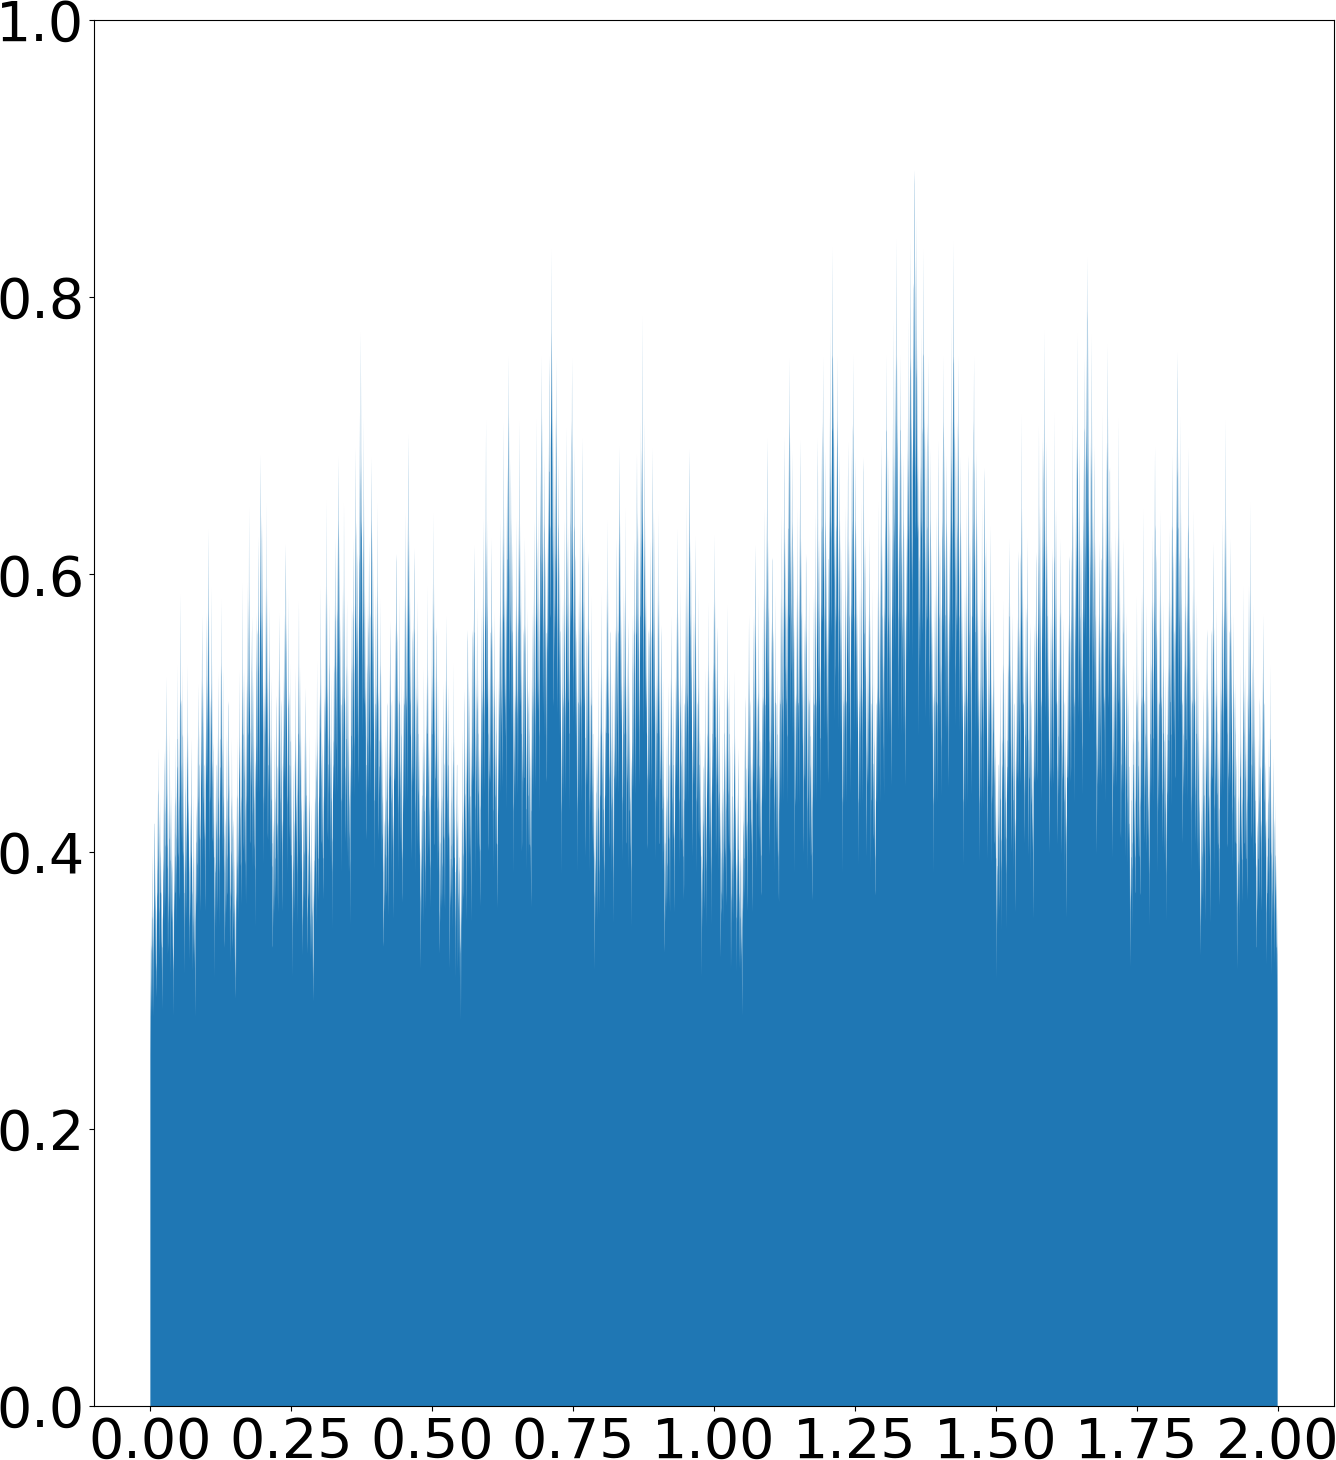
\includegraphics[width=0.48\textwidth]{figure/tent_tilted_shadow_density_0.05.png}
%%    \\ \vspace{0.02\textwidth}
%%    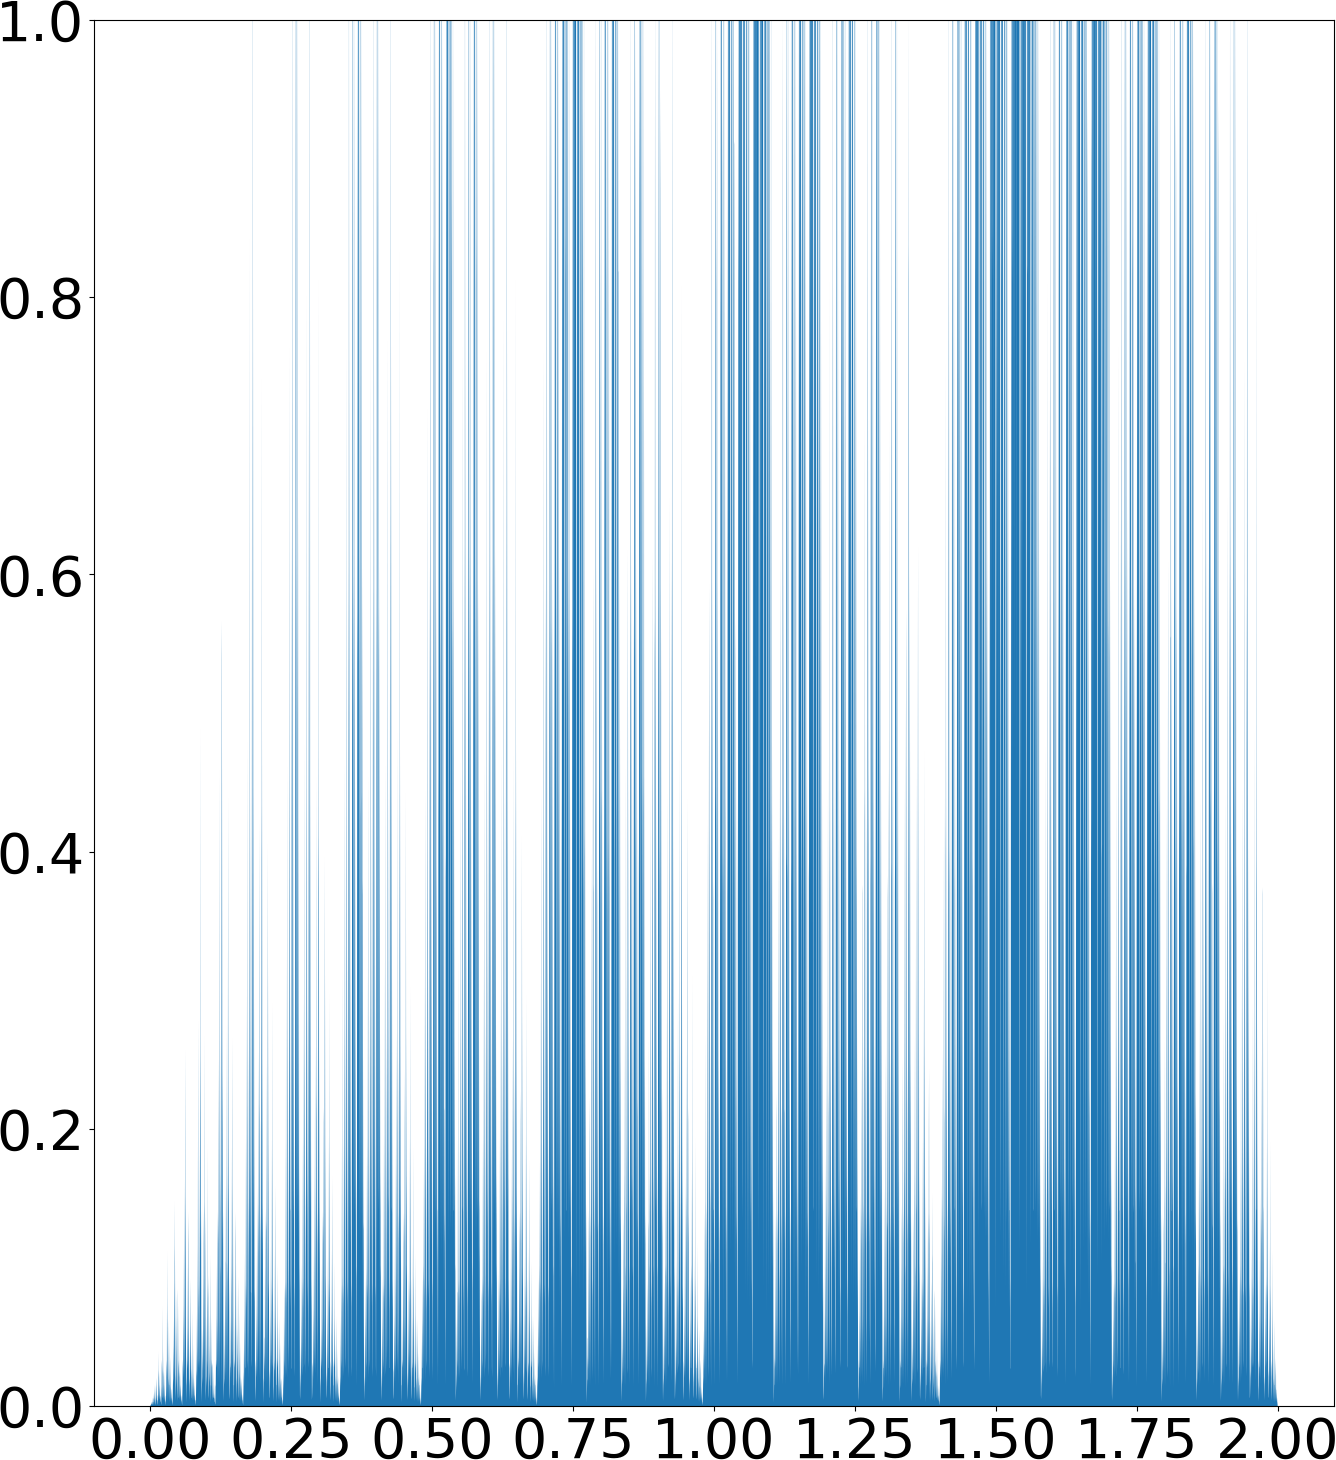
\includegraphics[width=0.48\textwidth]{figure/tent_tilted_shadow_density_0.4.png}
%%    \hspace{0.02\textwidth}
%%    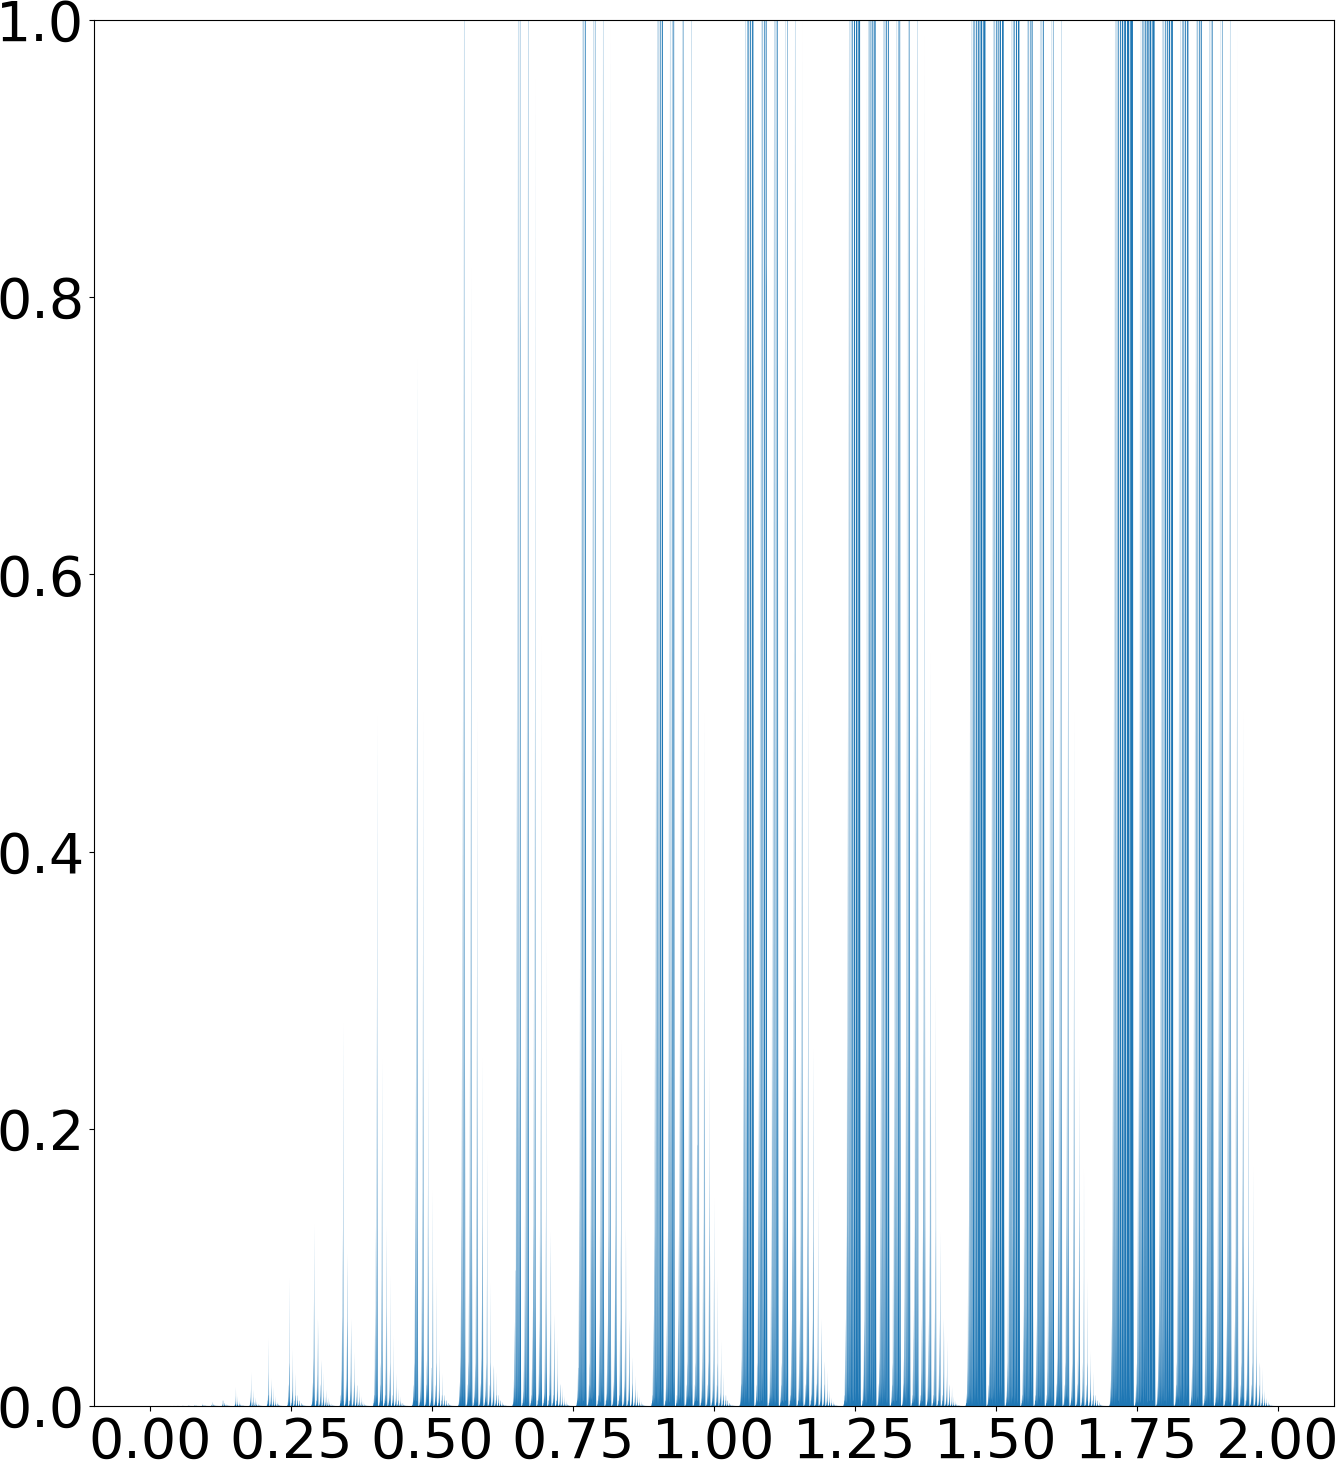
\includegraphics[width=0.48\textwidth]{figure/tent_tilted_shadow_density_0.7.png}
%%    \caption{Caption}
%%    \label{fig:tent_tilted_shadow}
%%\end{figure}
%%

\begin{figure}[H]
    \centering
    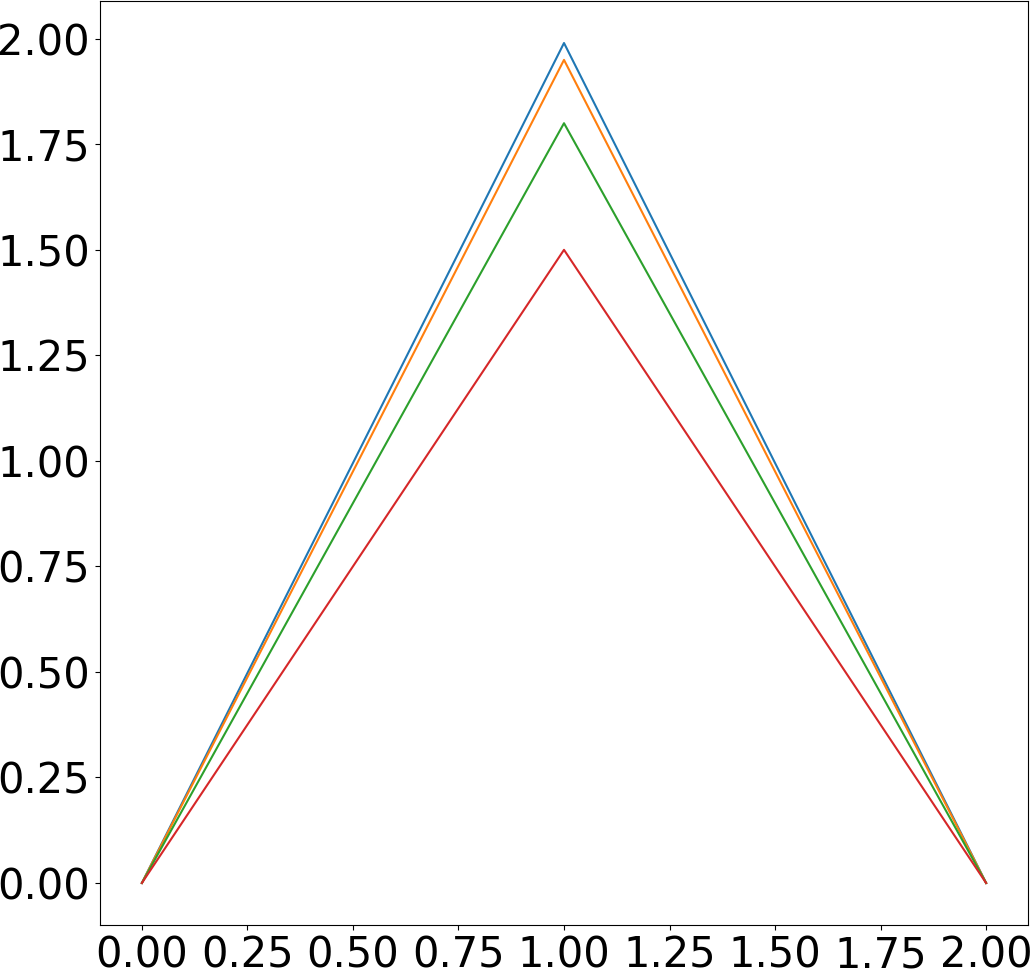
\includegraphics[width=0.48\textwidth]{figure/squashed_tent_map.png}
    \caption{The ``squashed'' tent map (Eq. \ref{eqn:tent_squashed}) for $s=0.01, 0.05, 0,2,$ and 0.5.}
    \label{fig:tent_squashed}
\end{figure}

This section attempts to answer this question by investigating several other
perturbations, the first of which scales the height, but not the width,
of the tent map.  The resulting ``squashed'' tent map, illustrated
in Figure \ref{fig:tent_squashed}, has the closed form 
\begin{equation} \label{eqn:tent_squashed}
\hat{\varphi}^{\rm sq}_s(x) := \begin{cases}
    (2-s)x \quad & x < 1 \\
    (2-s)(2 - x) \quad & x \ge 1
    \end{cases}
\end{equation}


\begin{figure}[H]
    \centering
    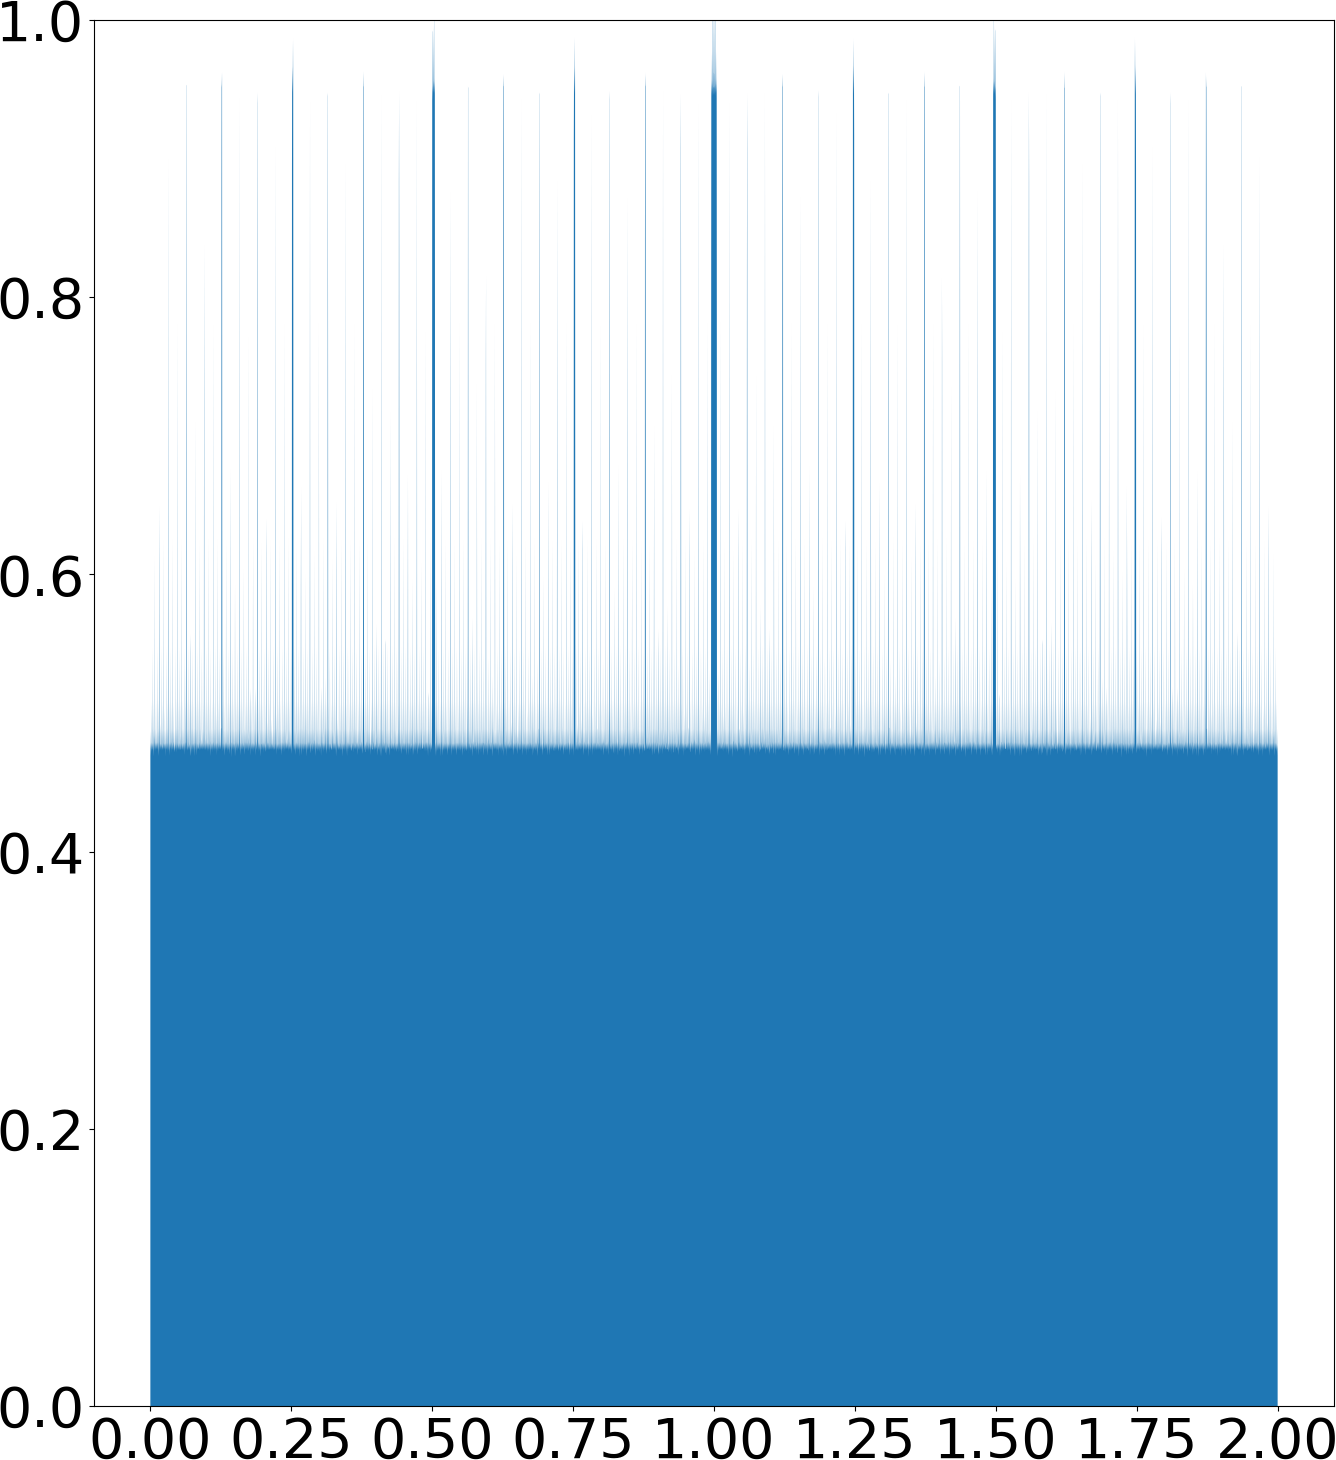
\includegraphics[width=0.48\textwidth]{figure/tent_squashed_shadow_density_0.01.png}
    \hspace{0.02\textwidth}
    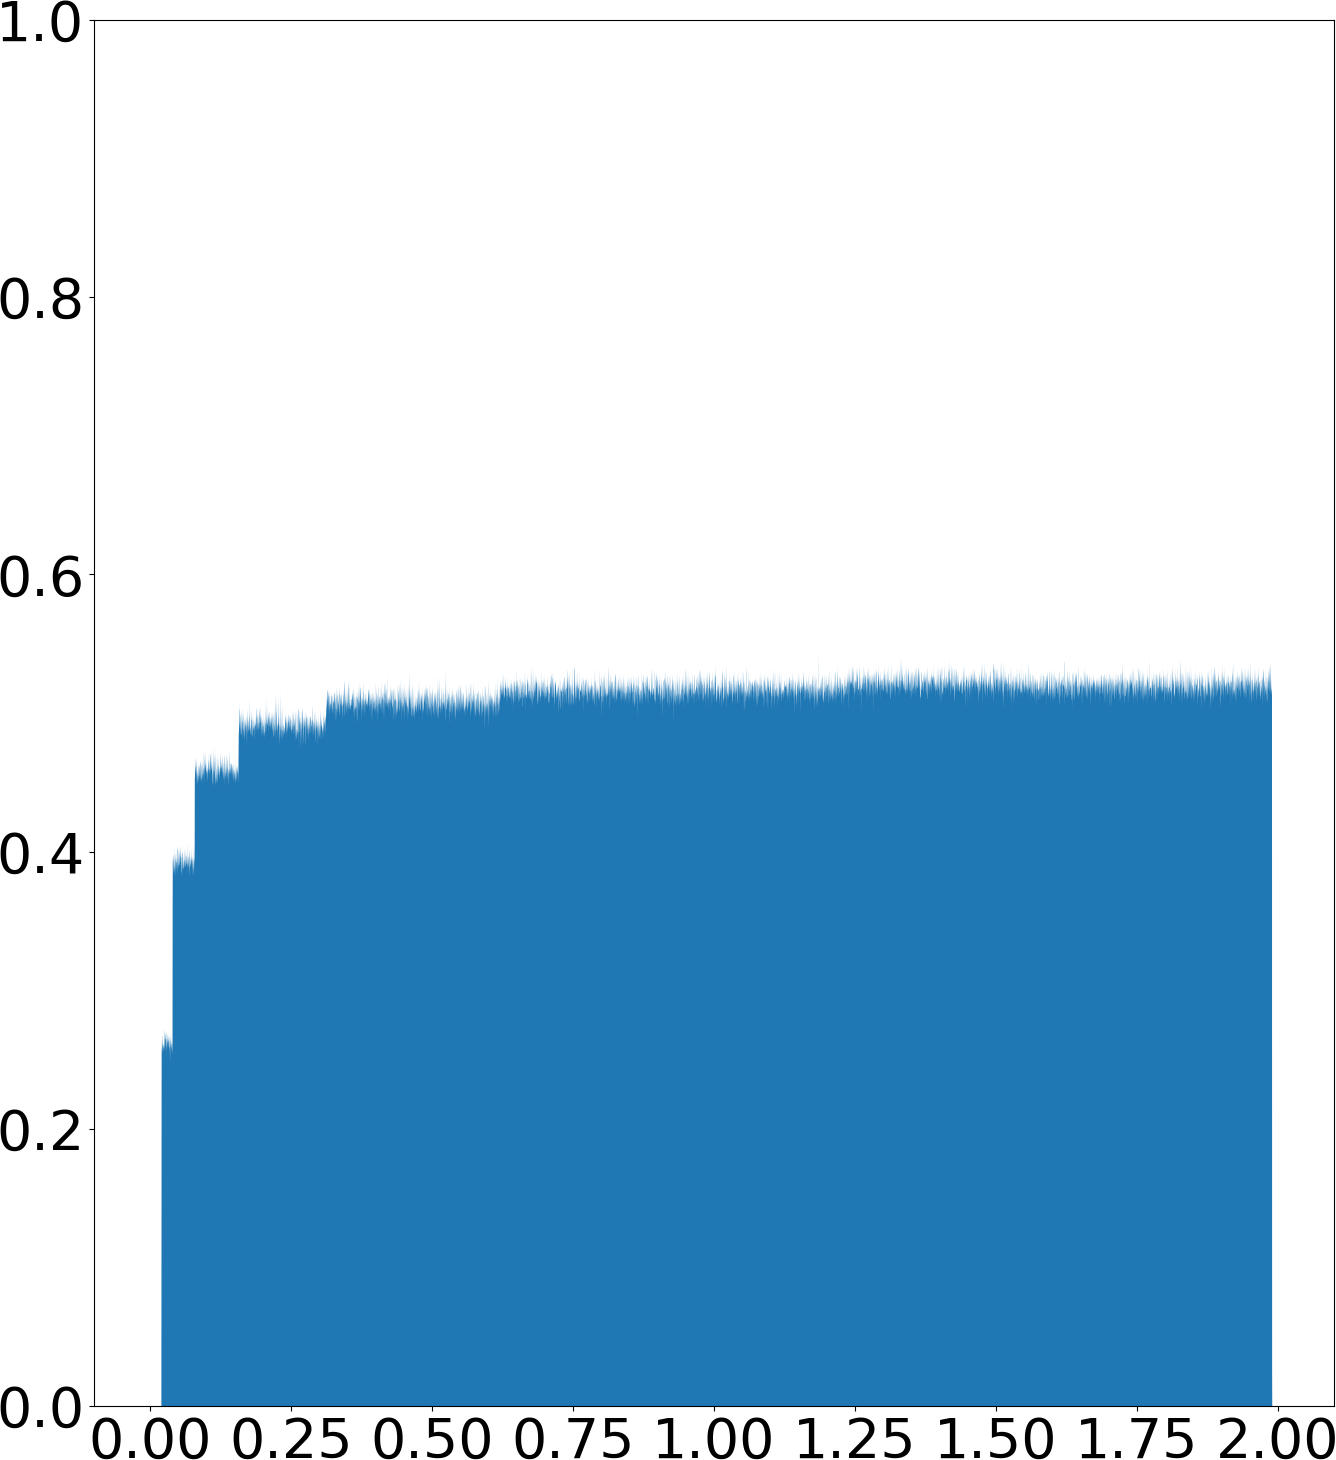
\includegraphics[width=0.48\textwidth]{figure/tent_squashed_physical_density_0.01.png}
    \\ \vspace{0.02\textwidth}
    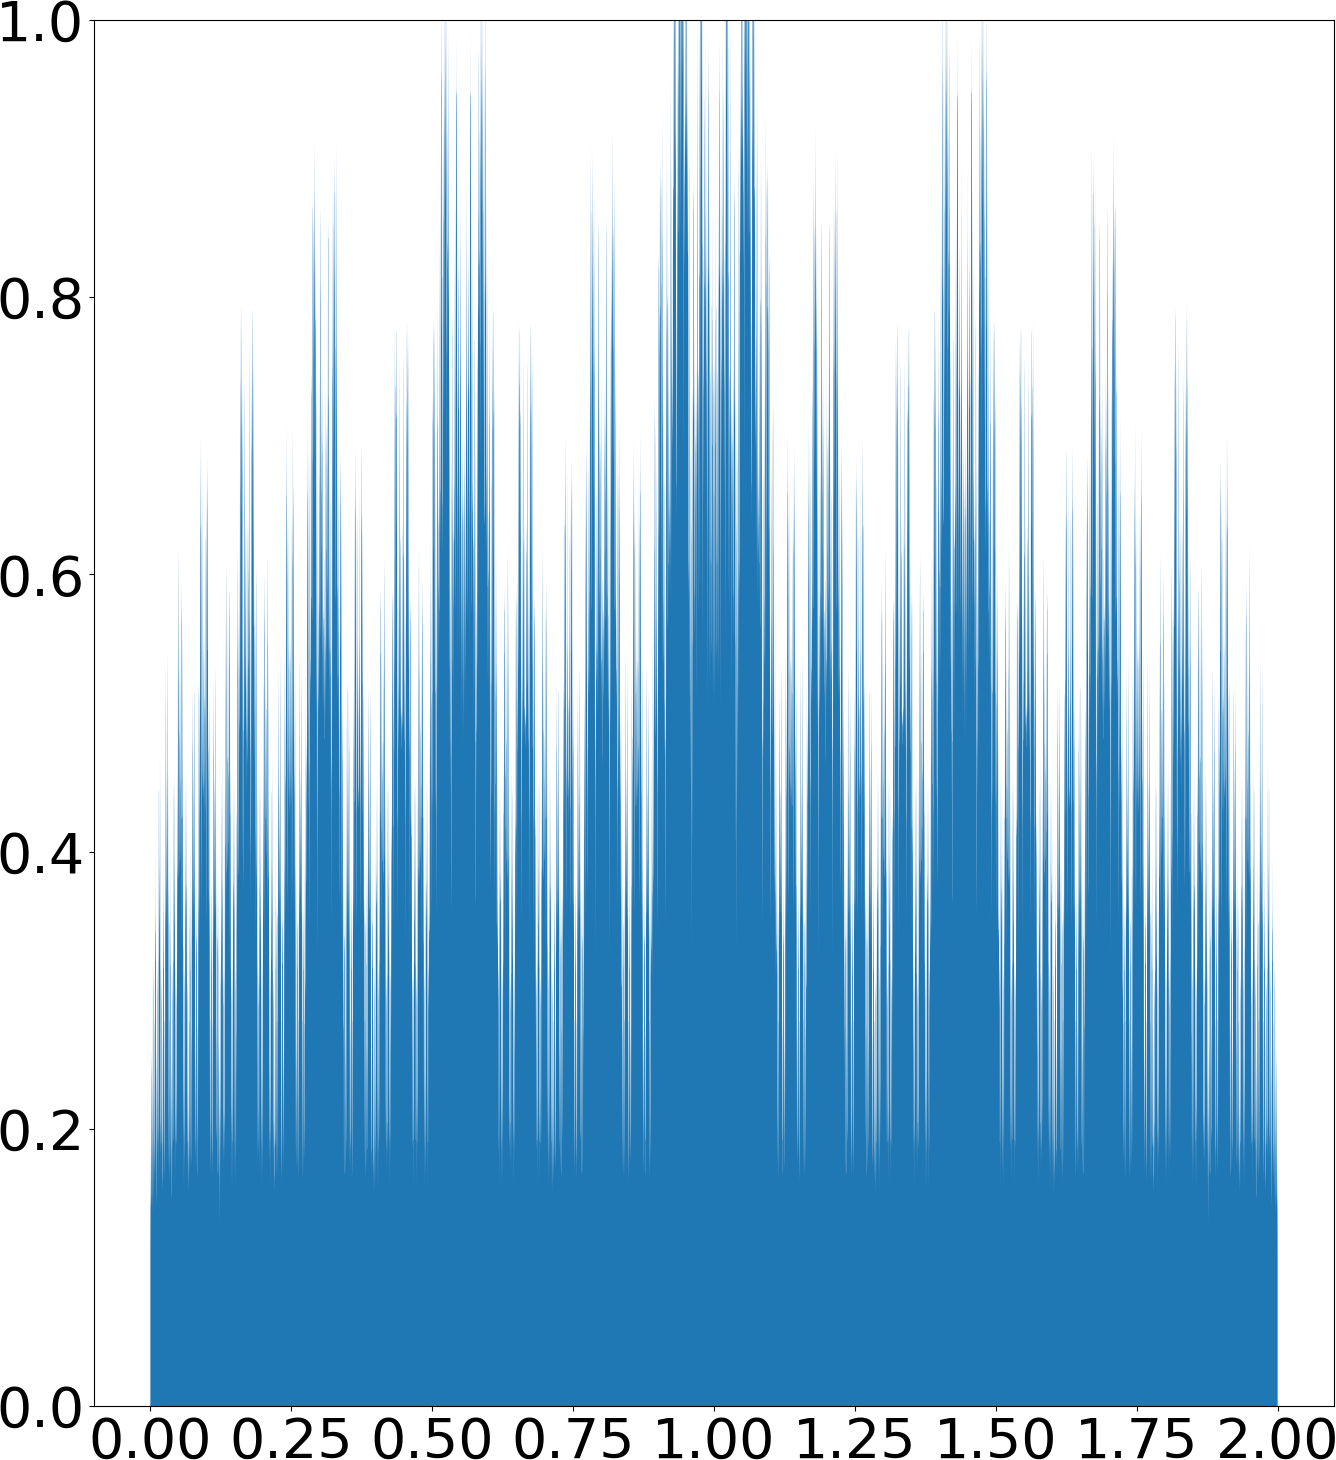
\includegraphics[width=0.48\textwidth]{figure/tent_squashed_shadow_density_0.2.png}
    \hspace{0.02\textwidth}
    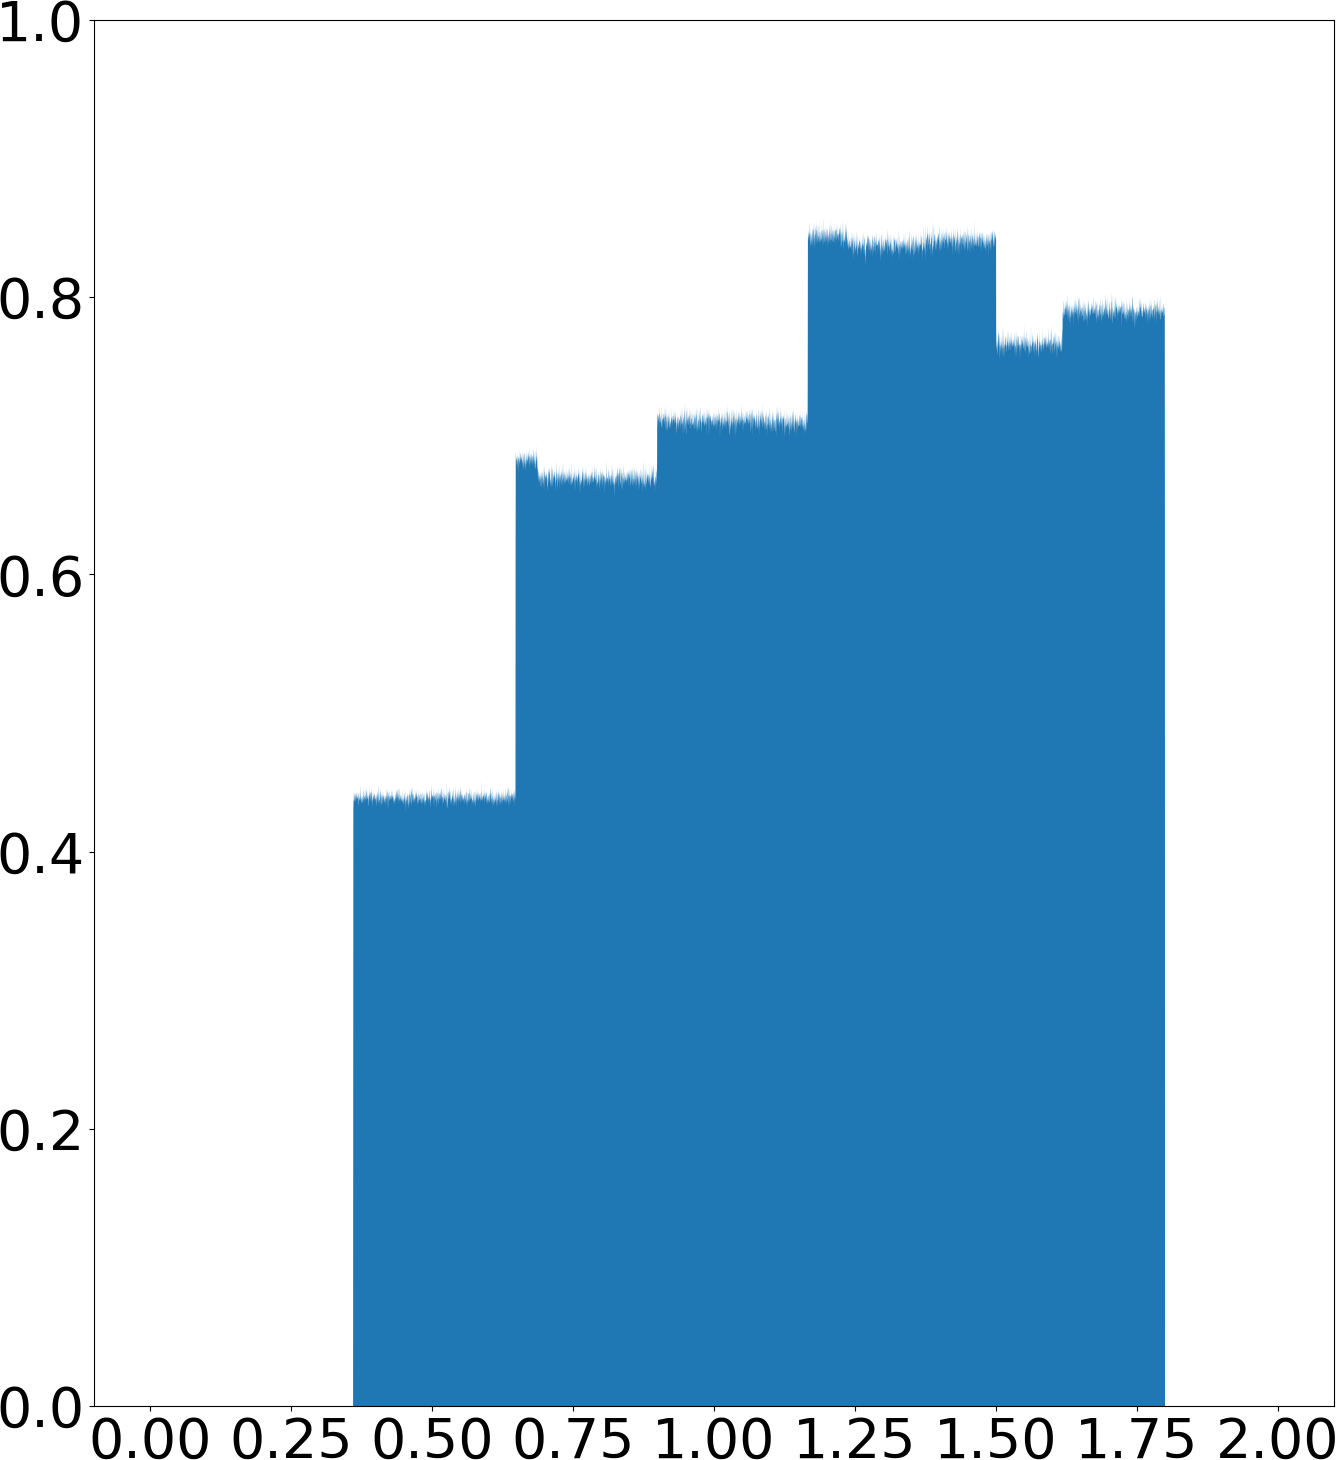
\includegraphics[width=0.48\textwidth]{figure/tent_squashed_physical_density_0.2.png}
    \caption{The left column shows the empirical distribution of the shadowing solution for the squashed tent map at $s=0.01$ (top) and at $s=0.2$ (bottom). The right column shows the probability distribution of a physical solution at the same two values of $s = 0.01$ (top) and $s = 0.2$ (bottom).}
    \label{fig:tent_squashed_shadow}
\end{figure}
In Figure \ref{fig:tent_squashed_shadow}, we show side-by-side the probability distributions generated by observing a long solution (of length 10 billion) 
of $\hat{\varphi}^{\rm sq}_s$ (left) and its corresponding shadowing solution (right)
at two different values of $s.$ The left column showing the probability distribution of the shadowing solution is reminiscent of the hairy probability distributions of 
the quasi-solutions of the tent map in Section \ref{sec:quasiphysical}. Note that, unlike the tilted tent maps, the family of squashed tent maps do not have the uniform distribution as their SRB distribution, as indicated on the right column. However, the SRB distributions are not fractal. That is, the physical solutions of the squashed tent map are distributed according to a regular probability density (right column of Figure \ref{fig:tent_squashed_shadow}). But the shadowing solution, which is a true orbit of the original tent map, is distributed neither like a physical solution of the original tent map nor of the squashed tent map, as suggested by its fractal-like empirical probability distribution. 

Next we consider a second perturbation of the tent map, the \emph{pinched} tent map, which has the following closed form
\begin{align}
    \hat{\varphi}^p_s(x) = \begin{cases}
        \dfrac{4x}{1 + s + \sqrt{(1+s)^2 - 4s x} }, & x < 1 \\
        \dfrac{4(2-x)}{1 + s + \sqrt{(1+s)^2 - 4s(2- x)} }, & 2 \leq x \leq 1.
    \end{cases}
    \label{eqn:tent_pinched}
\end{align}
Again, at $s=0$, the original tent map is recovered, and other values of $s,$ the tent map is ``pinched'' by perturbations that are symmetric around $x = 1$, and zero at the end points. Figure \ref{fig:tent_pinched} shows the pinched tent map at different $s$ values.  
\begin{figure}[H]
    \centering
    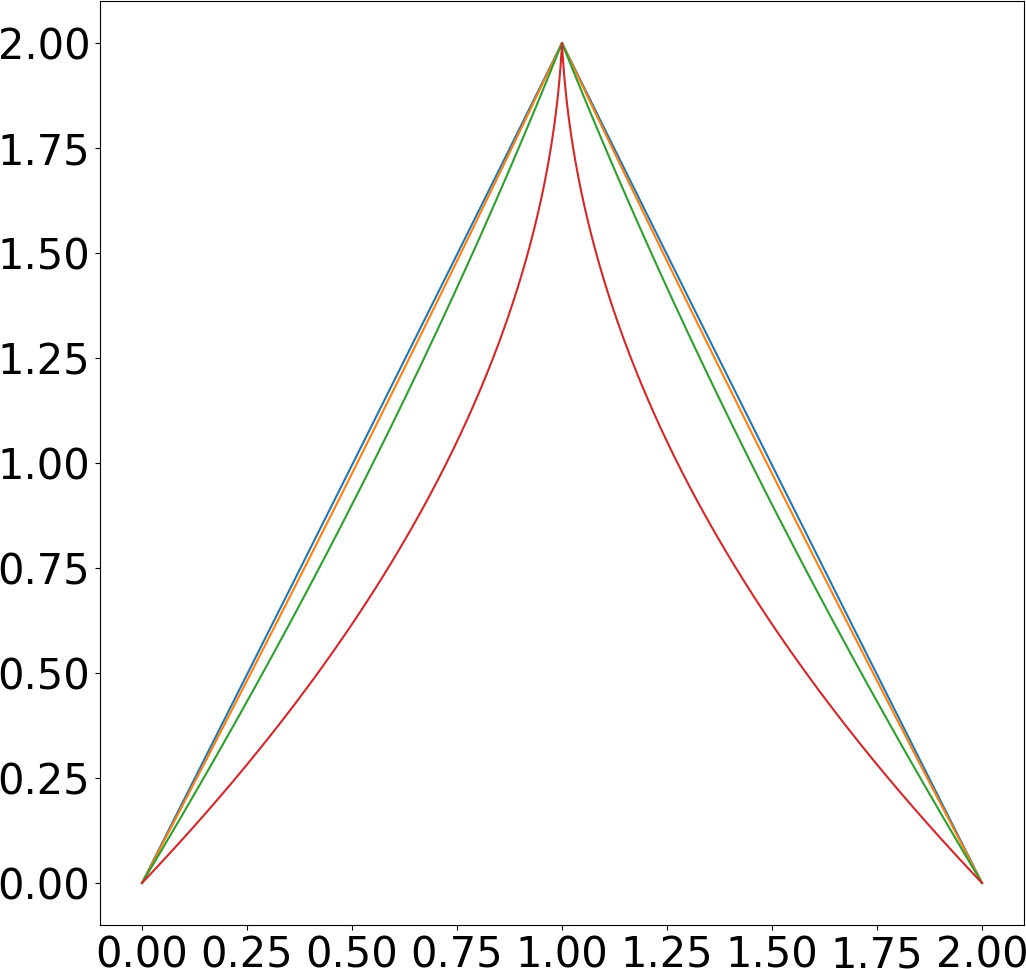
\includegraphics[width=0.48\textwidth]{figure/pinched_tent_map.png}
    \caption{The pinched tent map (Eq. \ref{eqn:tent_pinched}) for $s = 0.01, 0.05, 0.2,$ and 0.5.}
    \label{fig:tent_pinched}
\end{figure}
In Figure \ref{fig:tent_pinched_shadow}, we show the corresponding plots of the 
physical and shadowing distributions for the pinched tent map. From the right 
column, which shows the probability density of a long physical solution, we 
can see that the pinching perturbation changes the uniform density of the original tent map to a linearly varying density. The more pronounced the perturbation -- the higher the value of $s$ -- the steeper decline in the density from left to the right. The shadowing distribution, in this case as well, appears fractal. Once again, with probability one -- or, for any randomly chosen initial condition of the solution of the pinched tent map -- any physical solution is shadowed by a quasi-physical solution.
\begin{figure}[H]
    \centering
    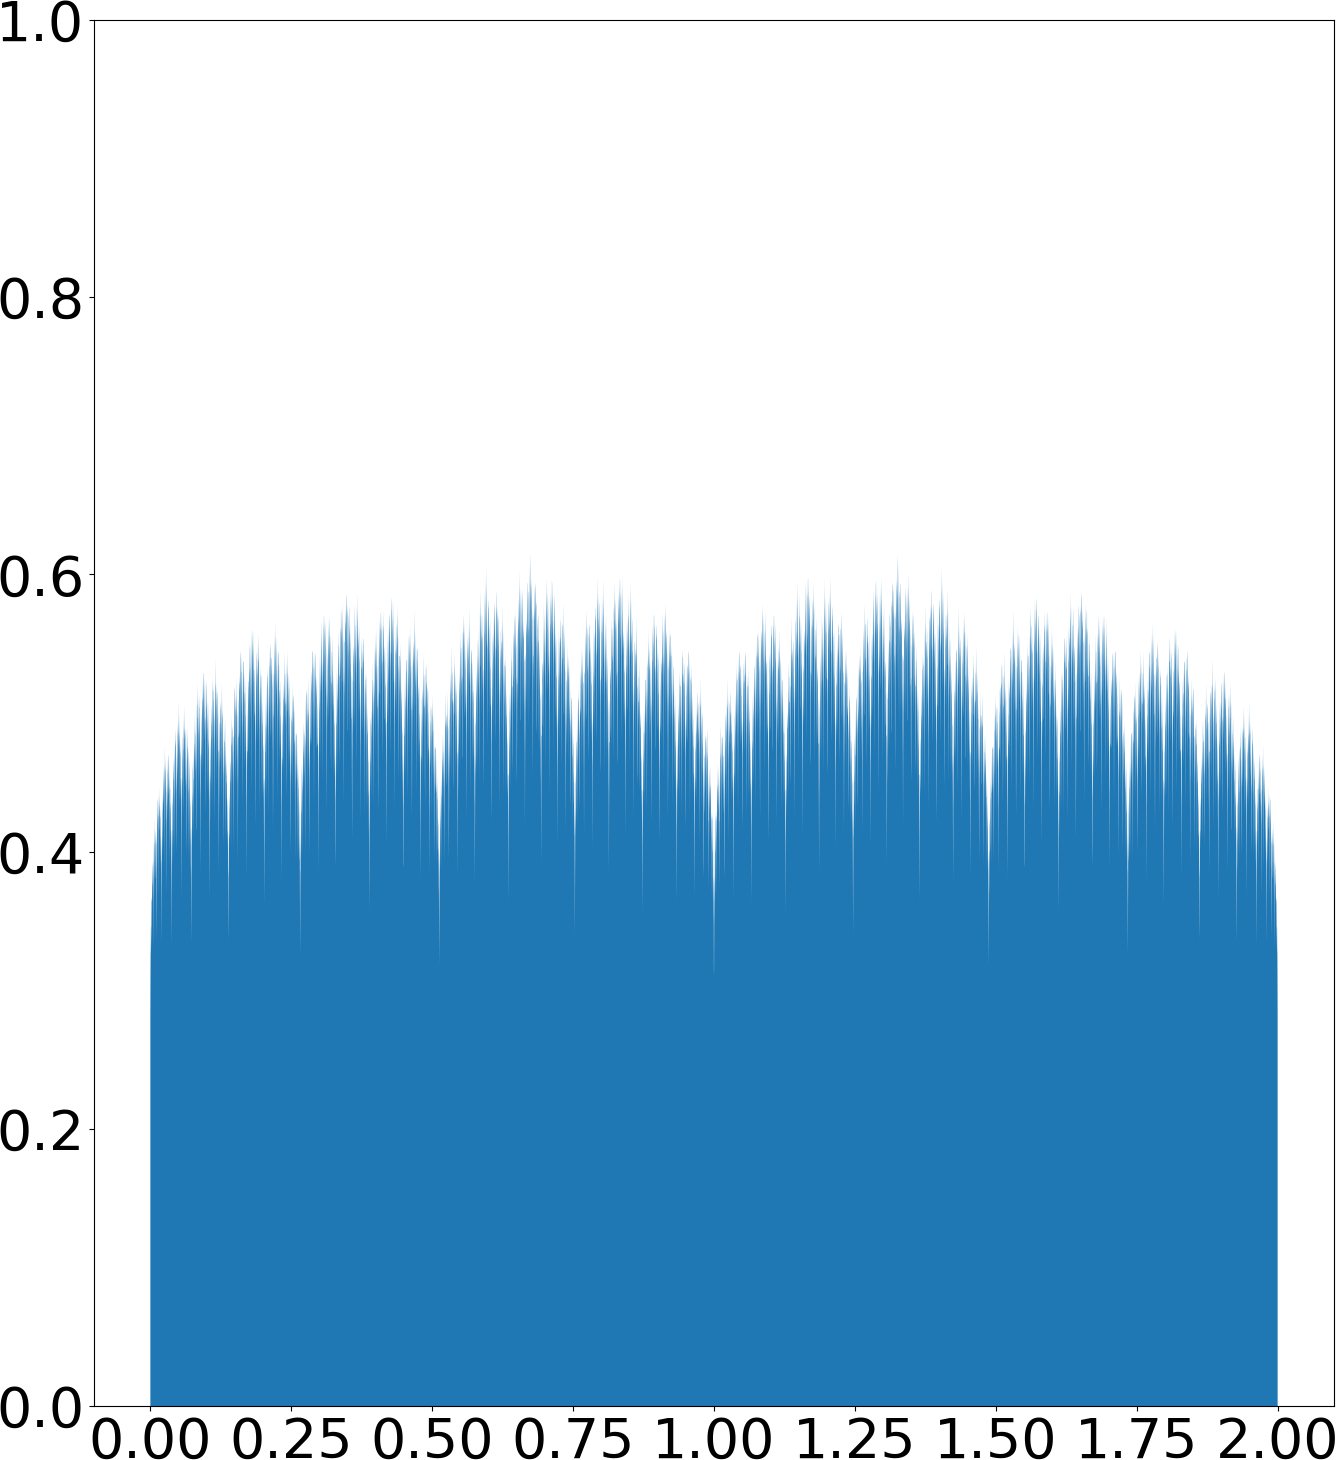
\includegraphics[width=0.48\textwidth]{figure/tent_pinched_shadow_density_0.05.png}
    \hspace{0.02\textwidth}
    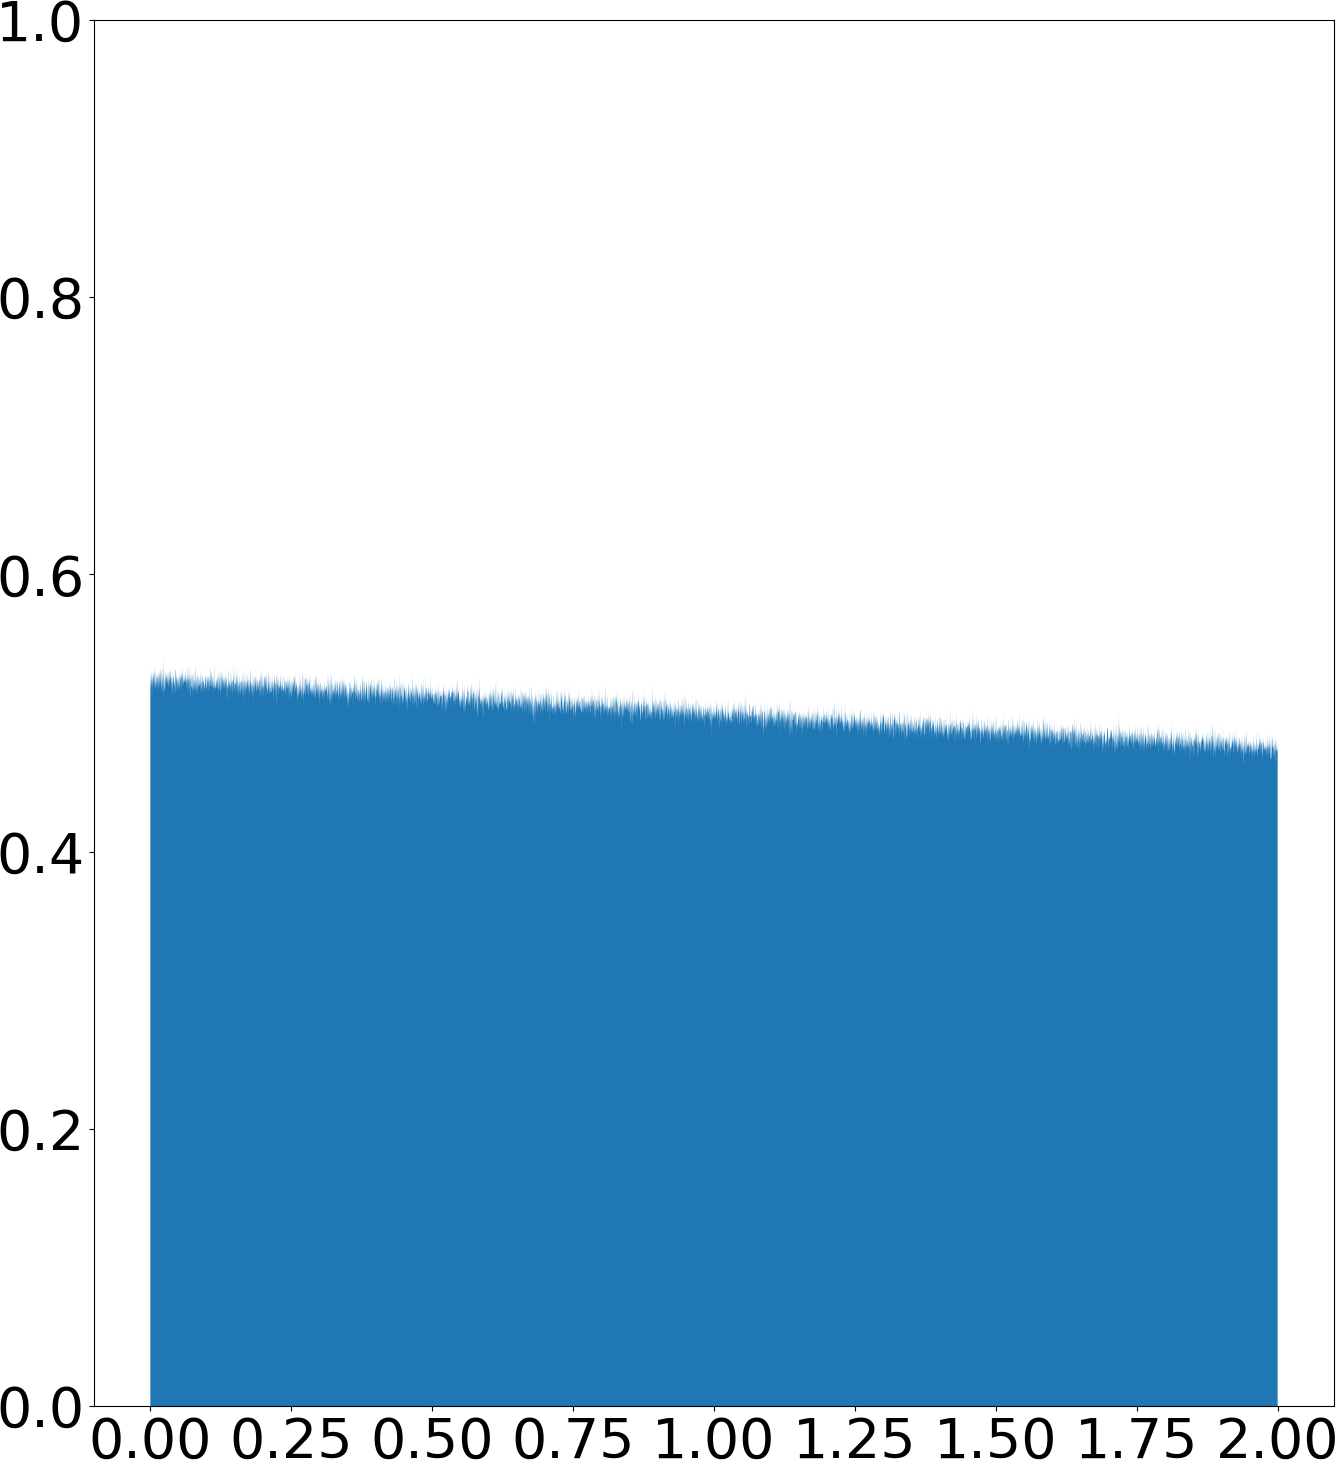
\includegraphics[width=0.48\textwidth]{figure/tent_pinched_physical_density_0.05.png}
    \\ \vspace{0.02\textwidth}
    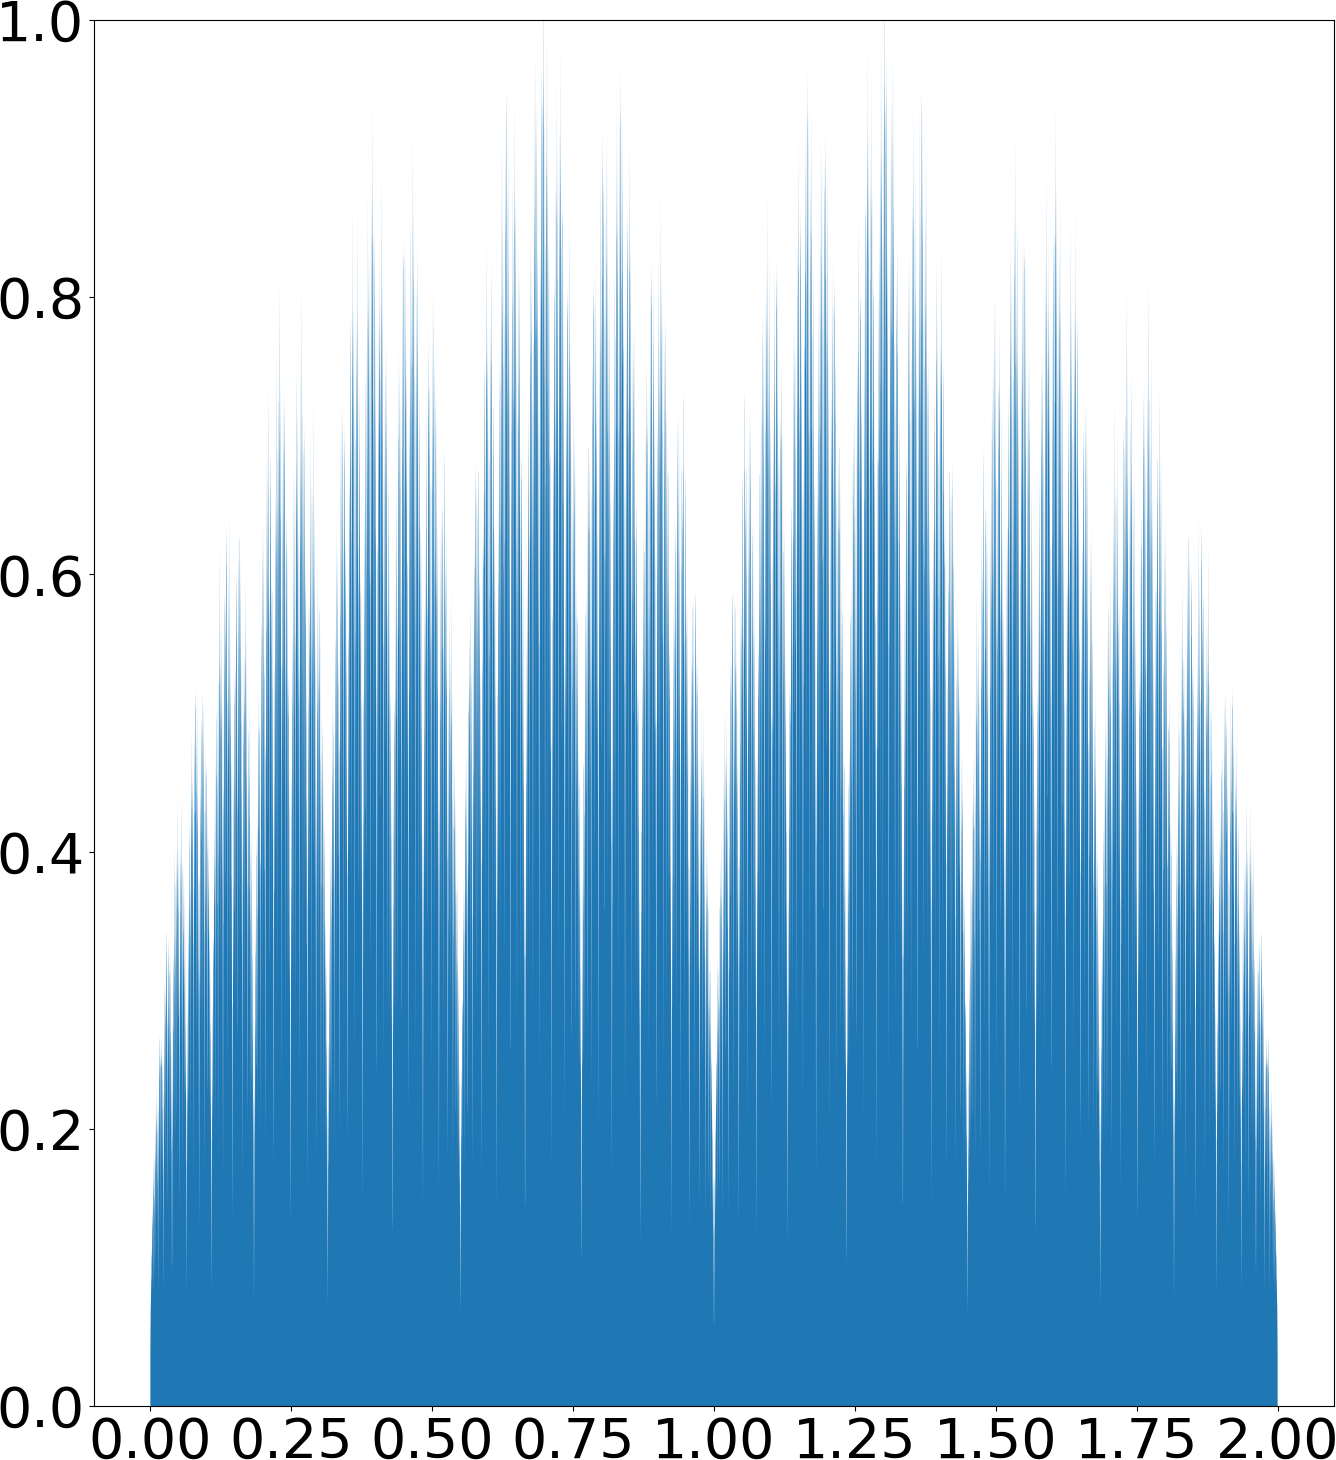
\includegraphics[width=0.48\textwidth]{figure/tent_pinched_shadow_density_0.2.png}
    \hspace{0.02\textwidth}
    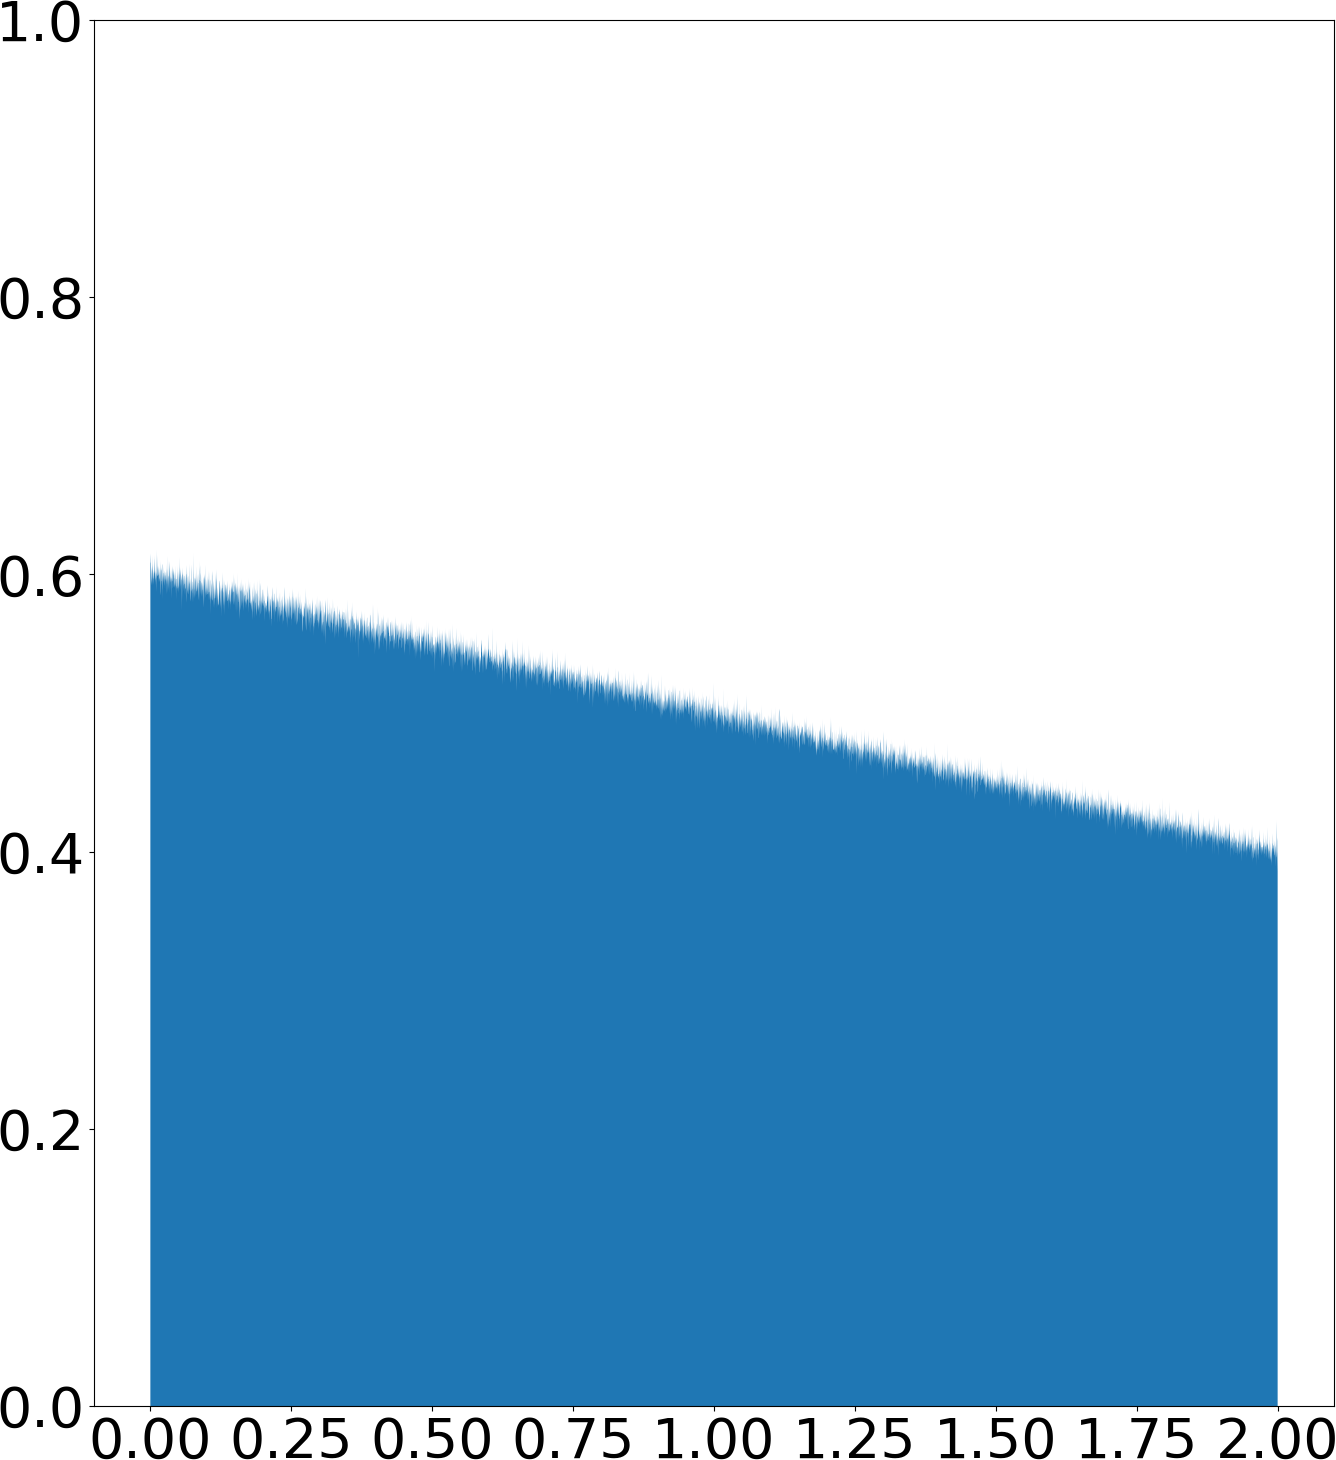
\includegraphics[width=0.48\textwidth]{figure/tent_pinched_physical_density_0.2.png}
    \caption{The left column shows the empirical distribution of the shadowing solution for the pinched tent map at $s=0.05$ (top) and at $s=0.2$ (bottom). The right column shows the probability distribution of a physical solution at the same two values of $s = 0.05$ (top) and $s = 0.2$ (bottom).}
    \label{fig:tent_pinched_shadow}
\end{figure}
We consider yet another perturbation of the tent map with the closed form
\begin{align}
\hat{\varphi}^w_s(x) = \begin{cases}
        \dfrac{4x}{1 + s + \sqrt{(1+s)^2 - 4s x} }, & x < 1 \\
        \dfrac{4(2-x)}{1 - s + \sqrt{(1-s)^2 - 4s(2- x)} }, & 2 \leq x \leq 1.
    \end{cases}
    \label{eqn:tent_wave}
\end{align}
The above map, called the wave tent map, is illustrated in Figure \ref{fig:tent_wave}.
To construct the pinched tent map (Eq. \ref{eqn:tent_pinched}), we perturbed the original tent map in such a way that the perturbations on the two halves of the interval $[0,2]$ are mirror images of each other about the $x=1$ line. In the wave tent map, the perturbations on the two halves are a reflection of each other about the 
$x$-axis.
\begin{figure}[H]
    \centering
    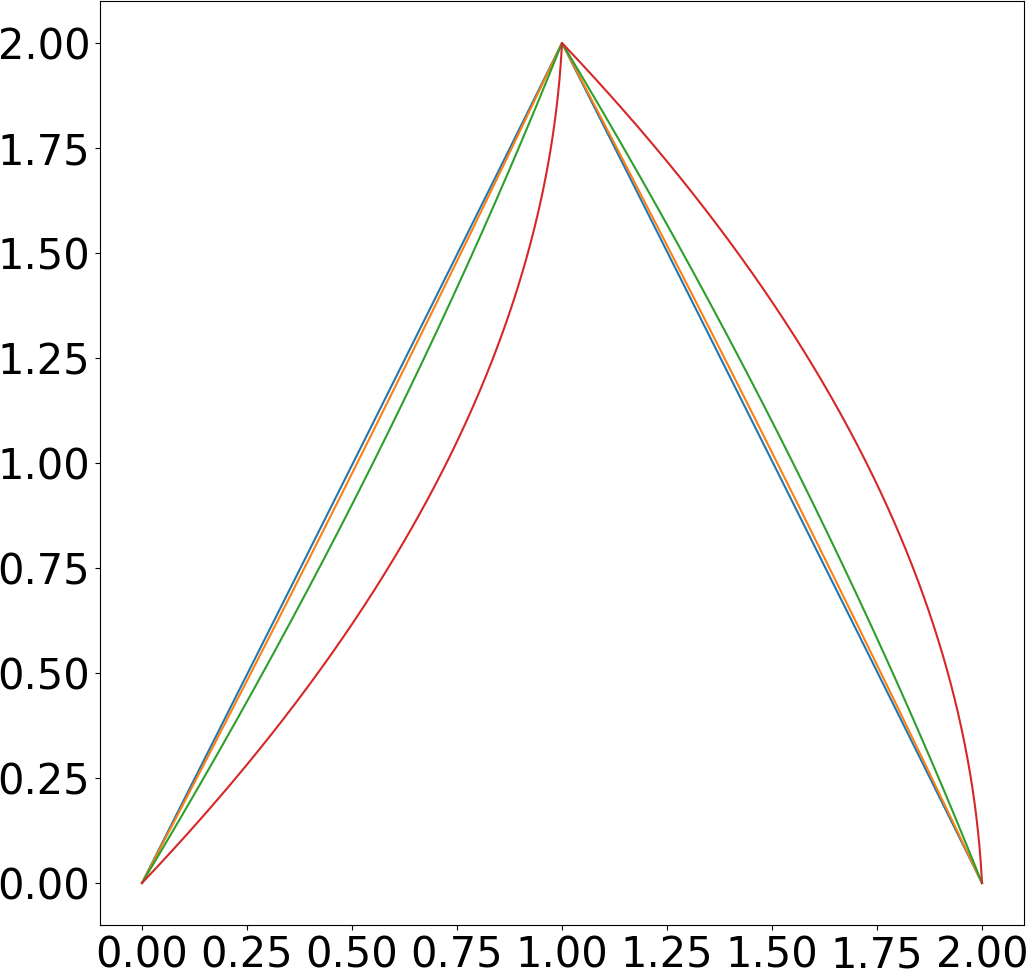
\includegraphics[width=0.48\textwidth]{figure/wave_tent_map.png}
    \caption{The wave tent map (Eq. \ref{eqn:tent_wave}) for $s = 0.01, 0.05, 0.2,$ and 0.5.}
    \label{fig:tent_wave}
\end{figure}
The wave perturbation does not noticeably alter the SRB density of the original tent map. As we show in Figure \ref{fig:tent_wave_shadow} (right), a solution of the 
wave tent map, starting from almost any point on $[0,2]$ -- a physical solution -- has a density that looks almost identical to a uniform density of 0.5. On the left column of Figure \ref{fig:tent_wave_shadow}, we observe that the distributions of the shadowing solutions corresponding to the physical solutions on the right, once again appear fractal.  
\begin{figure}[H]
    \centering
    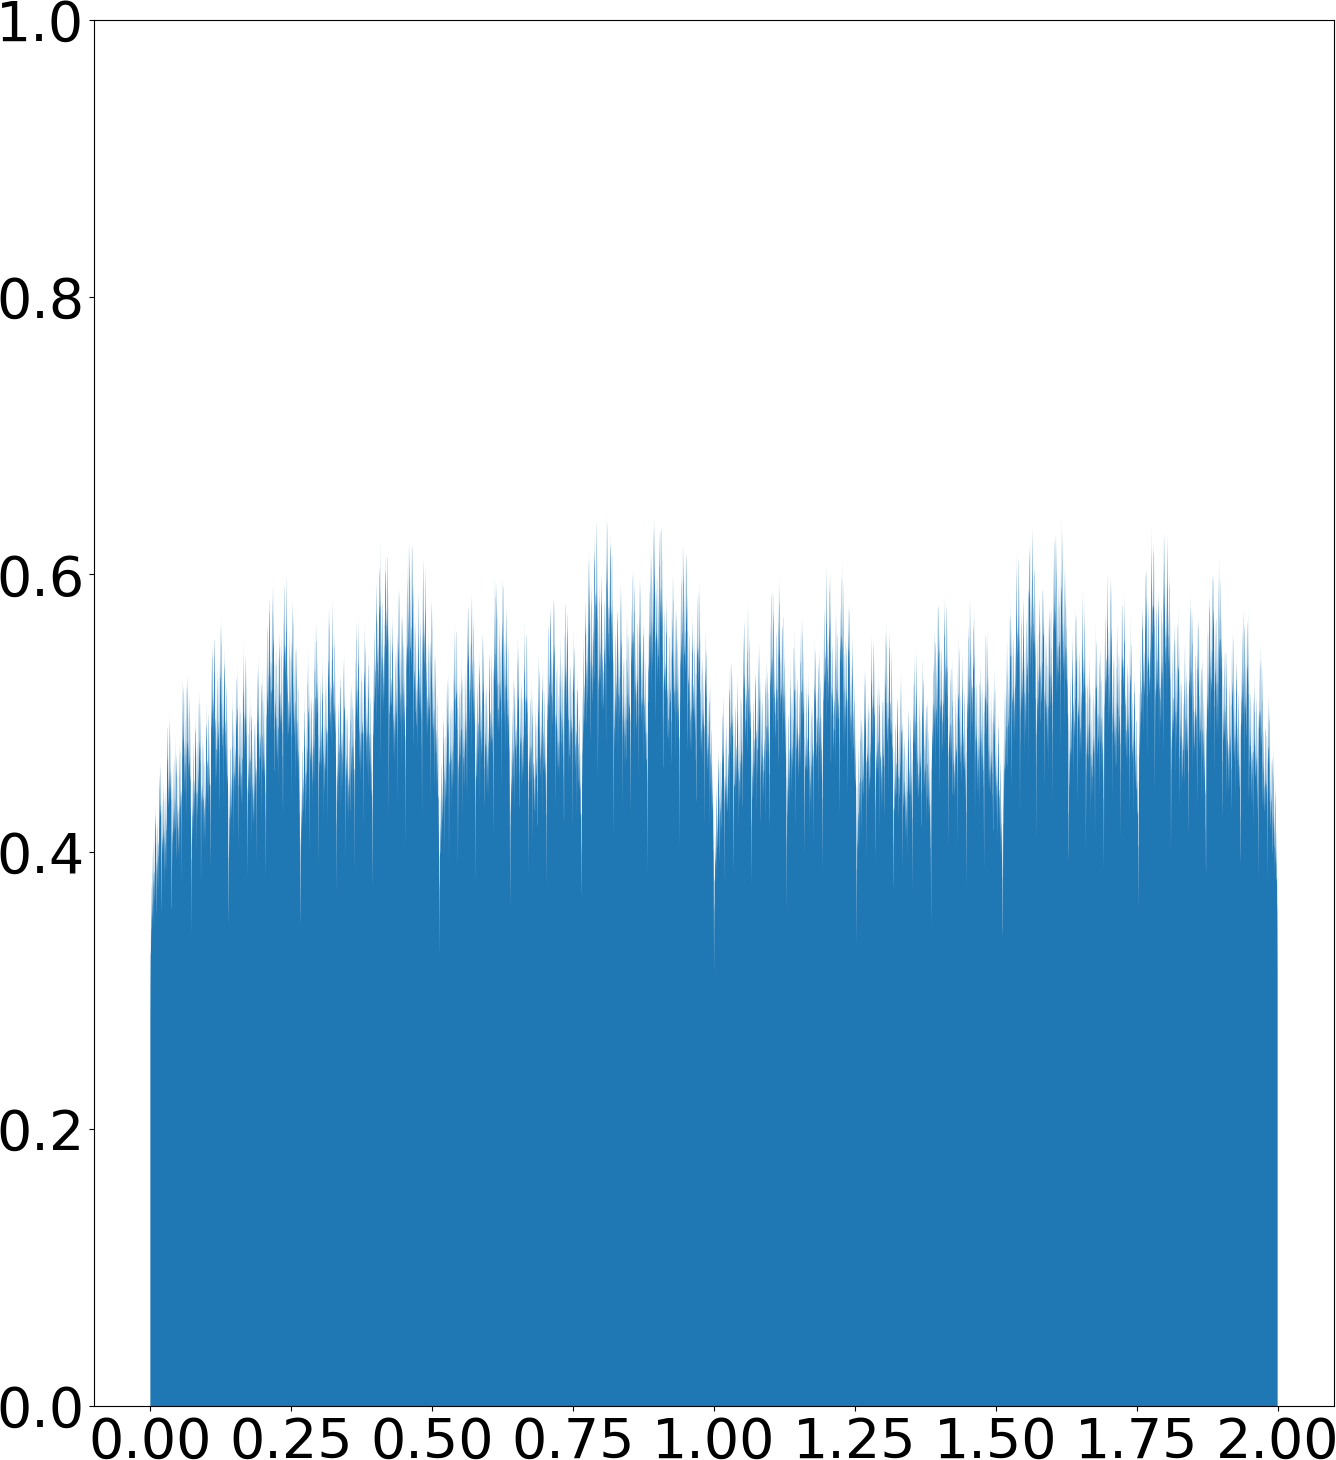
\includegraphics[width=0.48\textwidth]{figure/tent_wave_shadow_density_0.05.png}
    \hspace{0.02\textwidth}
    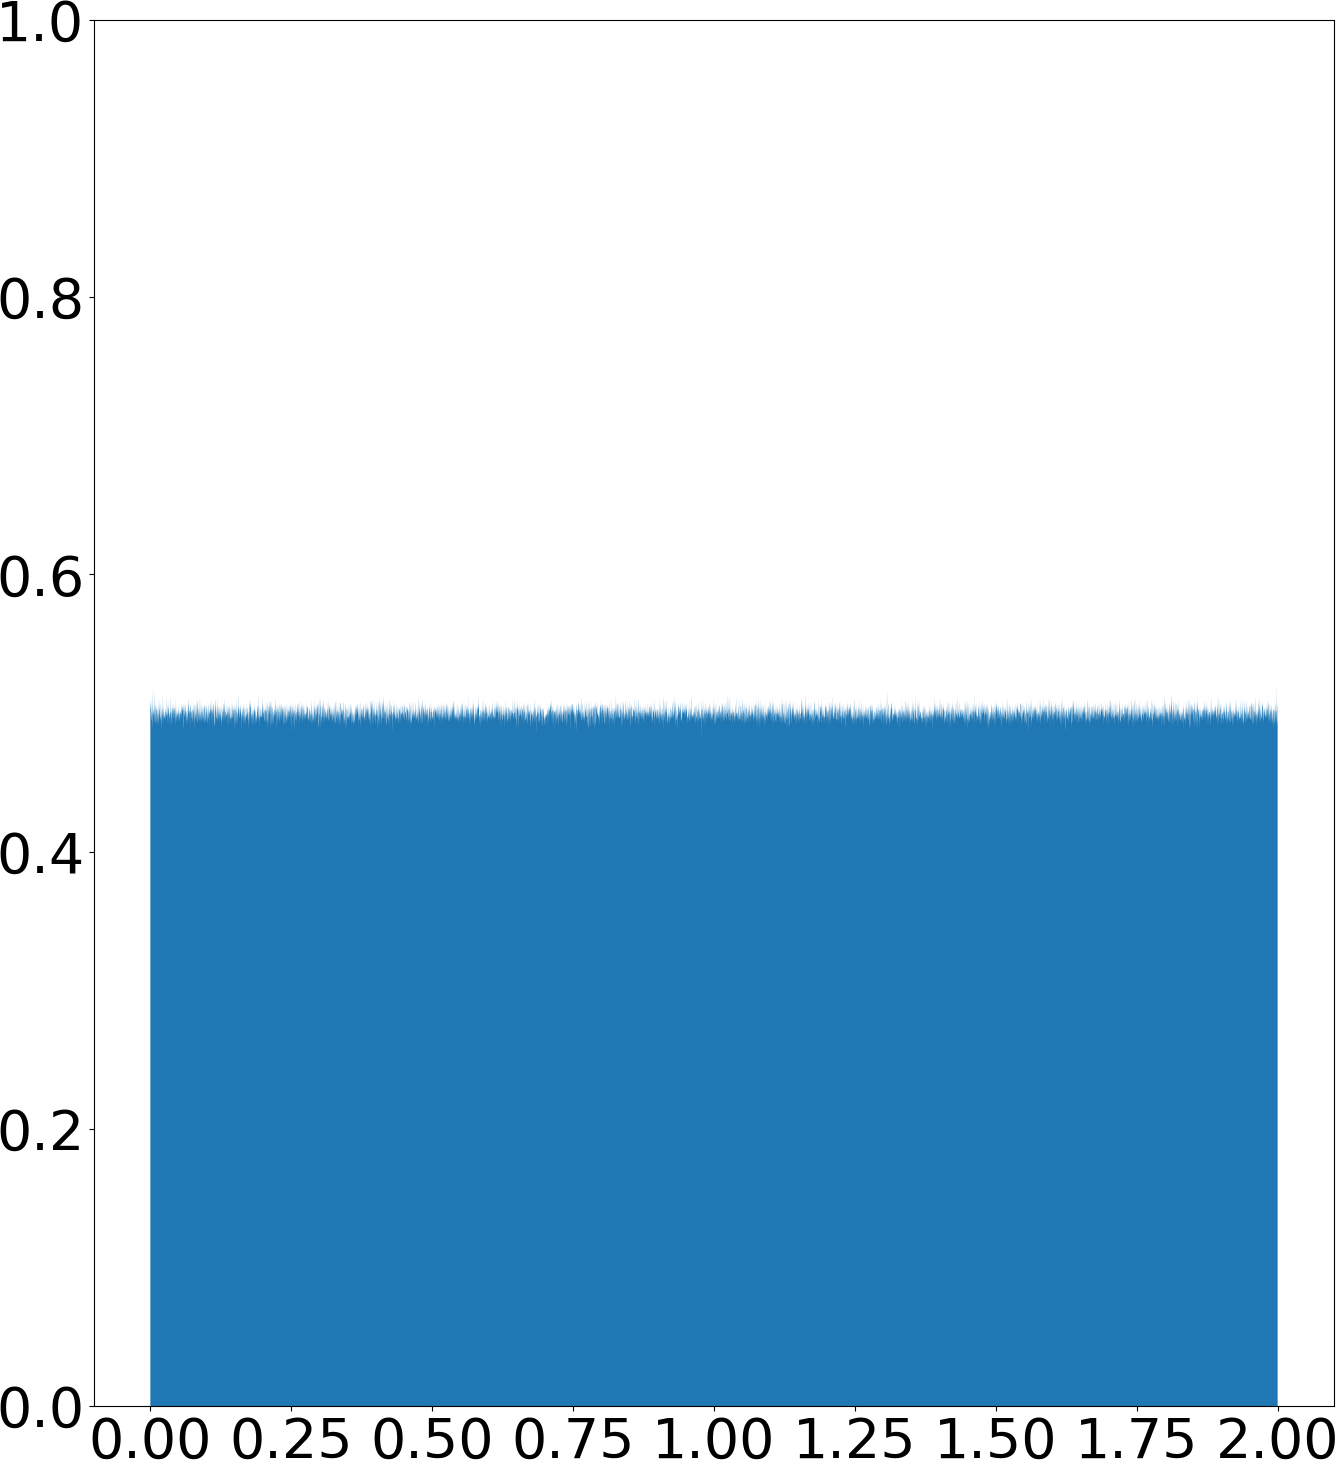
\includegraphics[width=0.48\textwidth]{figure/tent_wave_physical_density_0.05.png}
    \\ \vspace{0.02\textwidth}
    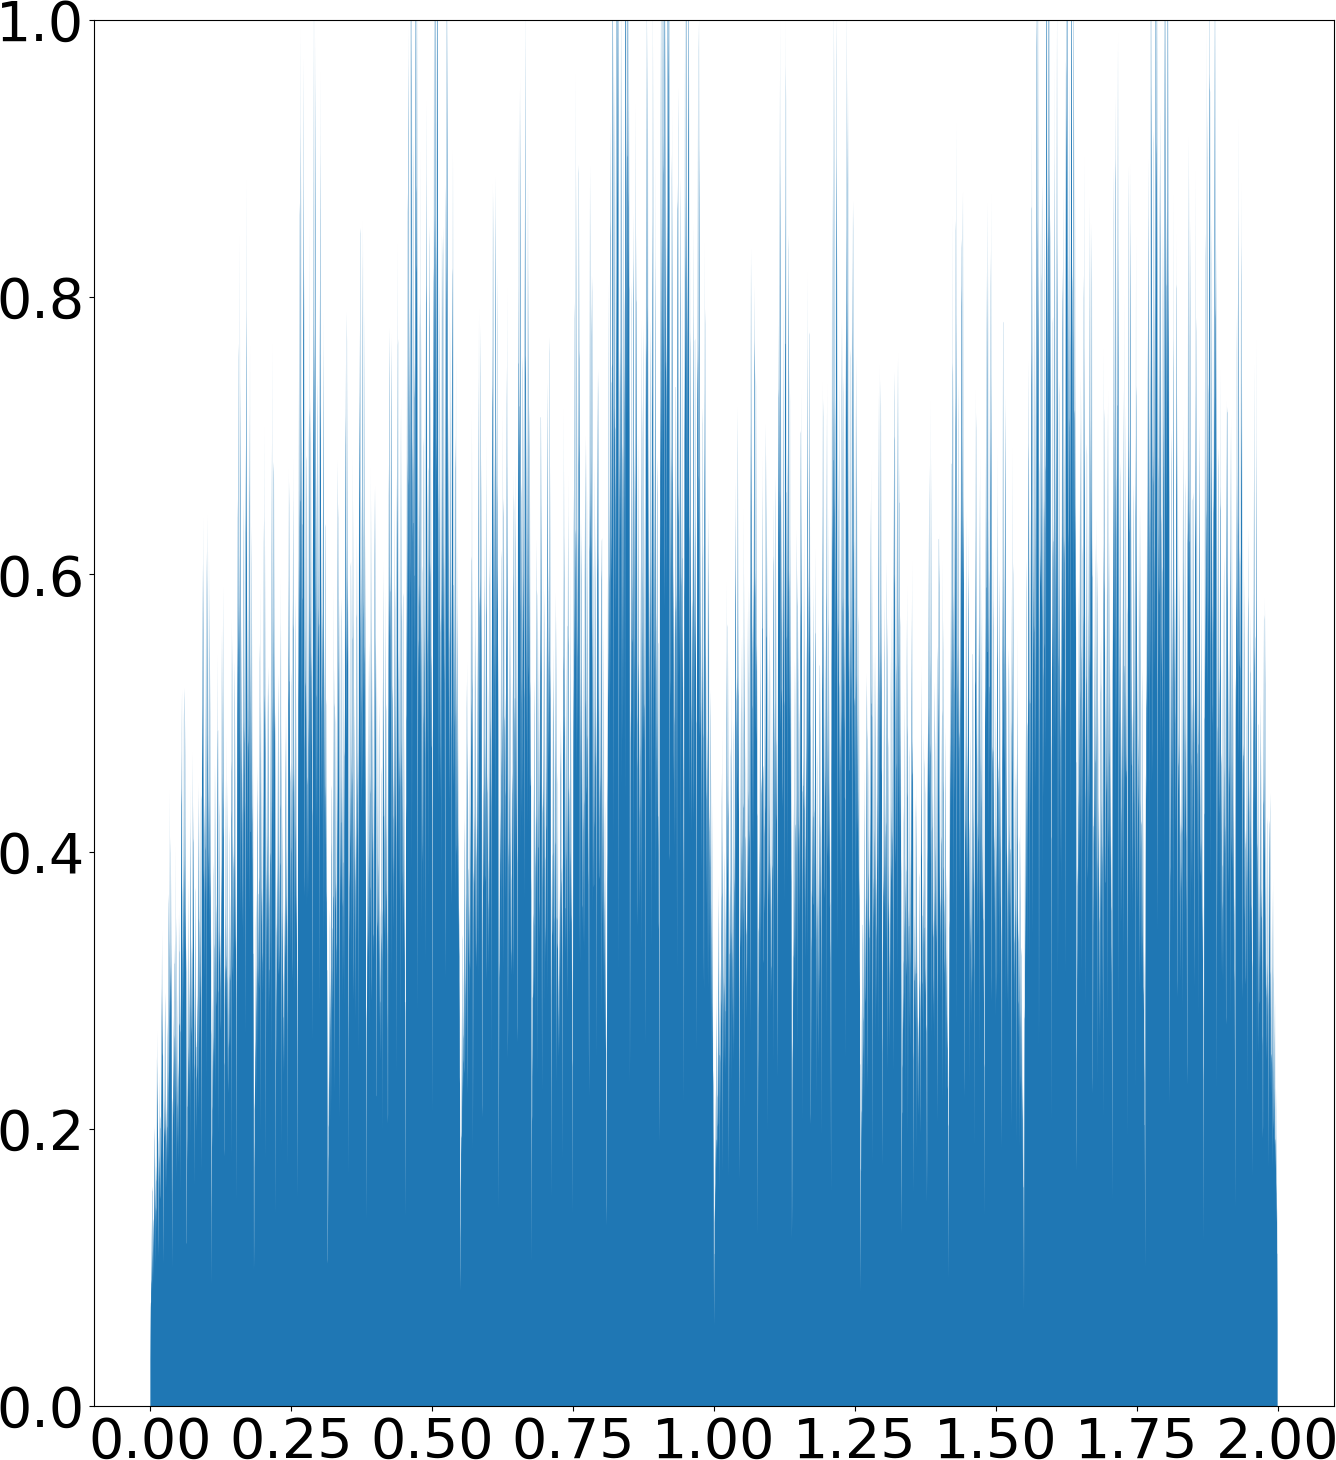
\includegraphics[width=0.48\textwidth]{figure/tent_wave_shadow_density_0.2.png}
    \hspace{0.02\textwidth}
    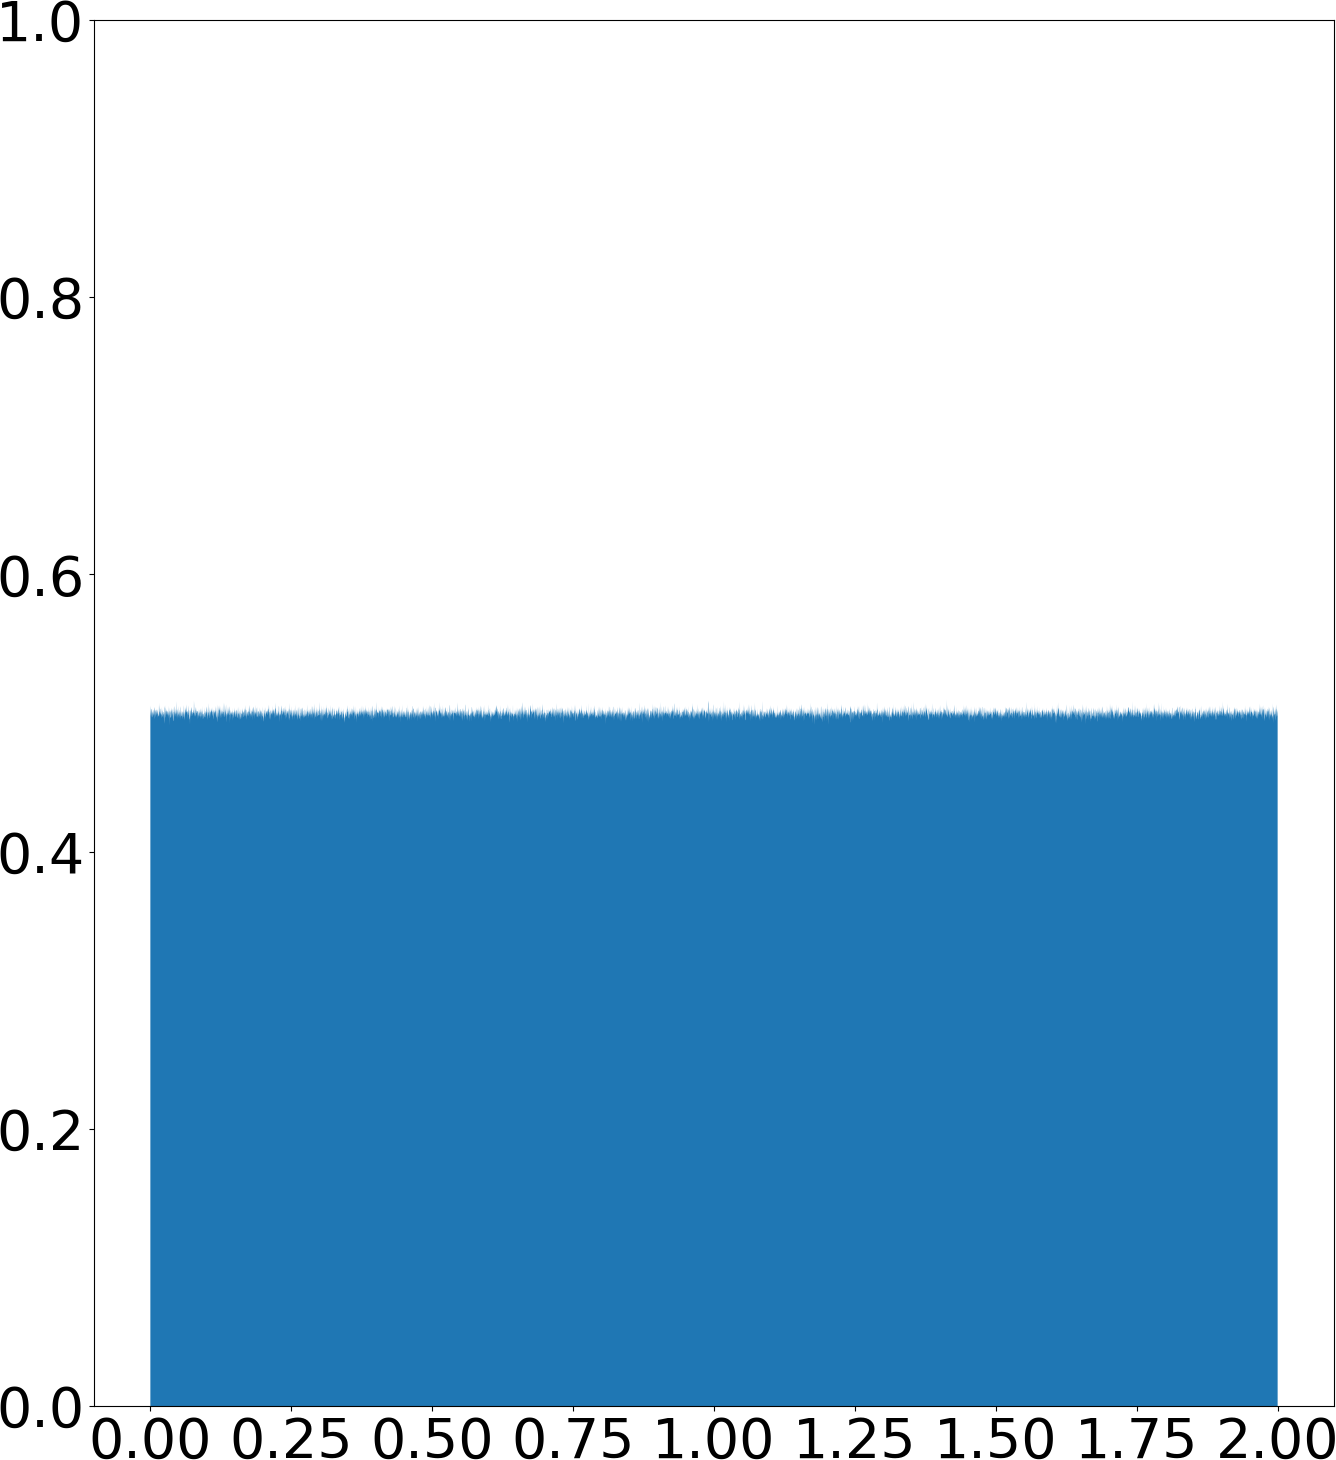
\includegraphics[width=0.48\textwidth]{figure/tent_wave_physical_density_0.2.png}
    \caption{The left column shows the empirical distribution of the shadowing solution for the wave tent map (Eq. \ref{eqn:tent_wave}) at $s=0.05$ (top) and at $s=0.2$ (bottom). The right column shows the probability distribution of a physical solution at the same two values of $s = 0.05$ (top) and $s = 0.2$ (bottom).}
    \label{fig:tent_wave_shadow}
\end{figure}
Hence, we can once again conclude that almost every solution, which is physical, 
has a corresponding shadowing solution, that is non-physical. In this section,
we have shown that the same conclusion holds for several different perturbations 
of the tent map. The physical solutions were distributed nonuniformly 
and differently from one another. However, we observed a commonality in the different perturbations: the shadowing solutions corresponding to almost every physical solution had a fractal-like probability distribution that did not resemble the distributions of the physical solutions in any case. Thus, we have shown significant evidence, through analytical constructions of perturbed tent maps in this section and 
section \ref{sec:quasiphysical} that shadowing solutions can almost surely be nonphysical.

\subsection{What about the Lorenz equation?}
In order to analyze the behavior of the shadowing solutions of the Lorenz'63 system 
of equations, we first make a closed form approximation of the Lorenz map (see section \ref{sec:lorenzMapApprox} of the supplementary material). The reason 
is that except at rare parameter values, the Lorenz system does not have 
solutions that shadow perturbed orbits for all time, but rather only for a finite time 
\cite{lorenzPOTP}. Hence, the Lorenz map also does not have infinitely long shadowing solutions. This implies that a numerical solution of the Lorenz map approximates 
a true solution, as accurately as desired, only for a finite time.

A closed form approximation is constructed by regression performed using long solutions 
of the Lorenz map (see Figure \ref{fig:lorenz_map}). 
\begin{figure}[H]
    \centering
    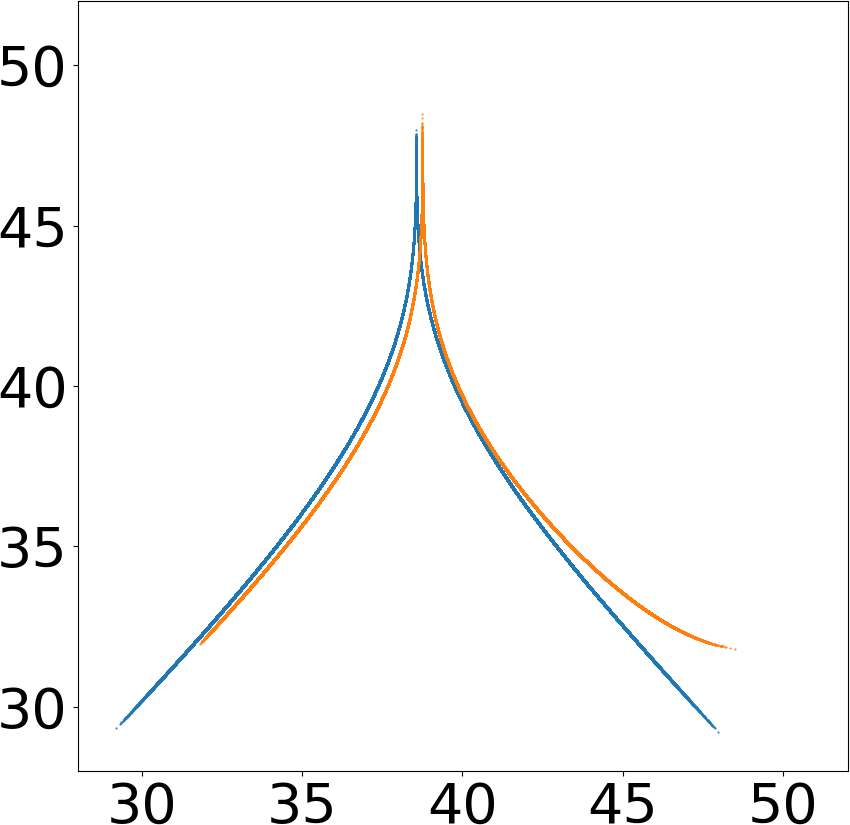
\includegraphics[width=0.32\textwidth]{figure/lorenz_zmax_sigma.png}
    \hspace{0.005\textwidth}
    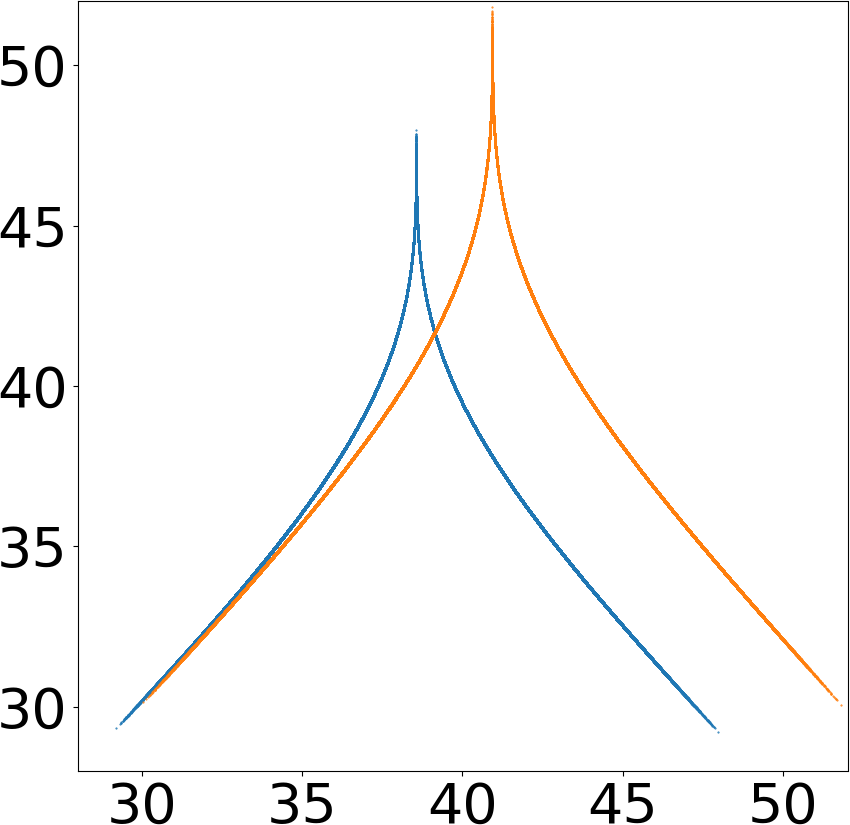
\includegraphics[width=0.32\textwidth]{figure/lorenz_zmax_rho.png}
    \hspace{0.005\textwidth}
    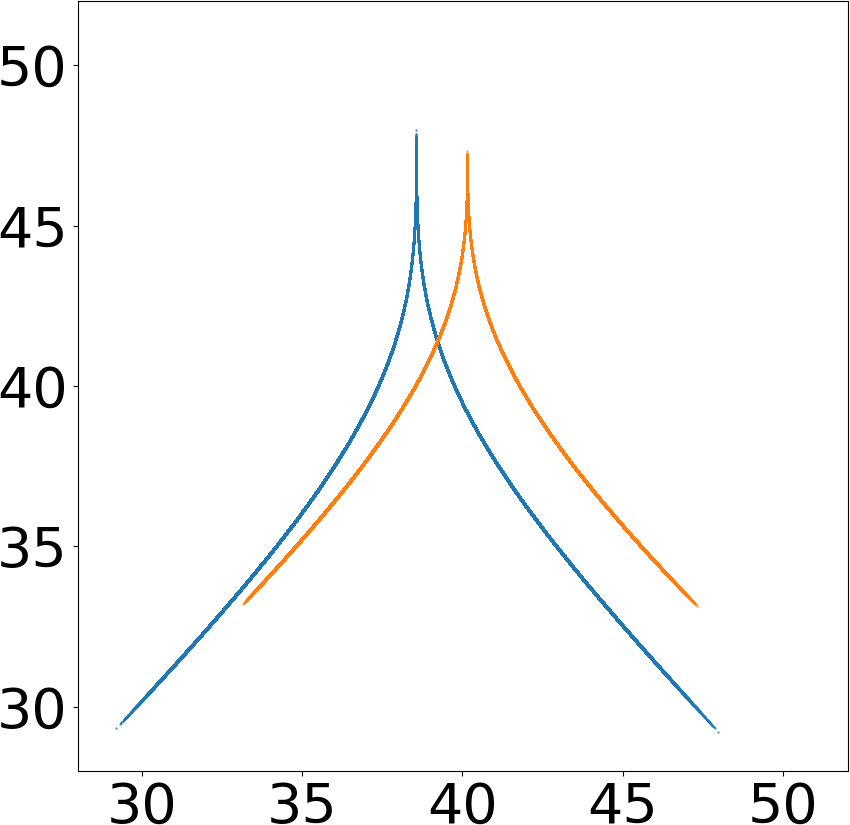
\includegraphics[width=0.32\textwidth]{figure/lorenz_zmax_beta.png}
    \caption{The left, center, and right plots show the effect of the
    parameters $\sigma, \rho$, and $\beta$ on the Lorenz map, respectively.
    In the left plot, the blue, orange, and green lines represent
    $\sigma=10,11$, and $12$, respectively, while $\rho  = 28$ and $\beta = 8/3.$
    In the center plot, the blue, orange, and green lines represent
    $\rho=28,29$ and $30$, respectively, while $\sigma = 10$ and $\beta  = 8/3.$ 
    In the right plot, the blue, orange, and green lines represent
    $\sigma=8/3,3$ and $10/3$ respectively, while $\sigma = 10$ and $\rho = 28.$\nisha{Is the green line overlapping one of the two lines?}}
    \label{fig:lorenz_params}
\end{figure}
The Lorenz map approximation obtained this way is illustrated in Figure \ref{fig:lorenz_params}, for variations of the parameters around their standard values of 
$\rho = 28, \sigma = 10, \beta = 8/3.$ For a range of parameter values, it is numerically verified that the approximate Lorenz map qualitatively reproduces the behavior of the true Lorenz map. Using the approximate Lorenz map, we calculate next the shadowing solutions (see the supplementary material section \ref{sec:lorenzShadowingProcedure} for the numerical procedure). 
\begin{figure}[H]
    \centering
    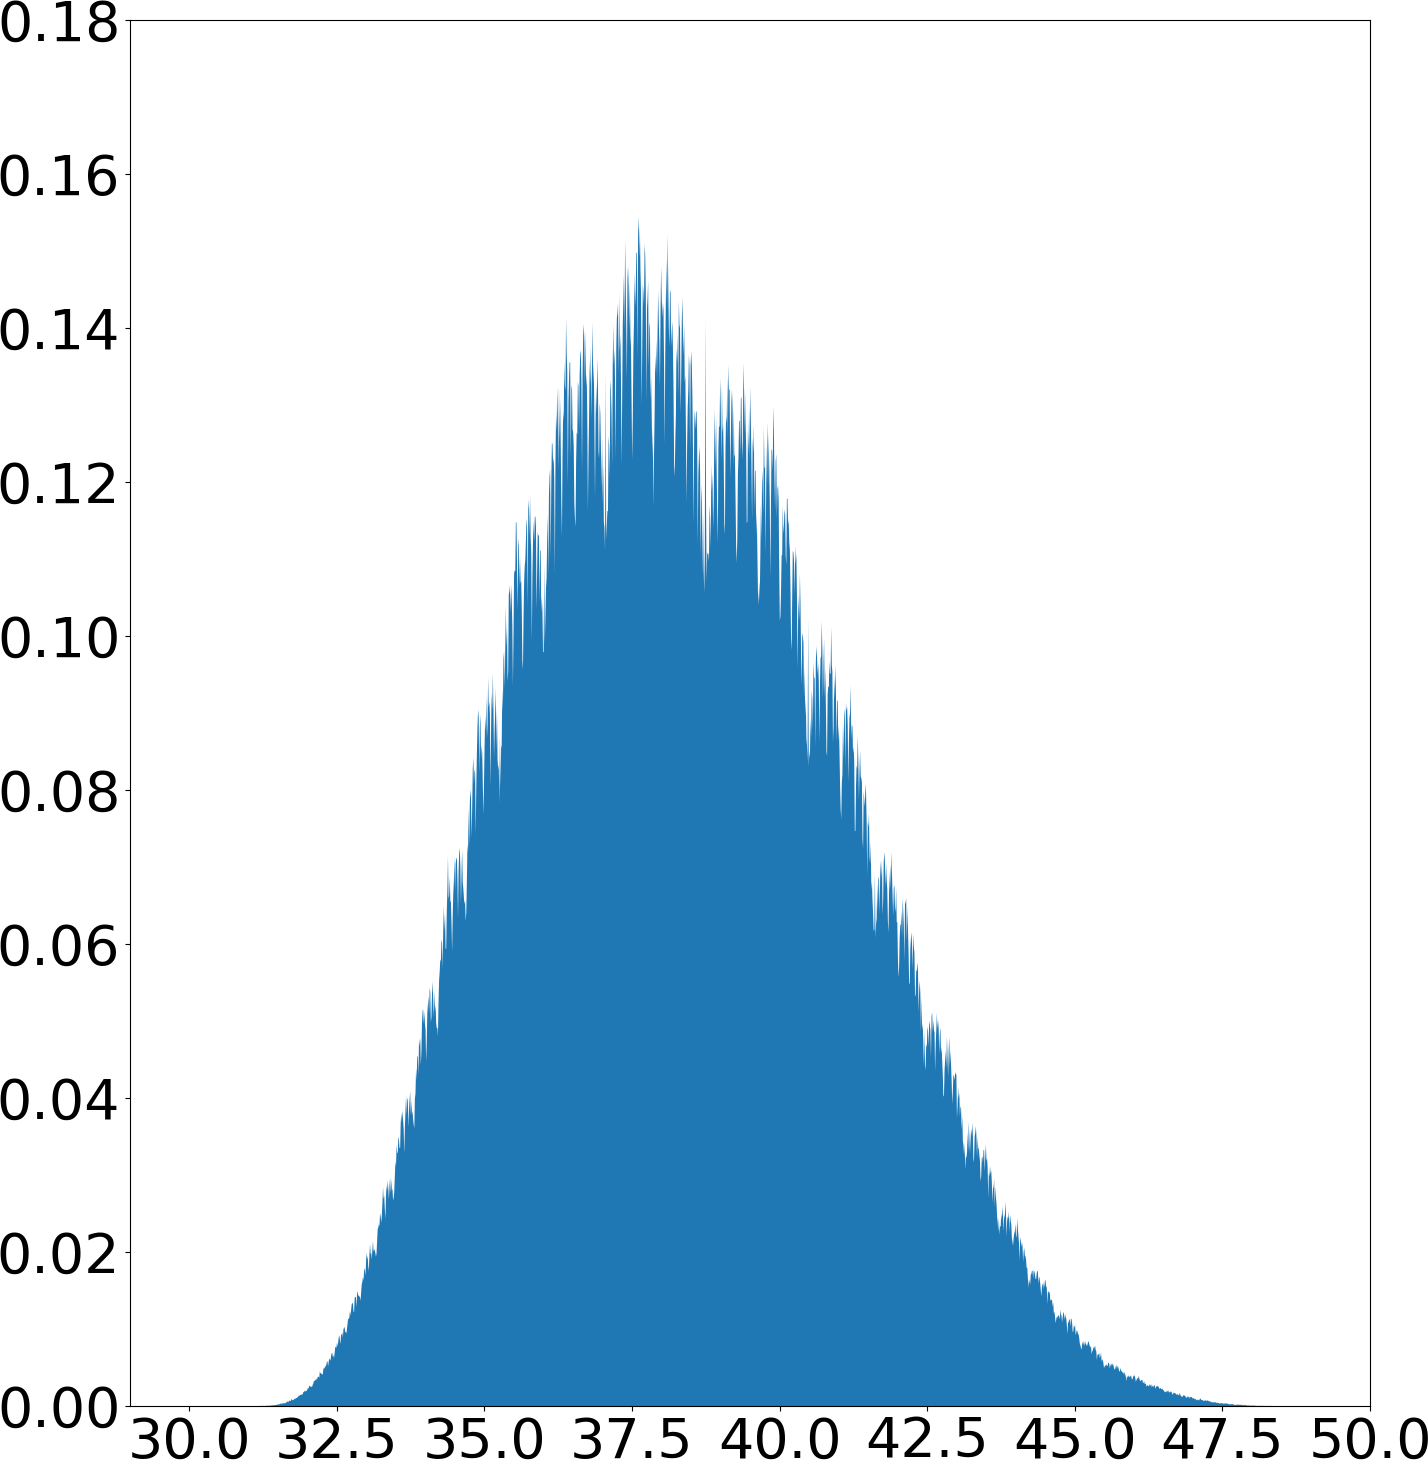
\includegraphics[width=0.48\textwidth]{figure/lorenz_shadow_density_lorenz_zmax_15_28_2.67.json.png}
    \hspace{0.005\textwidth}
    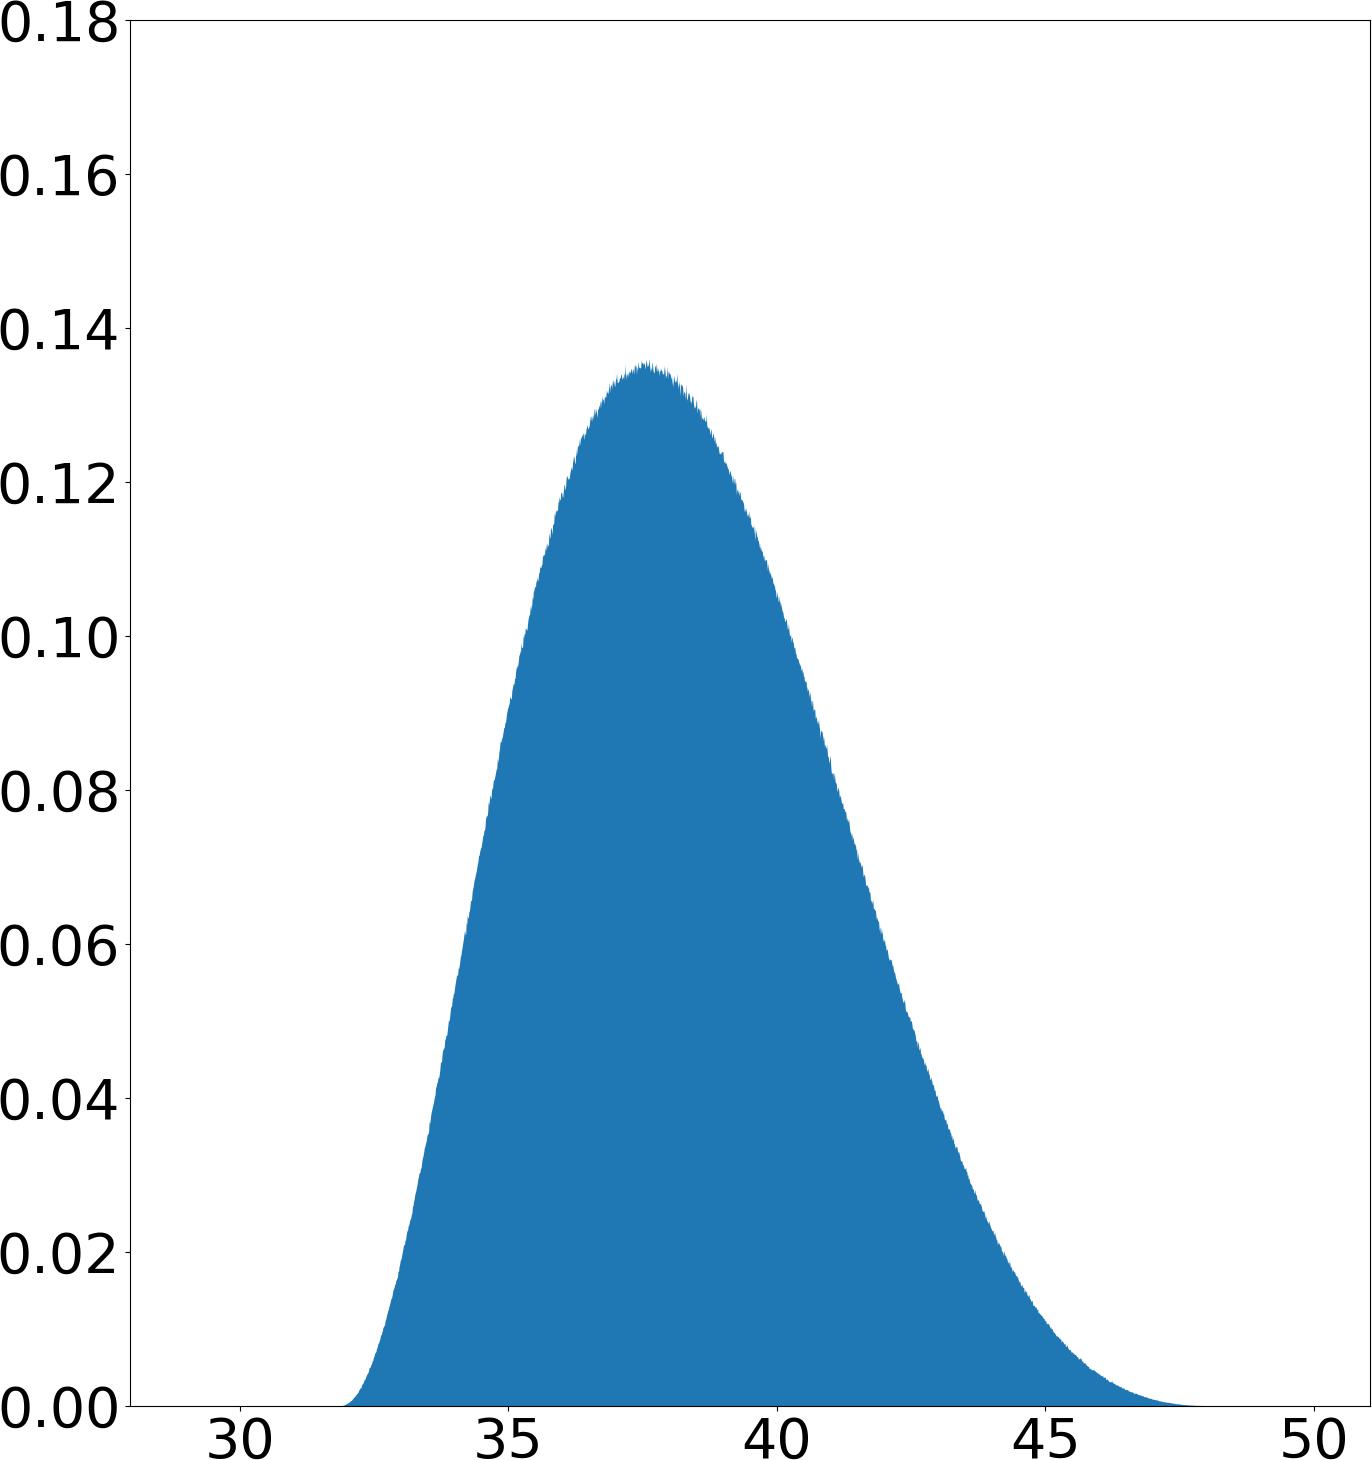
\includegraphics[width=0.48\textwidth]{figure/baseline_density_lorenz_zmax_15_28_2.67.json.png}
    \\
    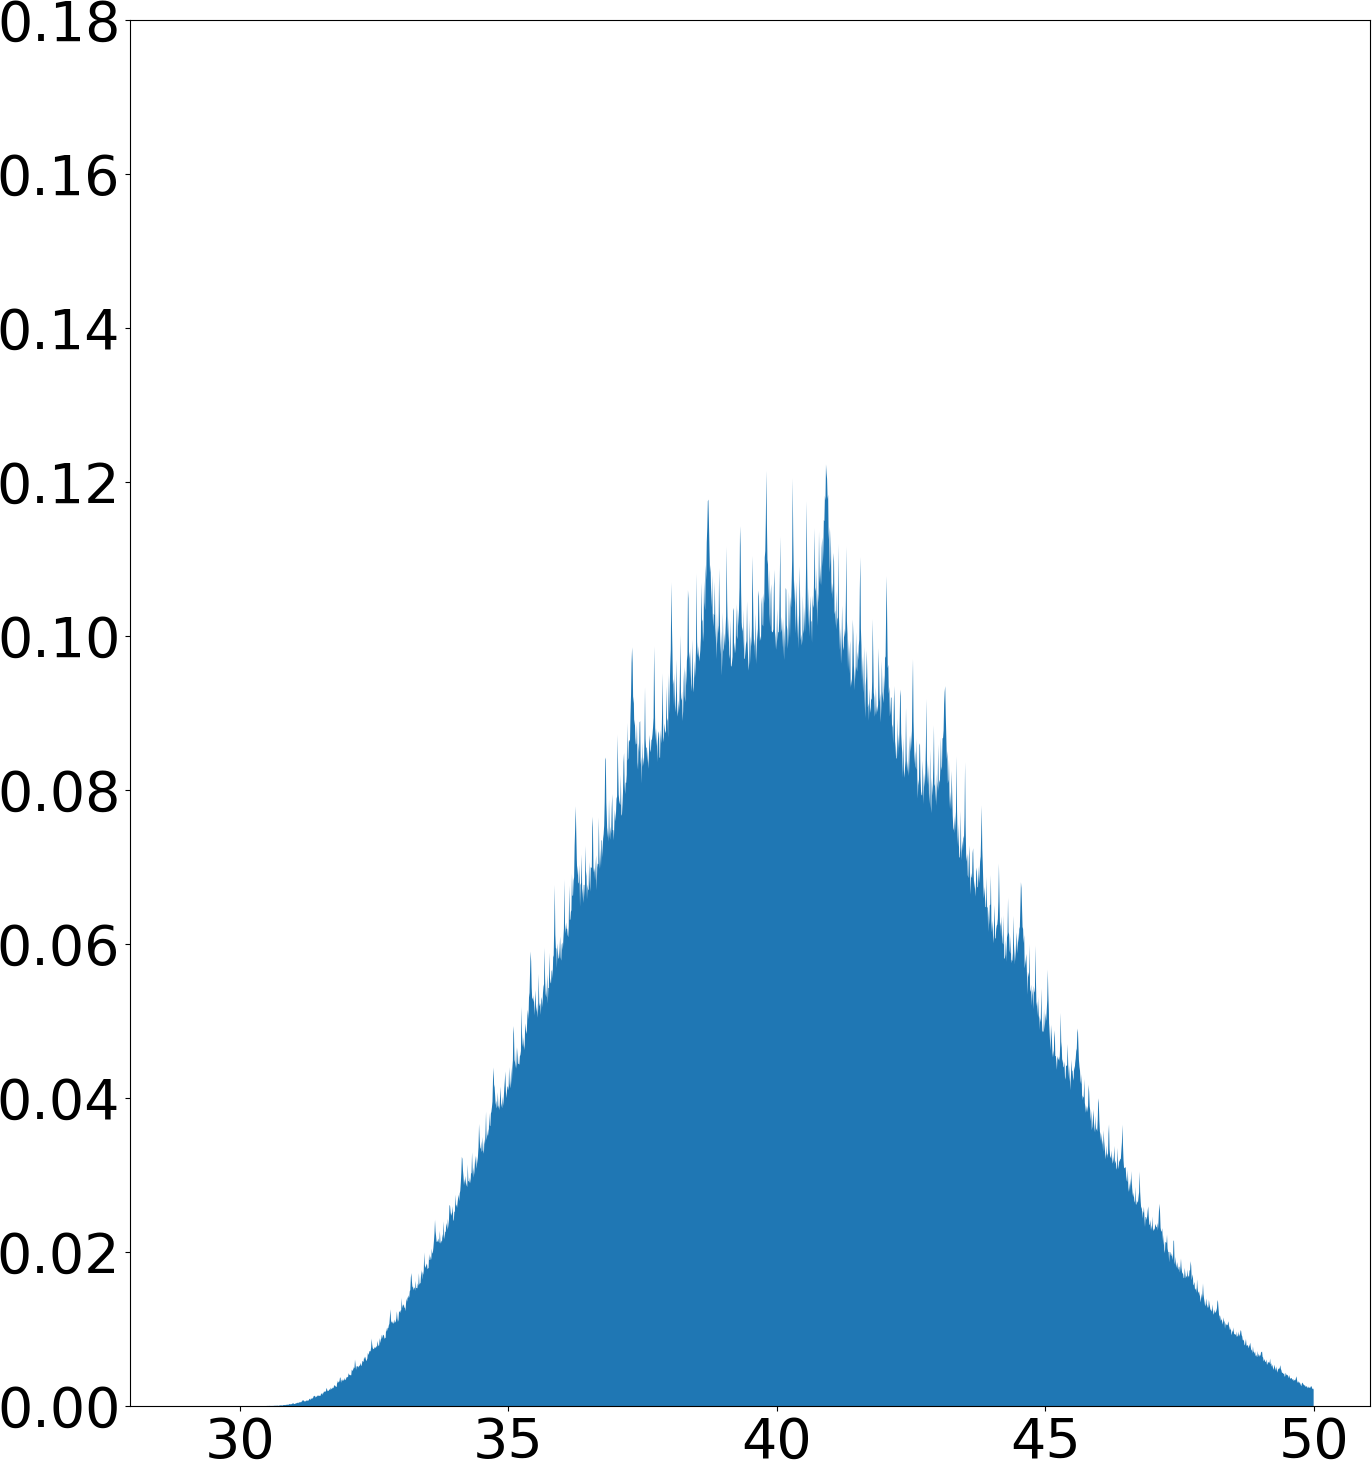
\includegraphics[width=0.48\textwidth]{figure/lorenz_shadow_density_lorenz_zmax_10_30_2.67.json.png}
    \hspace{0.005\textwidth}
    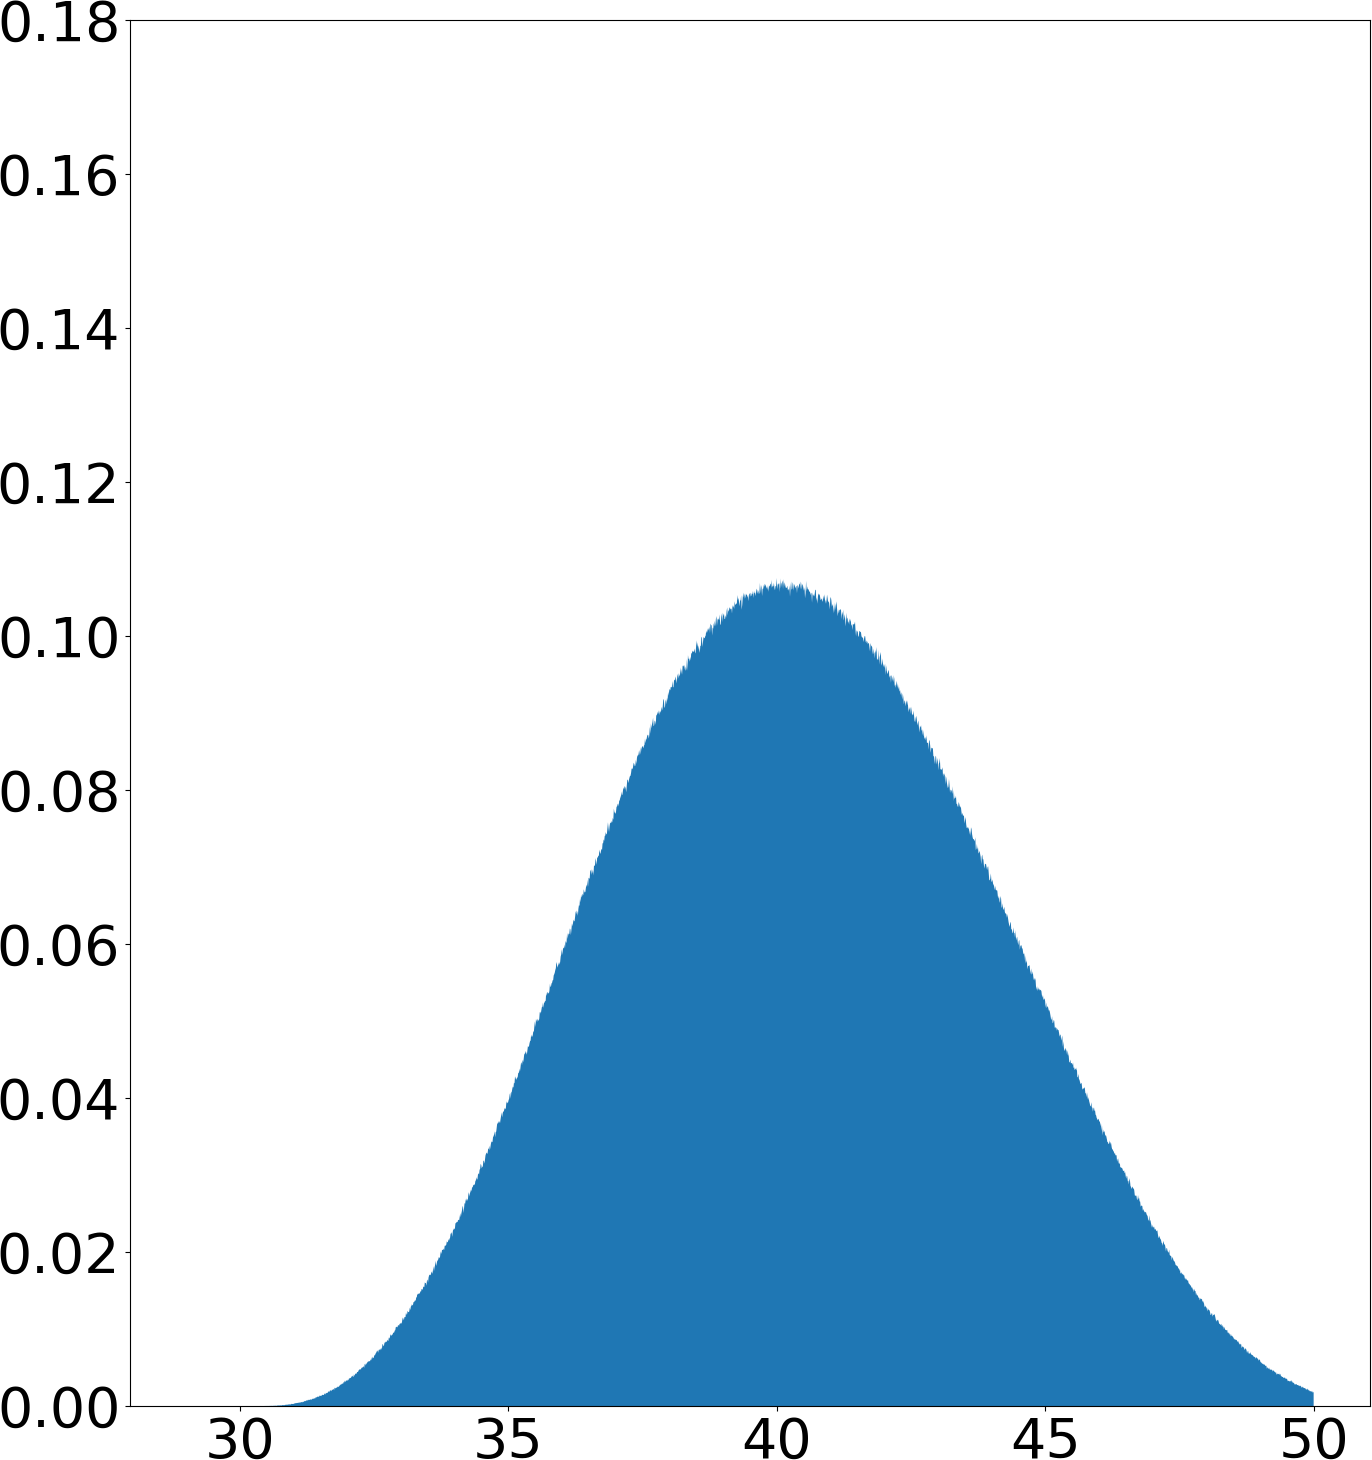
\includegraphics[width=0.48\textwidth]{figure/baseline_density_lorenz_zmax_10_30_2.67.json.png}
    \\
    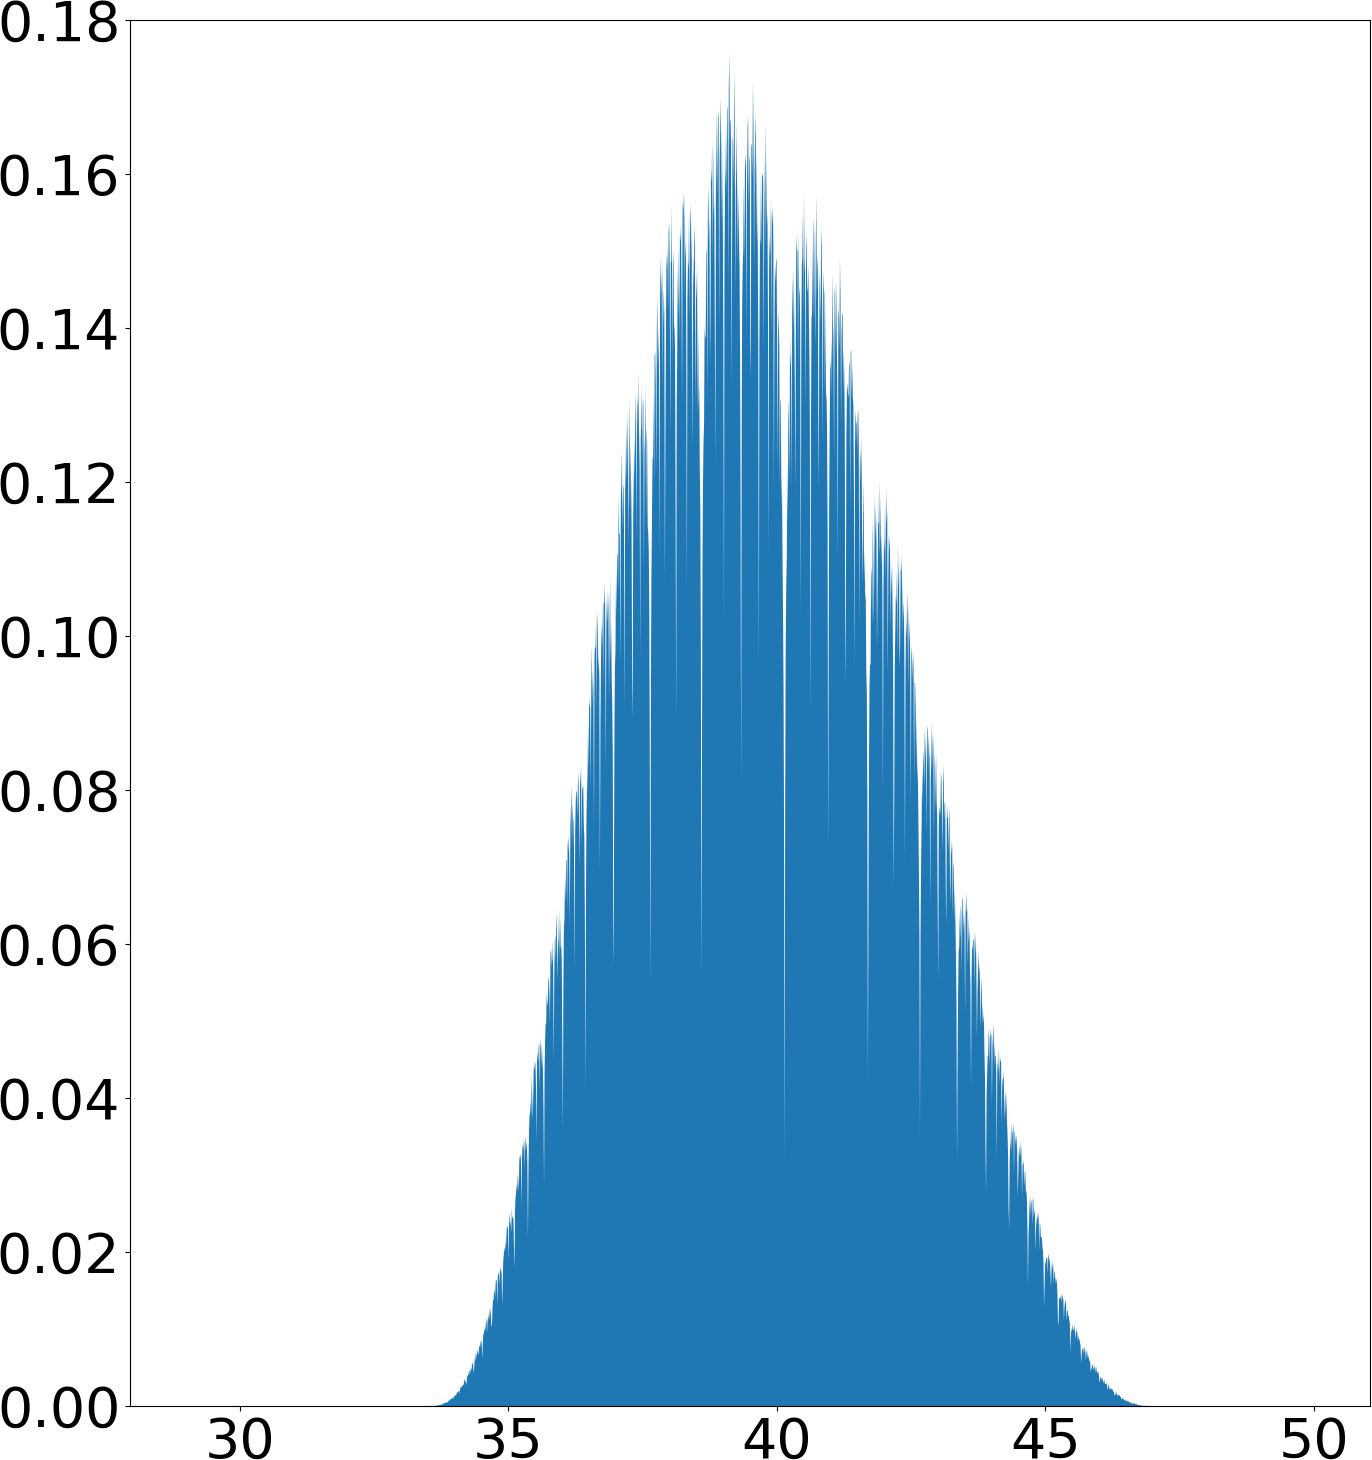
\includegraphics[width=0.48\textwidth]{figure/lorenz_shadow_density_lorenz_zmax_10_28_3.33.json.png}
    \hspace{0.005\textwidth}
    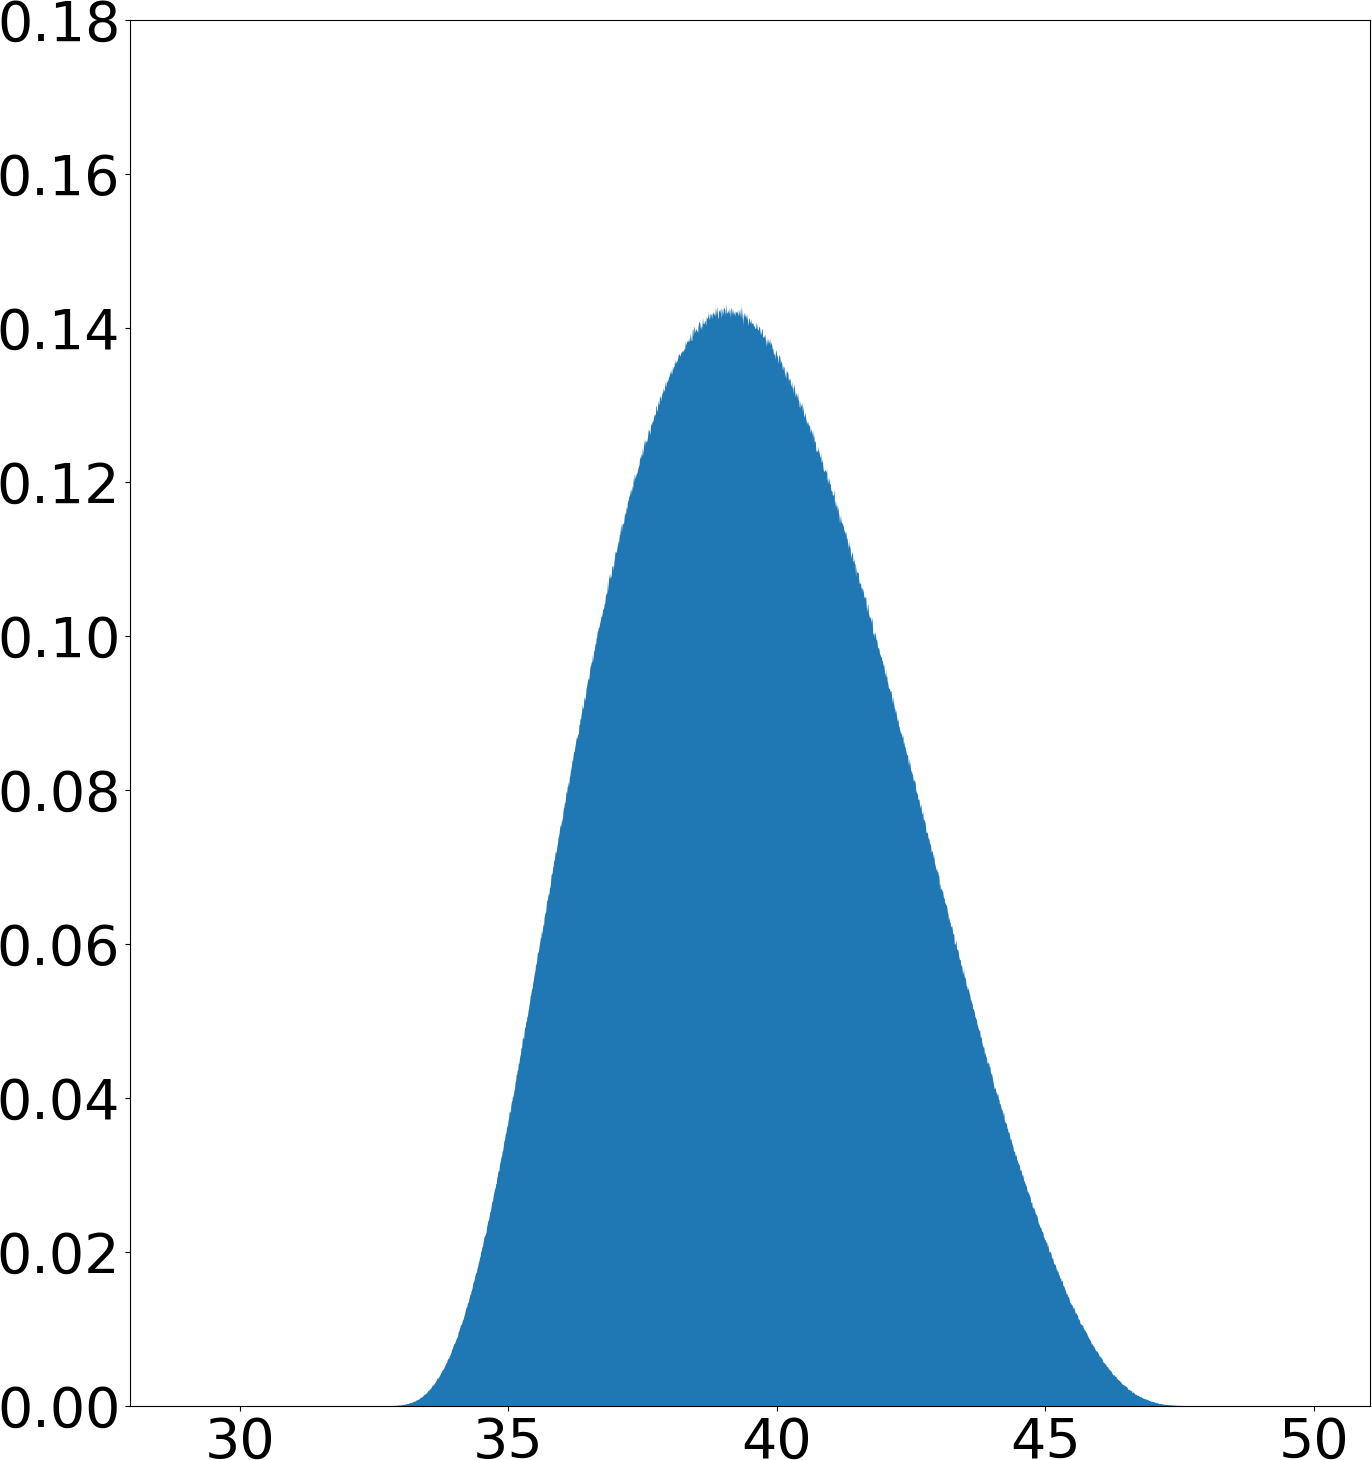
\includegraphics[width=0.48\textwidth]{figure/baseline_density_lorenz_zmax_10_28_3.33.json.png}
    \caption{The left column shows the empirical distribution of the shadowing solution of the Lorenz map at $\rho = 28$ (top row), $\rho = 29$ (middle row), and $\beta = 10/3$ (bottom row). The right column shows the probability distribution of the corresponding physical solution. In each case, the parameters not mentioned are held at their standard values of $\rho = 28, \sigma = 10, \beta = 8/3.$
    }
    \label{fig:lorenz_params_scaled}
\end{figure}
The empirical densities computed from long shadowing solutions, of length 10 billion, are shown in the left column of Figure \ref{fig:lorenz_params_scaled} at three different sets of parameter values, which are also different from the standard values of $\rho = 28, \sigma = 10$, and $\beta = 8/3$. 
In the top and middle row, $\rho = 29$ and $\rho = 30$ are used, respectively, while the other two parameters are retained at their standard values. In the bottom row, only the parameter $\beta$ is perturbed from the standard values; $\beta = 10/3$ is used. On the right column, we plot the densities of physical solutions, the SRB distribution, at the set of parameters corresponding to each row. We again notice that, while the physical distributions are smooth, the shadowing solutions have a rough distribution that appears to have hair-like patterns. Thus, we draw the same conclusion in the Lorenz map as in the various perturbations of the tent map treated in section \ref{sec:tent}: shadowing solutions do not have the same distribution as a typically observed solution of the governing equation. In other words, shadowing solutions may be nonphysical.


\section{Discussions}
Through a rigorous counter-example, we show that shadowing can lead
to nonphysical solutions.  The conclusion has an immediate implication for
sensitivity analysis methods based on the concept of shadowing \cite{qiqi-lss}\cite{angxiu-lss}\cite{lasagne}.
When the goal is to compute derivatives of ensemble averages, where the ensemble
is distributed according to the physical measure, i.e., the SRB measure, shadowing-based methods can give wrong results.  This has been observed
before and appropriately attributed as ``ergodicity breaking error'' \cite{patrick} \cite{angxiu-error}. In this paper, we construct rigorous analytical examples of this error.

Even more troubling is the implication for numerical simulations of chaotic
governing equations.  Through the examples in this paper, it is clear that a numerical solution, satisfying
a governing equation perturbed due to numerics, is not expected to shadow a
physical solution of the real governing physics.  What is, if any, the
relation of a numerical solution, such as DNS of turbulent flows, to
the true physics? While this question remains open, we conclude with a final example illustrating that not only can shadowing solutions display statistical averages different from physical solutions, but that the difference can be drastic. 
For $10^{-18}$ perturbation (trunction numerically), we get completely different statistics. How can we trust numerical solutions

[Nisha: Eq. 18 and Eq. 19 - shadowing sensitivities are incorrect.]

\begin{figure}
    \centering
    \includegraphics[width=0.35\textwidth,height=2in]{figure/mapn0s0.png}
    \includegraphics[width=0.35\textwidth,height=2in]{figure/mapn5s0.1.png}
    \caption{Two chaotic maps (in red) and their associated stationary  distributions (in purple). The map on the right is only an \emph{infinitesimal} perturbation of that on the left; for more information see \cite{desmos}.}
    \label{fig:map}
\end{figure}
[Nisha: shadowing perturabtions predict tiny effects. Real effect is a lot more dramatic. Desmos plot.]
% give example of numerics that destroys physicalness

\bibliographystyle{spmpsci}
\bibliography{refs.bib}
\section{Supplementary material}
\subsection{The Lorenz Map}
\subsection{Approximation of the Lorenz Map}

\subsubsection{Computing shadowing solution of the Lorenz map}
In this section, we discuss how to numerically compute the shadowing trajectories of the Lorenz map. One of the motivations for approximating the Lorenz map is that having a closed form expression is necessary in the algorithm we discuss for numerical shadowing solution computation. The program used to generate Figure 
\ref{fig:lorenz_params_scaled} is in \verb+lorenz_map/shadow.py+. The main logic behind the numerical procedure to compute the shadowing solution can be found in that script, within the function \verb+shadow+, which calls \verb+find2+. Let $x_n, n = 0,1,2,3\cdots,N$ be a given perturbed solution given to us until time $N$. The goal is to find a sequence $\left\{ y_n\right\}_{n=0}^{N}$ that is a shadowing solution. This means that $y_n$ must satisfy the governing equation: $y_{n+1} = \varphi(y_n),$ where $\varphi$ is the Lorenz map, and, 
$y_n$ and $x_n$ must stay close to each to other for the length of time, $N$. We find the sequence $y_n$ backward in time. Let $z_{\rm sep,s}$ be the $z$-location of the cusp of the perturbed Lorenz map that generated $x_n$; to indicate the original map, we omit the $s$ in the subscript. We split the domain into two regions, $[z_{\rm min}, z_{\rm sep}]$ and $(z_{\rm sep}, z_{\rm max}],$ and 
obtain, for $n = N-1, \cdots, 0,$
\begin{align}
    y_n = \begin{cases}
                     z_{\rm sep} + f(y_{n+1}), & x_n > z_{\rm sep, s} \\
                     z_{\rm sep} - f(y_{n+1}), & x_n \leq z_{\rm sep, s}.
    \end{cases}
    \label{eqn:shadowingFormula}
\end{align}
Here the function $f$ is implemented in 
\verb+find2+. Inside \verb+find2+, given a $y$, 
a recursive procedure is used to 
find a number $v_k = f(y_{n+1})$ such that if $y_n$ set 
using Eq. \ref{eqn:shadowingFormula} is (approximately) the shadowing 
solution. At $n = N-1,$ $y_N$ is initialized with a random guess close to $x_N.$
Then, the following recursive equation is solved to compute $f(y_{n+1})$.
\begin{align}
        v_{k+1} = v_k \;  \exp{\big({y_{n+1} - \varphi(y_{n,k})}\big)} \; \exp{\Big(\dfrac{-1}{\varphi'(y_{n,k}) v_k}\Big)}, \; k = 0,1,\cdots,
\end{align}
At $k=0,$ we randomly assign $v_0 = 1,$ and continue the above iteration 
until $|v_k|$, and $|y_{n+1} - \varphi(y_{n,k})|$ are both less than 
a tolerance. When the iteration converges, at some $k$,
$f_i(y_{n+1}) = v_k.$ Notice that by construction, the
sequence $\left\{ y_n\right\}$ computed this way is a shadowing solution.
\end{document}
